\documentclass[a5paper]{ufsc-thesis}
\usepackage[utf8]{inputenc}

\title{Aplicação do modelo de atores em um programa de teste e diagnóstico de circuitos eletrônicos}
\author{Antonio Carlos Luppi Junior}
\date{Julho 2017}
\local{Florianópolis}
\orientador{Prof. Fernando Rangel de Sousa}
%\coorientador{Equipe \abnTeX}
\instituicao{%
  Universidade Federal de Santa Catarina -- UFSC
  \par
  Departamento de Engenharia Elétrica e Eletrônica
  \par
  Programa de Graduação}
\tipotrabalho{Trabalho de Conclusão de Curso}
% O preambulo deve conter o tipo do trabalho, o objetivo, 
% o nome da instituição e a área de concentração 
\preambulo{Monografia submetida ao Departamento de Engenharia Elétrica e Eletrônica da Universidade Federal de Santa Catarina como requisito da disciplina EEL7890 - Trabalho de Conclusão de Curso.}

\usepackage{relsize}
\usepackage{booktabs}
%\usepackage{multirow} % para gerar tabelas
\usepackage[table,xcdraw]{xcolor} % para gerar tabelas
% \documentclass[xcolor=table]{beamer}
\usepackage[authoryear,sort,elide]{natbib}
\usepackage{array}
\usepackage{pdfpages}

%suporte à portugues brasileiro
\usepackage[brazil]{babel}	% for multilingual support
\usepackage[utf8]{inputenc} % for use utf8
\usepackage[T1]{fontenc}
%https://pt.sharelatex.com/learn/Portuguese

%suporte matematico e gráfico
\usepackage{amstext,amsmath}
\usepackage{graphicx}
\usepackage{calc}
\graphicspath{ {fig/} }
\usepackage{subcaption} % Para usar duas ou mais figuras como uma só. [caption=false]
\usepackage[a5paper]{geometry}
%\usepackage[alf]{abntex2cite}
\usepackage{textcomp} % para usar o simbolo de trademark

\usepackage{tabularx}  % for 'tabularx' environment and 'X' column type
\usepackage{ragged2e}  % for '\RaggedRight' macro (allows hyphenation)
\newcolumntype{Y}{>{\RaggedRight\arraybackslash}X} 

\newcommand{\specialcell}[2][c]{%
  \begin{tabular}[#1]{@{}c@{}}#2\end{tabular}}

\begin{document}
%\frontmatter
\pretextual
\imprimircapa
\imprimirfolhaderosto*

\begin{fichacatalografica}
    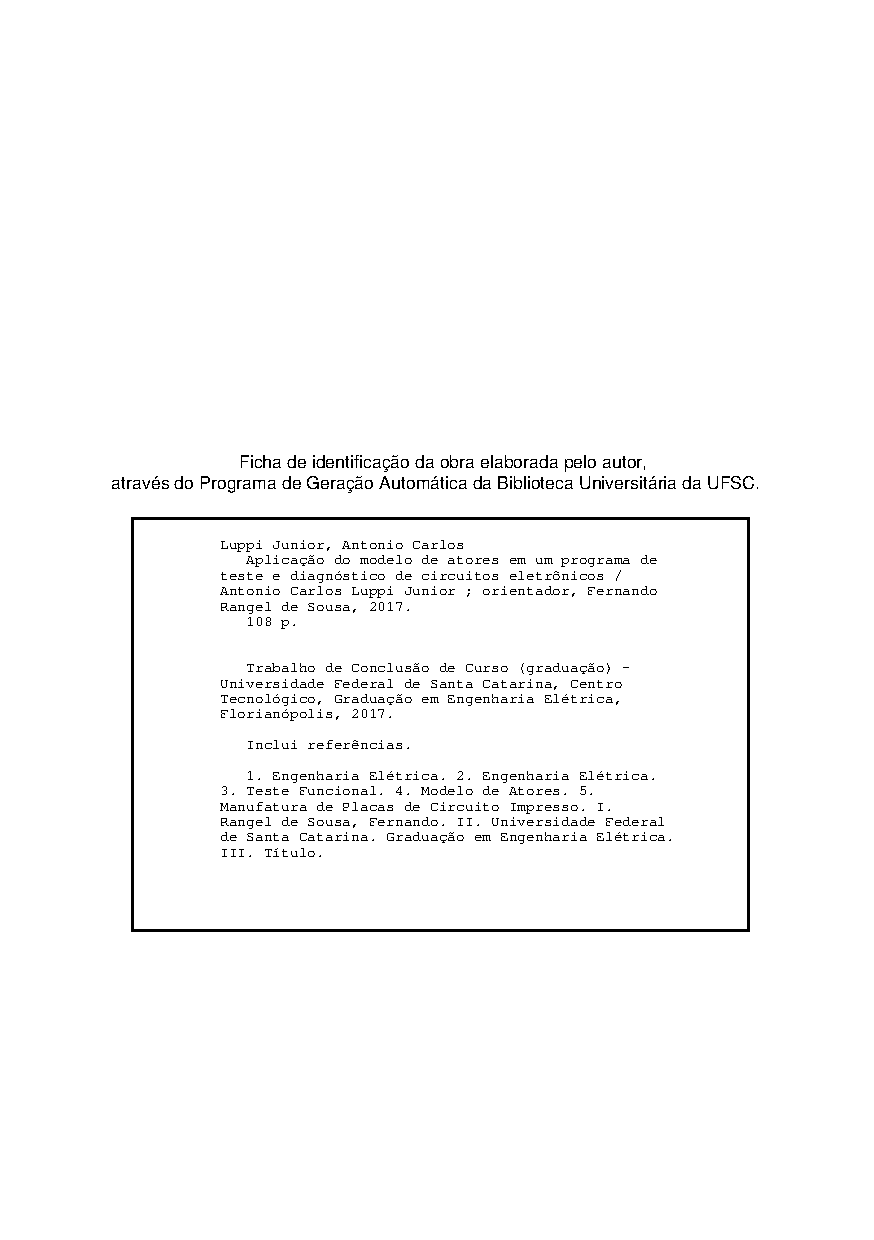
\includepdf{Ficha_Catalografica.pdf}
\end{fichacatalografica}

\begin{folhadeaprovacao}
    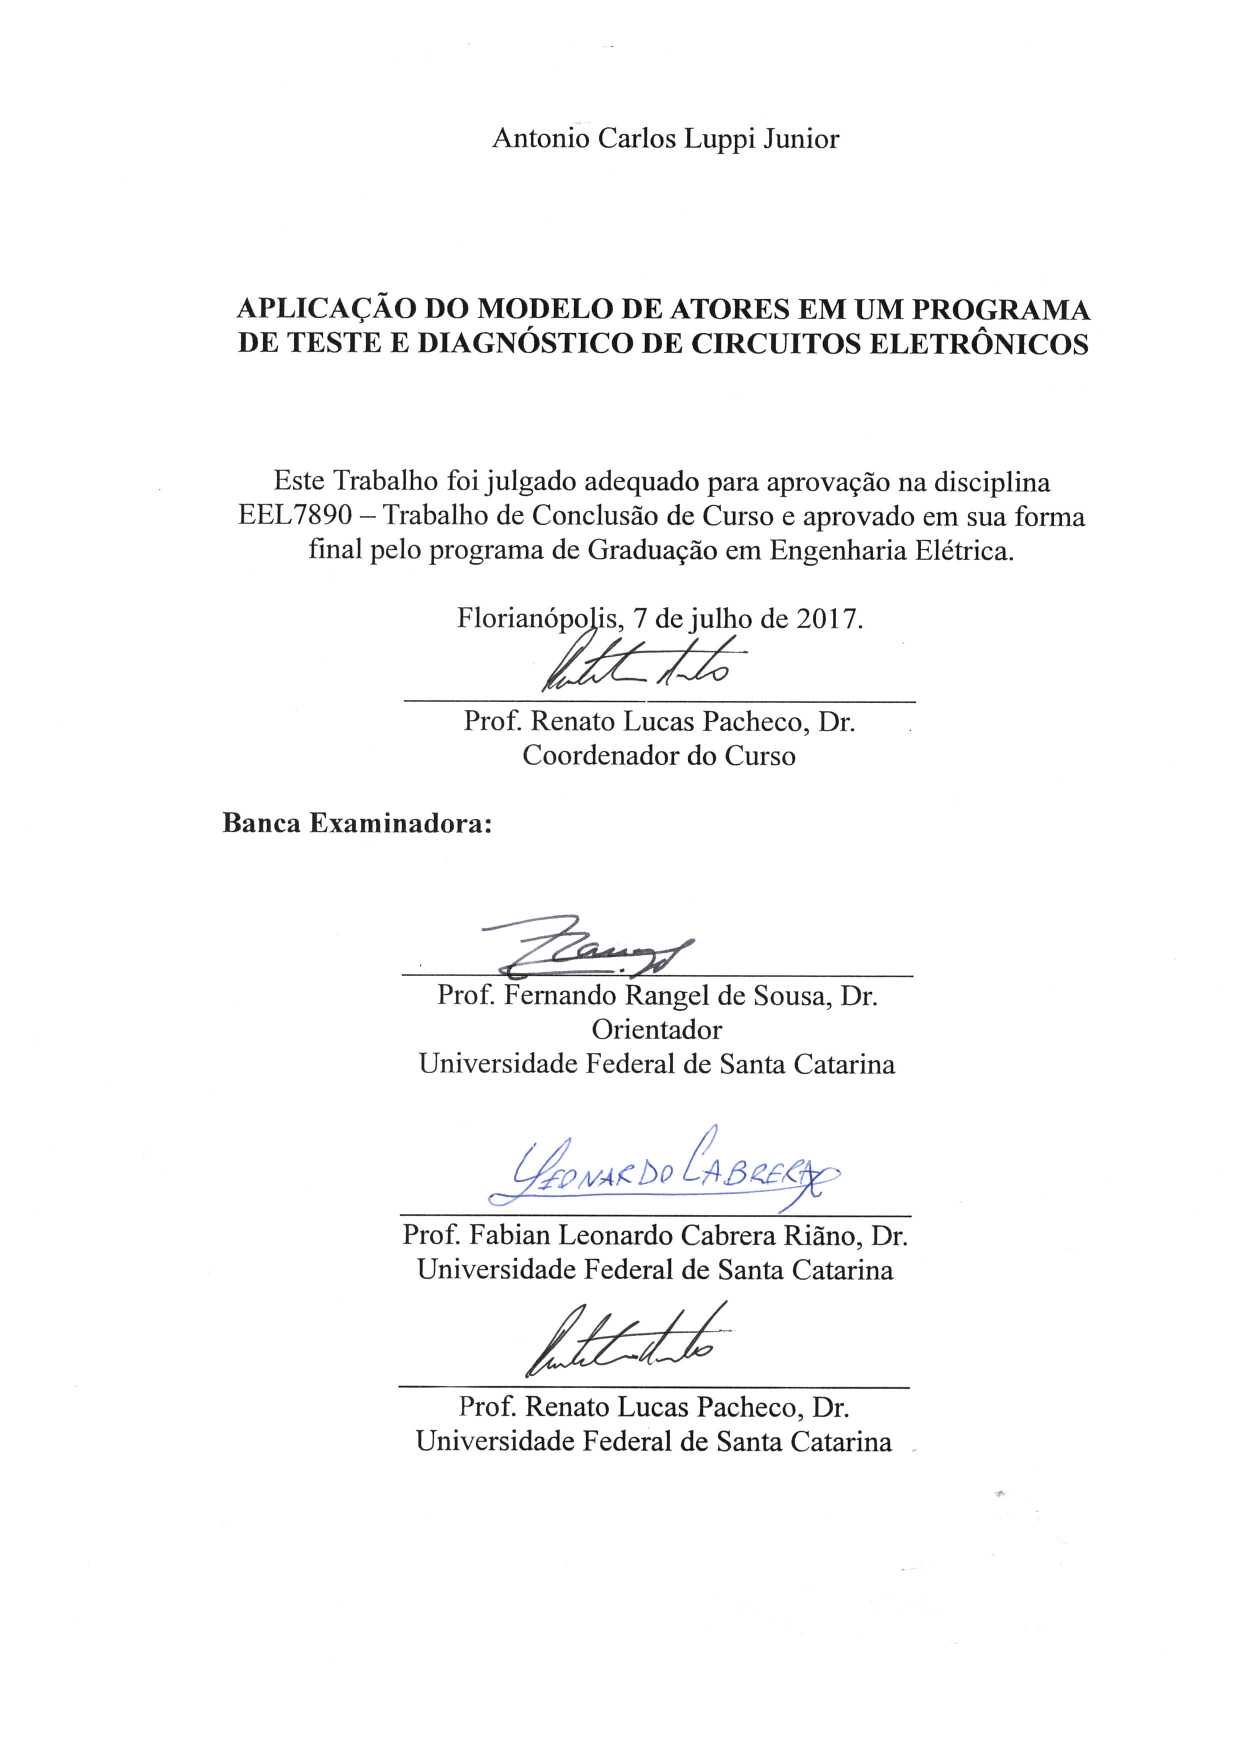
\includepdf{folhaaprovacao.pdf}
\end{folhadeaprovacao}

    % ---
% Inserir a ficha bibliografica
% ---

% Isto é um exemplo de Ficha Catalográfica, ou ``Dados internacionais de
% catalogação-na-publicação''. Você pode utilizar este modelo como referência. 
% Porém, provavelmente a biblioteca da sua universidade lhe fornecerá um PDF
% com a ficha catalográfica definitiva após a defesa do trabalho. Quando estiver
% com o documento, salve-o como PDF no diretório do seu projeto e substitua todo
% o conteúdo de implementação deste arquivo pelo comando abaixo:
%

%\imprimirfichacatalografica
\begin{comment}
\begin{fichacatalografica}
	\vspace*{\fill}					% Posição vertical
	\hrule							% Linha horizontal
	\begin{center}					% Minipage Centralizado
	\begin{minipage}[c]{12.5cm}		% Largura
	
	\imprimirautor
	
	\hspace{0.5cm} \imprimirtitulo  / \imprimirautor. --
	\imprimirlocal, \imprimirdata-
	
	\hspace{0.5cm} \pageref{LastPage} p. : il. (algumas color.) ; 30 cm.\\
	
	\hspace{0.5cm} \imprimirorientadorRotulo~\imprimirorientador\\
	
	\hspace{0.5cm}
	\parbox[t]{\textwidth}{\imprimirtipotrabalho~--~\imprimirinstituicao,
	\imprimirdata.}\\
	
	\hspace{0.5cm}
		1. Palavra-chave1.
		2. Palavra-chave2.
		I. Orientador.
		II. Universidade Federal de Santa Catarina.
		III. Departamento de Engenharia Elétrica e Eletrônica.
		IV. Título\\ 			
	
	\hspace{8.75cm} CDU 02:141:005.7\\
	
	\end{minipage}
	\end{center}
	\hrule
\end{fichacatalografica}
\end{comment}
% ---

% ---
% Inserir errata
%

% ---

% ---
% Inserir folha de aprovação
% ---

% Isto é um exemplo de Folha de aprovação, elemento obrigatório da NBR
% 14724/2011 (seção 4.2.1.3). Você pode utilizar este modelo até a aprovação
% do trabalho. Após isso, substitua todo o conteúdo deste arquivo por uma
% imagem da página assinada pela banca com o comando abaixo:
%
%

\begin{comment}
\begin{folhadeaprovacao}

  \begin{center}
    {\ABNTEXchapterfont\large\imprimirautor}

    \vspace*{\fill}\vspace*{\fill}
    \begin{center}
      \ABNTEXchapterfont\bfseries\Large\imprimirtitulo
    \end{center}
    \vspace*{\fill}
    
    \hspace{.45\textwidth}
    \begin{minipage}{.5\textwidth}
        \imprimirpreambulo
    \end{minipage}%
    \vspace*{\fill}
   \end{center}
        
   Trabalho aprovado. \imprimirlocal, 07 de Julho de 2017:

   \assinatura{\textbf{\imprimirorientador, Dr.} \\ Orientador \\ Universidade Federal de Santa Catarina} 
   \assinatura{\textbf{Fabian Leonardo Cabrera Riano, Dr.}  \\ Universidade Federal de Santa Catarina}
   \assinatura{\textbf{Renato Lucas Pacheco, Dr.}  \\ Universidade Federal de Santa Catarina}
   %\assinatura{\textbf{Professor} \\ Convidado 3}
   %\assinatura{\textbf{Professor} \\ Convidado 4}
      
   \begin{center}
    \vspace*{0.5cm}
    {\large\imprimirlocal}
    \par
    {\large\imprimirdata}
    \vspace*{1cm}
  \end{center}
  
\end{folhadeaprovacao}
\end{comment}
% ---

% ---
% Dedicatória
% ---
\begin{dedicatoria}
   \vspace*{\fill}
   \centering
   \noindent
    \textit{Este trabalho é dedicado à minha mãe.} \vspace*{\fill}
\end{dedicatoria}
% ---

% ---
% Agradecimentos
% ---
\begin{agradecimentos}



Agradeço primeiramente ao Professor Fernando Rangel pela paciência e profissionalismo em me orientar neste trabalho. Agradeço à Universidade Federal de Santa Catarina por me proporcionar educação gratuita e de qualidade, não só profissional como também cidadã.

Agradeço à Heloisa pelas muitas revisões textuais e pelo suporte e carinho em todos os momentos. 
Aos meus amigos de graduação pelo companheirismo neste anos de UFSC, em especial ao Lucas Stéfano, por revisar meu trabalho. E por fim, agradeço à Mirian, minha mãe, pelo apoio incondicional.

\end{agradecimentos}
% ---



% ---
% RESUMOS
% ---

% resumo em português
\setlength{\absparsep}{18pt} % ajusta o espaçamento dos parágrafos do resumo
\begin{resumo}
    Este trabalho relata o processo de desenvolvimento de um software de testes funcionais para validação e detecção de falhas em placas eletrônicas em seu processo produtivo assim como nos retornos de manutenção. Os requisitos de flexibilidade e modularidade levaram a escolha do \textit{framework} de atores, a implementação do Modelo de Atores de computação concorrente em LabVIEW. Foram criadas classes de atores para cada área de competência de teste: interface com multímetros, comunicação com o dispositivo sob teste, teste de potência RF, gerador de registros de teste e o controle de execução. Melhorias em ergonomia foram consideradas durante o processo de desenvolvimento, e testes prévios de execução das rotinas de teste apontaram melhorias no tempo de execução de testes e automatização do processo.
    
 
    \textbf{Palavras-chaves}: teste funcional. teste estrutural. modelo de atores. programação concorrente. LabVIEW. montagem de placas de circuito impresso. 
\end{resumo}

% resumo em inglês
\begin{resumo}[Abstract]
 \begin{otherlanguage*}{english}
   
   This work reports the development process of a functional test sofware for fail detection and validation of assembled circuit boards on their productive process and in field returns. The requirements in flexibility and modularity led to the choice of the actor framework, the Labview implementation of the Actor Model of concurrent computing. Actor classes were developed for each field of competence: multimeter interface, device under test communication, RF power test, test log generator, and execution control. Enhancements in ergonomics were considered during the development process, and prior tests runs of the routines indicated improvements in the test execution time and process automation.
   
   \vspace{\onelineskip}
 
   \noindent 
   \textbf{Key-words}: funcional test. structural test. actor model. concurrent programming. LabVIEW. printed circuit board assembly.
 \end{otherlanguage*}
\end{resumo}

% ---
% inserir lista de ilustrações
% ---
\pdfbookmark[0]{\listfigurename}{lof}
\listoffigures*
\cleardoublepage
% ---

% ---
% inserir lista de tabelas
% ---
\pdfbookmark[0]{\listtablename}{lot}
\listoftables*
\cleardoublepage
% ---

% ---
% inserir lista de abreviaturas e siglas
% ---
\begin{siglas}
    \item [AOI] \textit{Automated Optical Inspection}
    \item [ASIC] \textit{Application-Specific Integrated Circuit}
    \item [ATS] \textit{Automated Test Systems}
    \item [AXI] \textit{Automated X-ray Inspection}
    \item [BERT] \textit{Bit-error Rate}
    \item [BISD] \textit{Build-in Self Diagnosis}
    \item [BIST] \textit{Build-in Self Test}
    \item [BST] \textit{Boundary Scan Test}
    \item [CA] Corrente Alternada
    \item [CAN] \textit{Controller Area Network}
    \item [CC] Corrente Contínua
    \item [DfD] \textit{Design for Debug}
    \item [DfT] \textit{Design for Testability}
    \item [DfY] \textit{Design for Yield}
    \item [EDGE] \textit{Enhanced Data rates for GSM Evolution}
    \item [E/S] Entrada/Saída
    \item [FPGA] \textit{Field-programmable Gate Array}
    \item [FPT] \textit{Flying Probe Test}
    \item [GPRS] \textit{General Packet Radio Service}
    \item [ICL] \textit{Instrument Connectivity Language} 
    \item [ICT] Teste Intra-circuito ou \textit{In-Circuit Test}
    \item [IEEE] \textit{Institute of Electrical and Electronics Engineers}
    \item [IMEI] \textit{International Mobile Equipment Identity}
    \item [IP] \textit{intellectual property}
    \item [JSON] \textit{JavaScript Object Notation}
    \item [JTAG] \textit{Joint Test Action Group}
    \item [LAN] \textit{Local Area Network}
    \item [LIN] \textit{Local Interconnect Network}
    \item [LVDS] \textit{Low Voltage Differential signaling}
    \item [M2M] \textit{Machine-to-machine}
    \item [MDA] \textit{Manufacturing Defect Analysis}
    \item [NFF] \textit{No failure found}
    \item [NoC] \textit{Network-on-a-Chip}
    \item [OEM] \textit{Original Equipment Manufacturer}
    \item [OTAP] \textit{Over-the-air Provisioning}
    \item [PCI] Placa de circuito Impresso
    \item [PCIe] \textit{Peripheral Component Interconnect Express}
    \item [PCB] \textit{Printed Circuit Board}
    \item [PCIM] Placa de circuito impresso e montada
    \item [PDL] \textit{procedural description language}
    \item [PRPG] \textit{Pseudo-random Pattern Generator}
    \item [QA] \textit{Quality Assurance}
    \item [RSN] \textit{Reconfigurable Scaning Networks}
    \item [SATA] \textit{Serial AT Attachment}
    \item [SIM] \textit{Subscriber Identification Module}
    \item [SIMcard] \textit{Subscriber Identification Module card}
    \item [SNR] \textit{Signal-Noise Ratio}
    \item [SPI] \textit{Serial Peripheral Interface}
    \item [SoC] \textit{System-on-a-chip}
    \item [SubVI] \textit{Sub Virtual Instrument}
    \item [UART] \textit{Universal Asynchronous Receiver/Transmitter}
    \item [VI] \textit{Virtual Instrument}
    \item [VILW] \textit{Very long instruction word}
    \item [XML] \textit{eXtensible Markup Language}
    
    
\end{siglas}
% ---

% ---
% inserir lista de símbolos
% ---
%\begin{simbolos}
%  \item[$ \Gamma $] Letra grega Gama
%  \item[$ \Lambda $] Lambda
%  \item[$ \zeta $] Letra grega minúscula zeta
%  \item[$ \in $] Pertence
%\end{simbolos}
% ---l

% ---
% inserir o sumario
% ---
\pdfbookmark[0]{\contentsname}{toc}
\tableofcontents*
\cleardoublepage
% ---


% ----------------------------------------------------------
% ELEMENTOS TEXTUAIS
% ----------------------------------------------------------
\textual

  %\mainmatter
  \textual
   %     \setcounter{page}{1}
    \chapter{Introdução}
%\addcontentsline{toc}{chapter}{Introdução}
\label{intro}
    
    % Quem? este trabalho Quando? durante meu estágio Como? usando um framework de atores e o ambiente de desenvilvimento labview Onde? na v2com, empresa de m2m e etc O quê? um programa testa placas de circuito impresso Por porquê? varios pq
    % quem? o que? como?
    Este trabalho trata da reescrita e implementação de um programa de teste funcional e estrutural de PCIM (Placa de circuito impresso montada), utilizando-se do modelo de atores de computação concorrente \citep{hewitt2010actor, hewitt2013computation} 
    com o foco em flexibilidade, reusabilidade e escalabilidade para grandes produções. 
  
      % quando? onde? pq?
      %todo
    O projeto e implementação ocorreram durante um estágio na empresa de soluções M2M em Florianópolis, cuja expansão de produção de módulos, em conjunto com um maior rigor nas políticas de Garantia de Qualidade, implicou na necessidade de uma testagem sistêmica mais rápida e uma cobertura de testes mais abrangente. Além disso, pelos ciclos de desenvolvimento apresentarem passo acelerado e serem exigidas customizações de hardware quase que por cada lote produzido, o desafio torna-se ainda maior, sendo necessário maior facilidade e flexibilidade de adequação dos roteiros e hardware de teste.
    
\section{Objetivos}
    Implementar um programa de computador modular, concorrente e escalonável para testes estruturais, sistêmicos e funcionais em linha de produção.
    
\section{Motivação}
    Este trabalho se propõe a resolver problemas relacionados a teste de hardware em escala industrial, onde é necessário garantir velocidade e cobertura de teste, que são objetivos quase antagônicos.
    
    O desafio torna-se ainda maior considerando os seguintes fatores:
    \begin{itemize}
        \item O aumento da densidade e a miniaturização de componentes na placa de circuito impresso, assim como o uso de encapsulamentos BGA, encarecem ou até mesmo impossibilitam o uso de técnicas tradicionais de teste estrutural \textit{In-circuit};
        \item Tecnologias de comunicação sem-fio e barramentos de alta velocidade sendo incorporadas em praticamente todo sistema embarcado fabricado, exigindo assim hardware de teste especializado.
    \end{itemize}
    % no contexto de pequenas empresas, ICTs são proibitivos e na~o existem muitas tecnicas
    
    Da mesma forma que os sistemas eletrônicos, embarcados ou não, tornam-se mais complexos, os desafios na validação de hardware e controle de qualidade em fábrica acompanham essa tendência. 
    
    Ao se tratar de programas de teste, é comum que, por falta de método ou pela dinâmica de trabalho imposta, o engenheiro de teste desenvolva programas de difícil reutilização ou manutenção. Em casos mais graves, todo o processo produtivo depende de um programa desenvolvido por algum ex-funcionário, e que, por falta de documentação ou técnicas de engenharia de software, é incompreensível para a equipe mantenedora do processo. 
    
    Situações como esta colocam processos produtivos inteiros em risco, ou, no melhor dos casos, fundamentados em técnicas antiquadas e legadas.
      
    % o projetista faz sua obra prima, o engenheiro de fábrica apaga o fogo


\section{Contexto produtivo e cenário de teste}
%sessão destinada a falar sobre o contexto produtivo
% falar sobre o processo produtivo; quem faz os testes e perfil do testador;

%Conclusão desse paragrafo: contextualizar o ambiente de trabalho para poder explicar os requisitos de projeto
%Para levantar o método de trabalho e as especificações do programa, antes é necessário entender as peculiaridades do objeto de teste, seu ambiente de execução, o perfil dos operadores, etc.

%Antes de mais nada queremos achar uma solução melhor alternativa à solução atual

% inserir foto da fabrica e outros diagramas
A análise do contexto produtivo é necessária para levantar as necessidades de desenvolvimento da empresa.

    \subsection{Processo Produtivo Terceirizado}
        No processo de manufatura estudado, a fabricação das placas de circuito impresso e montagem não é feita dentro da empresa, mas através de terceiros especializados. Isso permite que o trabalho seja feito por empresas com conhecimento e maquinário avançados, com custos geralmente mais baixos. Além disso, permitem que produtos menos complexos possam ser fabricados com um processo de fabricação mais simples e barato.
        
        É certo que estas vantagens tenham seu preço e alguns problemas de uma montagem terceirizada precisam ser tratados: a necessidade de treinamento e instrução de trabalho; acompanhamento e controle de qualidade; deslocamento da equipe de suporte técnico de produção para as fábricas para realizar tais funções; incompatibilidades entre as politicas organizacionais das companhias envolvidas, como em políticas de qualidade, prazos, entre outros; e falta de controle sobre a produção no geral. A maior parte desses problemas são relativamente fáceis de tratar e remediar, razão ela qual a maior parte de empresas com pequena e média produção optam por manter a fabricação e montagem de PCB sob competência de terceiros.
        
        No caso dos testes de manufatura, precisa-se levar em conta as questões ergonômicas do operador do teste que, caso não tratadas, resultam em custos maiores, lentidão, exaustão e, em casos extremos, danos permanentes à saúde do trabalhador. 
        
        Sendo assim, a automatização das baterias de teste, como também uma boa interface do usuário, se colocam como requisitos importantes no projeto do hardware e software de teste, diminuindo assim o estresse da mão de obra envolvida. 
        
        Algumas etapas de teste, como os testes de inspeção de PCB, dependem da empresa de montagem ter um equipamento de inspeção ótica ou radiográfica — AOI e AOX, respectivamente. Caso não possuam, as falhas de PCB nas soldas ou interconexões somente serão detectadas nas etapas de teste final de linha de produção.
        
        Estes últimos, que consistem de testes funcionais e estruturais do Dispositivo sob Teste ( do inglês \textit{Device-Under-Test} ou DUT), são feitos pelas jigas de testes fabricadas e disponibilizadas pela contratante, assim como os computadores e softwares de teste.
    \subsection{Ciclos rápidos de lançamento de novos produtos}
         
         O ciclo de desenvolvimento e lançamento de novos produtos da empresa também é outro fator importante. No caso estudado, novos produtos são lançados a cada semestre, isso sem contar a flexibilidade de hardware e customizações de produto que podem aparecer a cada lote fabricado -- depende do acordado pelo departamento comercial com os clientes. Tal variedade de produto e velocidade de inovação tornam-se um exercício para o engenheiro de testes em pensar em modularidade e reusabilidade no sistema de testes.
         
    \subsection{Crescimento, maturidade e melhores práticas}
    
        À medida que uma organização e seu volume de produção cresce, seu método produtivo amadurece e começa-se a dar importância para melhorias de processo, assim como, o uso de ferramentas mais avançadas. No caso de manufatura, testagem de produtos e instrumentação, equipamentos de medição mais refinados são necessários para um diagnóstico preciso dos problemas de processo ou de projeto.
        
        Pensando nisso, a empresa optou por escolher uma solução de software com alta compatibilidade com os equipamentos de testagem disponíveis no mercado e, de certa forma, padrão para empresas do ramo: o ambiente de desenvolvimento e programação LabVIEW. Criado em 1986 pela National Instruments, baseia-se em uma linguagem de programação gráfica chamada G e é comumente aplicada em programas de aquisição de dados, automação industrial e controle de instrumentos de medição e teste. Existe também uma solução equivalente que faz uso de uma linguagem textual baseada em ANSI C, chamada Labwindows/CVI, sendo mais direcionada aos engenheiros de software e profissionais mais habituados com linguagens textuais. Geralmente é aplicada em contratos de prestação de serviços de desenvolvimento de sistemas, pela maior facilidade na realização de auditorias nos arquivos de código fonte. Pensando nos planos de escalonamento da empresa, foi decidido investir no uso dessa ferramenta nos processos de testagem industriais.
        Outro problema encontrado é que, à medida que surgia a necessidade de criar novas práticas produtivas, soluções de software monolíticas e atômicas foram sendo criadas e aplicadas. Vendo isso, também foi estipulada a integração dessas soluções, ou até mesmo refazê-las, para que possam funcionar como uma só e agilizar os processos. Pensando também em tornar o roteiro de teste mais concorrente, usando recursos de \textit{multi-threading}, facilmente alcançáveis usando o LabVIEW. 
    \subsection{Visão geral do problema}
        
        A etapa de teste de linha de produção da fábrica apresentava problemas, como exemplo, a lentidão e a rudimentariedade deste estágio em relação ao crescimento da produção. Baseado nisso, foram levantados quais aspectos o novo programa de teste deveria atender:
        
        \begin{itemize}
            \item Projeto de software modular, flexível e reutilizável;
            \item Uso das ferramentas específicas para instrumentação e teste;
            \item Paralelização de rotinas de teste, mantendo o cuidado para com possíveis problemas de programação concorrente como \textit{deadlocks};
            \item Uma interface de usuário mais ergonômica e funcional;
            \item Integração com outros testes realizados pela empresa.
        \end{itemize}
            

    \section{Organização deste manuscrito}
    %todo
        
        O documento está organizado em sete capítulos.
        
        Este primeiro capítulo introduz o problema e os objetivos do trabalho.
        O capítulo \ref{rev} faz uma revisão das técnicas de teste e diagnóstico ao longo da manufatura de sistemas eletrônicos e PCIMs, como também revê os principais padrões de projeto de programas em LabVIEW. Em seguida, o capítulo \ref{specs} especifica e limita o problema tratado, enquanto o capítulo \ref{metodologia} aponta a metodologia utilizada para a solução.       
       
        No capítulo \ref{modelagem} é proposta a estrutura do programa, assim como a descrição detalhada da implementação. No capitulo \ref{result} é feita a análise de resultados. E por fim, no capítulo \ref{conclusao}, o trabalho é concluído com propostas para trabalhos futuros.
        
    \chapter{O teste sistêmico na produção de placas de circuito impresso}
\label{rev}

%todo falar de PCOLA/SOQ/FAM do iNEMI (International Electronics Manufacturing Initiative)

Os testes de circuitos eletrônicos estão presentes em toda a cadeia de projeto, fabricação e operação de um produto. Sua relevância se nota desde as primeiras etapas de validação de um projeto de um sistema eletrônico, passando pelas etapas de produção de circuitos integrados, controle de qualidade do processo de montagem de placa, e até mesmo, no diagnóstico em campo do produto final. Como o presente trabalho discorre sobre testes de fim de linha de produção, o foco será nas etapas de teste finais na cadeia produtiva.

\section{Teste e diagnóstico pela cadeia produtiva: do circuito integrado ao teste sistêmico}

O teste de circuitos inicia-se no teste de circuitos integrados, na verificação de possíveis danos aos \textit{wafers} de silício. Em \citet{mitra2010post}, vê-se que estes testes se caracterizam pelo uso de jigas de teste complexas e uso de técnicas de projeto orientado à testabilidade (DfT) e, também, pela introdução de varredura periférica, autoteste embutido e compressão de dados de teste. 

Já na linha de montagem de placas de circuito impresso, existe variedade de abordagens possíveis para a realização de testes, medições e inspeções. Dentre as técnicas específicas desta etapa destacam-se a inserção de pontos de teste, inspeções óticas e de raio-x automatizadas, o uso de camas de prego nas jigas de teste e o uso do IEEE 1149.1, o JTAG. Cada uma dessas técnicas atendem objetivos específicos de teste e serão descritas nas próximas sessões ainda neste capítulo. Muitas vezes, a própria infraestrutura e funcionalidades de teste dos componentes integrados podem ser reutilizados no teste de placa, como no trabalho de \citet{cook2012reuse}, que descreve o reuso da infraestrutura de varredura periférica em testes em campo. 


% parte xyz
%aqui
Um esquema típico de uma linha de montagem de placas de circuito impresso é representado pela figura \ref{fig:linha}. Cada uma dessas categorias de teste tem por objetivo detectar um tipo específico de falha, de forma que juntos consigam atingir uma boa cobertura de teste. No trabalho de \citet{hird2002test}, o conceito de cobertura de teste é apresentado como a medida do quanto da placa de circuito impresso está verificada ou também como  um indicador numérico da qualidade do teste. Por ser uma medida de cobertura, há vários padrões de modelagem de cobertura de faltas. \citet{lotz2006functional} apresenta alguns padrões:

\begin{itemize}
    \item MPS (\textit{Material, Placement, Solder} - Material, Colocação e Solda), desenvolvido pela \textit{Philips Research};
    \item PPVS (\textit{Presence,  Polarity, Value, Solder} - Presença, Polaridade, Valor e Solda), desenvolvido pela  \textit{ASTER Ingénierie};
    \item PCOLA/SOQ  (\textit{Presence, Correctness, Orientation,  Live Alignment / Short, Opens, Quality} - Presença, Exatidão, Orientação, Vivo, Alinhamento / Curtos, Circuito Aberto, Qualidade), criado pela \textit{Agilent Technologies}, estende as métricas de teste para questões de interconexão;
    \item FAM (\textit{Feature, At-speed, Measurement} - Característica, em Velocidade Nominal, Medição) ou PCOLA/SOQ/FAM é uma extensão do item anterior. Foi desenvolvido pelo iNEMI para cobrir métricas funcionais  \citep{ley2009defect}.
    \item DMPSF (Design, Material, Placement, Solder, Function - Projeto, Material, Colocação, Solda, Função), desenvolvido por \citet{lotz2006functional}.
\end{itemize}

A partir de um destes padrões criam-se listas de controle para análise de cobertura de cada componente e interconexão da placa. Dessa forma, pode-se mensurar a cobertura de testes de um produto nos aspectos materiais, estruturais e funcionais.

\begin{figure}[ht]
    \centering
    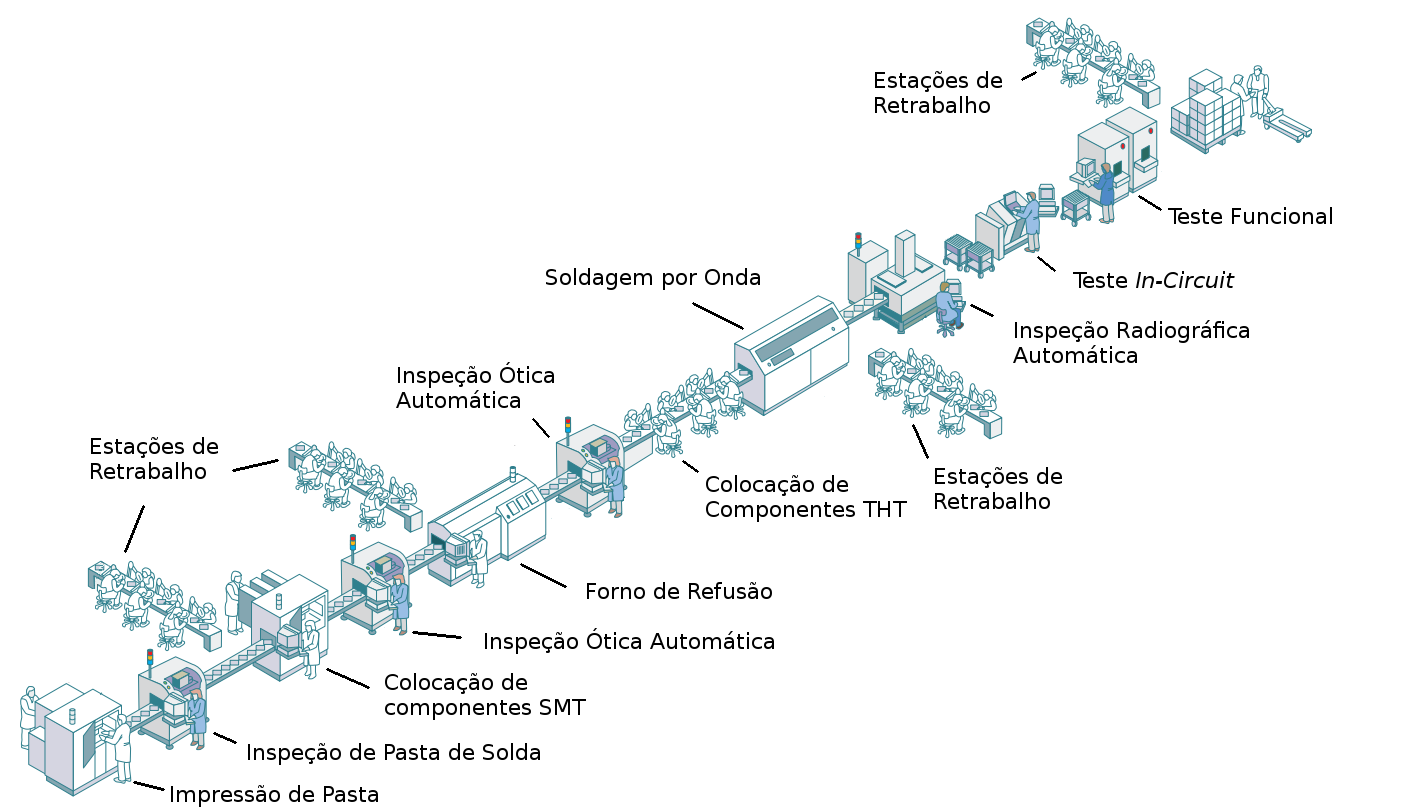
\includegraphics[width=1.1\linewidth]{linha.png}
    \caption{Uma típica linha de montagem de PCIs. Adaptado de \citet{agilenttechnologies2003}}
    \label{fig:linha}
\end{figure}


Juntamente com as métricas de cobertura de teste, os modelos de falta também cumprem um papel importante no estudo de testes de manufatura. \citet{jutman2014high} separa os modelos de falta nas seguintes classes: defeito materiais; defeitos em pinos e malha de circuito; problemas funcionais; e problemas de desempenho. 

Defeitos em materiais e mecânicos podem ser mensurados por métricas padrão de processo de qualidade e exemplificados por defeitos em placas, processo de montagem: solda ruim terminal levantado, componente defeituoso, desalinhamento, efeito lápide\footnote{Efeito Lápide, ou \textit{tumbstone effect}, é a elevação parcial ou total de componentes SMT passivos durante a refusão, assemelhando-se muitas vezes à uma lápide.}.

Os defeitos em pinos e malhas de circuito são modelados por análise estrutural e já possuem uma base bem estabelecida. Entram nessa classe as falhas de circuitos abertos ou em curto, defeito de driver (\textit{buffer}, pino).

Há ainda os problemas \textit{funcionais}, como falhas de \textit{boot}, cujas métricas são estabelecidas e investigadas por pesquisadores em desenvolvimento de software e lógica descritiva.
Por final, tem-se os problemas de desempenho em linhas de comunicação: alta taxa de erro, \textit{crosstalk, jitter, delay,} e outros.

Tradicionalmente na indústria, defeitos em materiais são solucionados durante a montagem da placa. Já os defeitos de pino, malha de circuito e funcional são testados no fim de linha de produção por duas categorias de teste denominados \textit{testes estruturais e testes funcionais}. A relação entre estas duas categorias de testes é descrita em  \citet{thomaswenzelenricozimmermann2016} e sintetizada na figura \ref{fig:cobertura}. Porém, em \citet{thomaswenzel2013} e \citet{jutman2014high}, nota-se que essa segmentação vem mudando com os avanços nas técnicas de verificação periférica e de teste centralizado por microcontrolador, que incorporam boa parte dos testes de desempenho e até mesmo funcionais. Tais técnicas serão descritas nas seção \ref{FCT} deste mesmo capítulo.

\begin{figure}[ht]
    \centering
    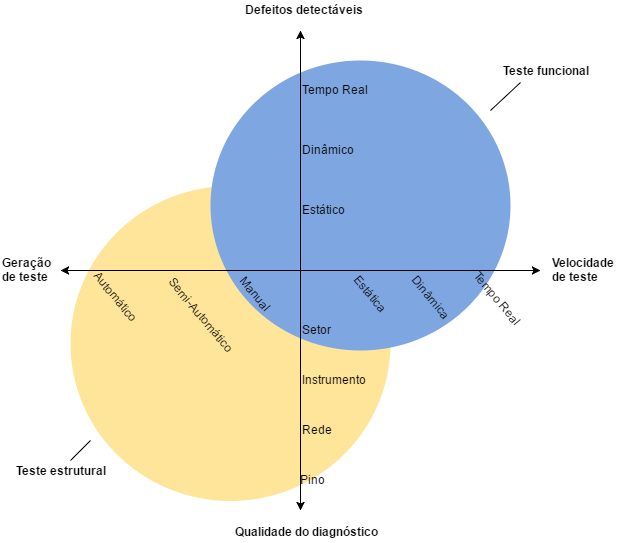
\includegraphics[width=1.0\linewidth]{complement.png}
    \caption{A complementariedade dos testes estruturais e funcionais para a cobertura de teste de um dispositivo. Adaptado de \cite{thomaswenzelenricozimmermann2016}.}
    \label{fig:cobertura}
\end{figure}

Viu-se aqui, portanto, que diversas técnicas e abordagens de teste e diagnóstico integram-se e são parte importante da produção, operação e manutenção de um sistema eletrônico. A seguir, estas técnicas serão descritas detalhadamente. 
\clearpage
\subsection{Inspeção de Pasta de Solda}

A inspeção de pasta de solda é o processo, normalmente automático, de achar falhas após a aplicação da pasta de solda. A inspeção de pasta de solda previne o retrabalho de placas com os componentes montados porque, uma vez com os erros de solda detectados, a placa defeituosa pode ser separada das demais. A detecção de falhas ainda nesta etapa custa 10 vezes menos do que uma falha pós refusão, ou após a solda, e 70 vezes menos que uma falha no teste elétrico intra-circuito (\textit{In-circuit test}) \citep{owen2000process}.

Os sistemas mais simples de inspeção de pasta de solda consistem de uma imagem colorida da placa. Este método consegue detectar ausência de solda e conexões indevidas entre blocos vizinhos, porém, por ser um método 2D, não consegue estimar a altura e volume da pasta de solda. Isso pode gerar problemas indetectáveis em outras etapas, já que, por mais que passe em testes de condutividade, a falta de pasta de solda em uma conexão pode causar problemas mecânicos e rompimento da interconexão. 

O volume de pasta de solda pode ser estimado por diversos métodos. \citet{5246351} introduz as principais tecnologias de perfilometria: 
\begin{itemize}
    \item Triangulação a laser;
    \item Perfilometria por fase, utilizando luz estruturada;
    \item Reconstrução por Redes Neurais.
\end{itemize}

Os métodos por triangulação a laser utilizam-se das projeções do feixe de laser no relevo da placa para reconstruir o seu perfil 3D.  \cite{5576321} descreve os detalhes desta técnica. Medições precisas podem ser obtidas com este método. Entretanto, são equipamentos caros, com baixa velocidade de inspeção, e susceptíveis a ruídos refletivos e \textit{efeito de sombras} \citep{5246351}.

Na perfilometria por fase, uma luz estruturada projeta um padrão, como uma grade ou uma série riscos, na PCI com a pasta de solda aplicada. Este padrão é então pouco a pouco deslocado e uma série de imagens são capturadas por uma câmera de alta resolução. Os sistemas mais avançados empregam um sistema livre de sombras onde ambos os lados da deposição de solda são caracterizados simultaneamente. \cite{5576321} oferece uma abordagem para o problema das sombras e \cite{5246351} faz uma revisão dos principais trabalhos em perfilometria por fase.

O método de reconstrução por redes neurais tenta resolver os problemas do \textit{shape-from-shading (SFS)}, que até então era um método cujo desempenho era inconsistente. \cite{5246351} revisa o estado da arte e propõe uma nova abordagem.

\subsection{Inspeção ótica automática - AOI}
% inserir https://repositorio.ufsc.br/xmlui/bitstream/handle/123456789/158843/337436.pdf?sequence=1&isAllowed=y

A inspeção ótica automática (AOI), como o próprio nome indica, inspeciona visualmente a placa de circuito por meio de fotos, processa e identifica automaticamente as falhas, seja de componente ou solda. Esta técnica é usada para detectar componentes trocados, faltantes ou mal posicionados e pode ser realizada na etapa pré-forno de refusão ou após, dependendo da particularidade do processo produtivo da fábrica. O trabalho de \cite{huang2015automated}, citado por \cite{mello2015sistema}, indica quatro categorias de inspeção ótica automática:

\begin{itemize}
    \item \textbf{Métodos de projeção}, que correlacionam a entrada com modelos aprendidos e suas características;
    \item \textbf{Abordagem baseada em filtro:} filtro espaciais com base em transformadas de sinal, como por exemplo, Fourier, Wavelet, discreta cosseno;
    \item \textbf{Aprendizagem de máquinas:} Os mais utilizados são as redes neurais, algoritmos genéticos, e máquinas de vetor suporte;
    \item \textbf{Abordagens híbridas:} associam diversas técnicas para classificações mais complexas. 
\end{itemize}

%A AOI na etapa pré-forno detecta componentes faltantes ou componentes errados, e alinhamento correto de componentes. Como este processo é realizado após a refusão, os defeitos são relativamente simples de corrigir e menos custosos do que após a etapa de refusão. Outra vantagem é que os problemas de calibração na máquina de posicionamento de componentes podem ser mais facilmente detectados e analisados. Uma análise de tendência nas etapas pós refusão não seria tão confiável, pois o processo de refusão altera a localização dos componentes, e problemas de calibração na máquina de posicionamento só seriam detectados após um aumento significativo de placas defeituosas.

%Na etapa pós refusão, a inspeção ótica automática é provavelmente a etapa mais aceita entre os fabricantes de placas eletrônicas. Um sistema AOI colocado nesta etapa detecta qualquer problema gerado ao longo do processo, incluindo defeitos de colocação de componentes e problemas relacionados à solda, como: falta ou excesso de solda, curto-circuitos ou circuitos abertos. Nesta etapa, a AOI detecta defeitos causados por problemas de impressão, pelo sistema de colocação de componentes, e ainda, pelo processo de refusão. O propósito da AOI após o processo de refusão não é somente prover dados de defeito necessários para o retrabalho de uma PCI, mas também para a coleta de dados através de múltiplas montagens de placa para análise de causa raíz e melhoramento contínuo da produção.

A maior limitação da AOI é a impossibilidade de detecção de defeitos em pinos ou partes do circuito não visíveis, como abaixo de componentes \textit{Ball Grid Array} (BGA) ou em circuitos eletromagneticamente blindados. Nesses casos, é necessário o uso de outras ferramentas, como a verificação de placas por radiografia.
%\cite{savage1993automated} citado por \citep{mello2015sistema}
%todo
\subsection{Inspeção radiográfica automática - AXI}

A inspeção radiográfica automática (AXI) possui uma vantagem única em relação às outras tecnologias de inspeção estrutural: os materiais absorvem os raios-x proporcionalmente à sua massa atômica. A solda utilizada na montagem das PCIs consiste de materiais pesados como o chumbo e a prata. A maioria restante dos materiais usados na fabricação das PCIs é composta por elementos leves como carbono, silício, alumínio, oxigênio, hidrogênio e cobre. Dessa forma, a inspeção radiográfica mostra-se muito interessante na geração de imagens do processo de solda: os pontos de solda aparecem muito bem, enquanto o restante da placa apresenta-se transparente. Outra vantagem é a possibilidade de inspecionar os pinos escondidos de encapsulamentos complexos como o BGA ou o \textit{chip-scale packages} (CSP), além de exibir características internas dos pontos de solda.

\subsubsection{Tipos de AXI}

 As técnicas AXI utilizadas em processos de manufatura e diagnóstico se dividem entre bidimensional e tridimensional \citep{7236817, dougmcclure2000}. 

A inspeção 2D é semelhante à radiografia convencional, porém com recursos de visão computacional para análise automática. É melhor aplicada em placas com soldas em um só lado da placa. Em placas com junções de solda em alta densidade ou em ambos os lados, a imagem gerada pode ficar confusa. 

Com a laminografia e tomografia computadorizada é possível obter a imagem de um recorte da placa e, associada a técnicas de processamento digital, reconstruir um modelo tridimensional da placa. A laminografia utiliza-se do movimento do emissor e detector que pode ser rotacional \citep{7236817} ou linear \citep{6756131}. A desvantagem da radiografia tridimensional é o tempo necessário para a captura da imagem e seu processamento \citep{6756131}. 

\subsubsection{Casos onde a inspeção radiográfica é importante}

\citet{leinbach2001and} apresenta três casos aonde a inspeção radiográfica se faz importante. Primeiro, na inspeção de componentes visualmente ocultos, como terminais de encapsulamentos CSP e BGA ou componentes sob blindagem RF. Segundo, em aplicações que exigem alta qualidade de solda, como as PCI expostas a ambientes de estresse mecânico ou térmico. Terceiro, em projetos de PCI complexos, cujas taxas de erro de produção por placa são mais frequentes e a AXI consegue garantir o rigor do processo de inspeção.

\citet{7236817} faz um estudo comparativo entre tecnologias de inspeção radiográfica para detecção de defeitos em furos galvanizados. \citet{7428398} aplicou AXI na inspeção de componentes \textit{press-fit} e \citet{7428400} na verificação do resinamento de placas de circuito impresso montadas. Combinada com técnicas de ICT, a maior parte dos defeitos podem ser cobertos. O trabalho de \citet{oresjo2002use} comenta melhor a relação entre AOI, AXI, e os testadores intra-circuito (\textit{in-circuit testers - ICT}).

\subsection{Testes intra-circuito (\textit{In-Circuit Testers - ICT)}}

Jigas de teste são uma grande ferramenta de teste de placas de circuitos eletrônicos. Por meio de pontas de teste, pode-se obter acesso a pontos internos do circuito, como também, testar componentes isoladamente, separando-os de outros circuitos. Por meio de ICT, é possível detectar componentes defeituosos ou faltantes, circuitos abertos ou em curto e, até mesmo, componentes errados. O ICT trabalha testando partes isoladas da placa, medindo resistência, capacitância e, em alguns casos, indutância de subcircuitos da placa, normalmente acessíveis por conectores, pads, ou \textit{test points}. Dessa forma, consegue-se realizar testes estruturais e até mesmo funcionais sobre o circuito, garantindo que sua fabricação foi correta e que se encontra funcional. Muitas vezes, o ICT é usado também para a gravação de \textit{firmware} nas placas. Os ICT são compostos pelos seguintes elementos \citep{ianpoole2017}:

\begin{itemize}
    \item O ICT em si: composto por uma matriz de pares de acionadores e sensores que são usados para realizar as medições. Podem ser em torno de centenas, ou até milhares, por ICT.
    \item A jiga de teste (\textit{fixture} ou fixação):  é a interface entre o ICT e a placa testada, roteando as entradas e saídas do ICT com o Dispositivo em Teste, através de pinos, num arranjo conhecido como cama de pregos.
    \item O software de teste: software com a rotina de testes e condições de aprovação/reprovação.
\end{itemize}

Dentre os três, somente o ICT em si não é customizado para cada placa. O sistema de jiga de testes, por ser relativamente caro, é mais bem aplicado a grandes volumes de produção. Uma análise de custos deve de ser realizada para garantir que os custos de montagem da jiga e do programa sejam viáveis. 

\subsubsection{Tipos de ICT}

A tabela \ref{table:tiposdeict} sintetiza três categorias principais de testadores \citep{ianpoole2017}: O ICT tradicional; O \textit{flying probe test - FPT}, cujas pontas de prova são controladas por comando numérico computadorizado (CNC); e o Analisador de Defeito de Fabricação: versão mais enxuta do ICT, com funcionalidades reduzidas. 

\begin{table}[h!]
\centering
\caption{Tipos de ICT}
\label{table:tiposdeict}
{\footnotesize 
\begin{tabularx}{\textwidth}{@{} Y Y Y Y @{}}
\toprule
  \textbf{Tipo de ICT} & \textbf{Princípio de \mbox{Funcionamento}}  &\textbf{Vantagens}  &\textbf{Desvantagens} & \\ \midrule
\textbf{ICT tradicional} & - Pares de I/O em grande número; 

- Fixação e cama de pregos feitos sob medida. & - Alta velocidade de execução de teste; 

- Capacidade para medição de capacitância e indutância. & - Inviável para pequenas produções;

- Custo adicional para qualquer atualização da jiga;  \\ \addlinespace
\textit{\textbf{Flying probe test (FPT)}} & - Pontas de prova móveis e controladas por CNC; 

- A fixação de placa é genérica;
 & - Dispensa uma jiga de teste e cama de pregos; 
 
 - Alterações realizadas via software;
 & 
- Número limitado de pontos de testes simultâneos; 

- Baixa velocidade de teste; & \\ \addlinespace
\textbf{Analisador de Defeitos de Fabricação}
 & - Similiar ao ICT padrão, mas com funções limitadas.
 & - Alta velocidade de teste e custo reduzido;
 & - Limita-se a testes de continuidade e resistência elétrica.
  & \\ \bottomrule
\end{tabularx}}
\end{table}

\subsubsection{Cobertura de falta}
Em sua tese, \citet{de2008apoio} relata que os testes funcionais e estruturais realizados por ICT foram progressivamente dificultados por duas questões. 

A primeira é a miniaturização dos circuitos e componentes com valores muito baixos, cuja verificação é comprometida  devido à influência de capacitâncias parasitas do próprio testador. O mesmo acontece com as indutâncias mas, ao menos, é possível detectar a presença do componente ao medir a resistência entre os terminais.

O segundo problema, e também o mais grave, é relacionado ao acesso aos nós do circuito, seja pelas dimensões reduzidas da placa sob teste, que dificultam a construção de uma cama de pregos correspondente, como também pela completa inacessibilidade a uma região eletromagneticamente blindada ou a pinos inacessíveis de encapsulamentos de alta densidade, como os BGAs, que, hoje em dia, estão quase sempre presentes em placas de circuito impresso.

Estes fatores deram origem ao desenvolvimento da infra-estrutura normatizada de circuitos de varredura periférica IEEE 1149.1 \citep{ieee11491old} para facilitar o teste de integrados digitais que, nas ultimas décadas, expandiu-se em outros padrões que cobrem desde medições analógicas a testes de canais de comunicação. 

\subsection{Varredura periférica}

Testes de varredura periférica (\textit{boundary scan}) como o \textit{Joint Test Action Group - JTAG} são hoje o padrão da indústria em teste de placas de circuito impresso e vem, ao longo dos últimos anos, substituindo os ICT. Isso se deve ao custo baixo desta tecnologia e eficiência em termos de cobertura de testes. Os primeiros esforços para a criação de um padrão de varredura periférica ocorreram na década de 80 e foram encabeçados pelo \textit{Joint Test Action Group - JTAG}, cujo trabalho se consolidou no padrão \citet{ieee11491old}, que obteve rápida adoção pela indústria eletrônica. Sua revisão mais atual é a \citet{ieee11491yr2013}.
A necessidade de um padrão de varredura periférica surgiu devido aos crescentes custos e dificuldades na criação de jigas de teste para ICTs, principalmente pelo aumento da densidade de componentes e pela falta de espaço para a inserção de pontos de teste no leiaute de circuito impresso, como também, por causa da distribuição de componentes em ambas as superfícies. 

Embora as primeiras aplicações do JTAG fossem direcionadas para teste de placas de circuito impresso, hoje o padrão também cumpre um papel essencial na depuração de sistemas embarcados, graças ao acesso de baixo nível às entradas/saídas e estados internos do circuito integrado, fornecendo um meio barato e confiável de depuração.
A porta JTAG também serve para a gravação de \textit{firmware} na memória flash \citep{ieee1532}, sendo uma alternativa mais rápida ao uso de portas seriais e \textit{bootloaders}. 

Outra aplicação desta interface é a geração de testes automatizados para diagnóstico de placa em campo no conceito de BIST, ou auto teste embutido, possibilitando que uma placa faça auto-diagnóstico de problemas, como em circuitos periféricos. Estes conceitos serão abordados no próxima seção deste trabalho.

\begin{figure}
    \centering
        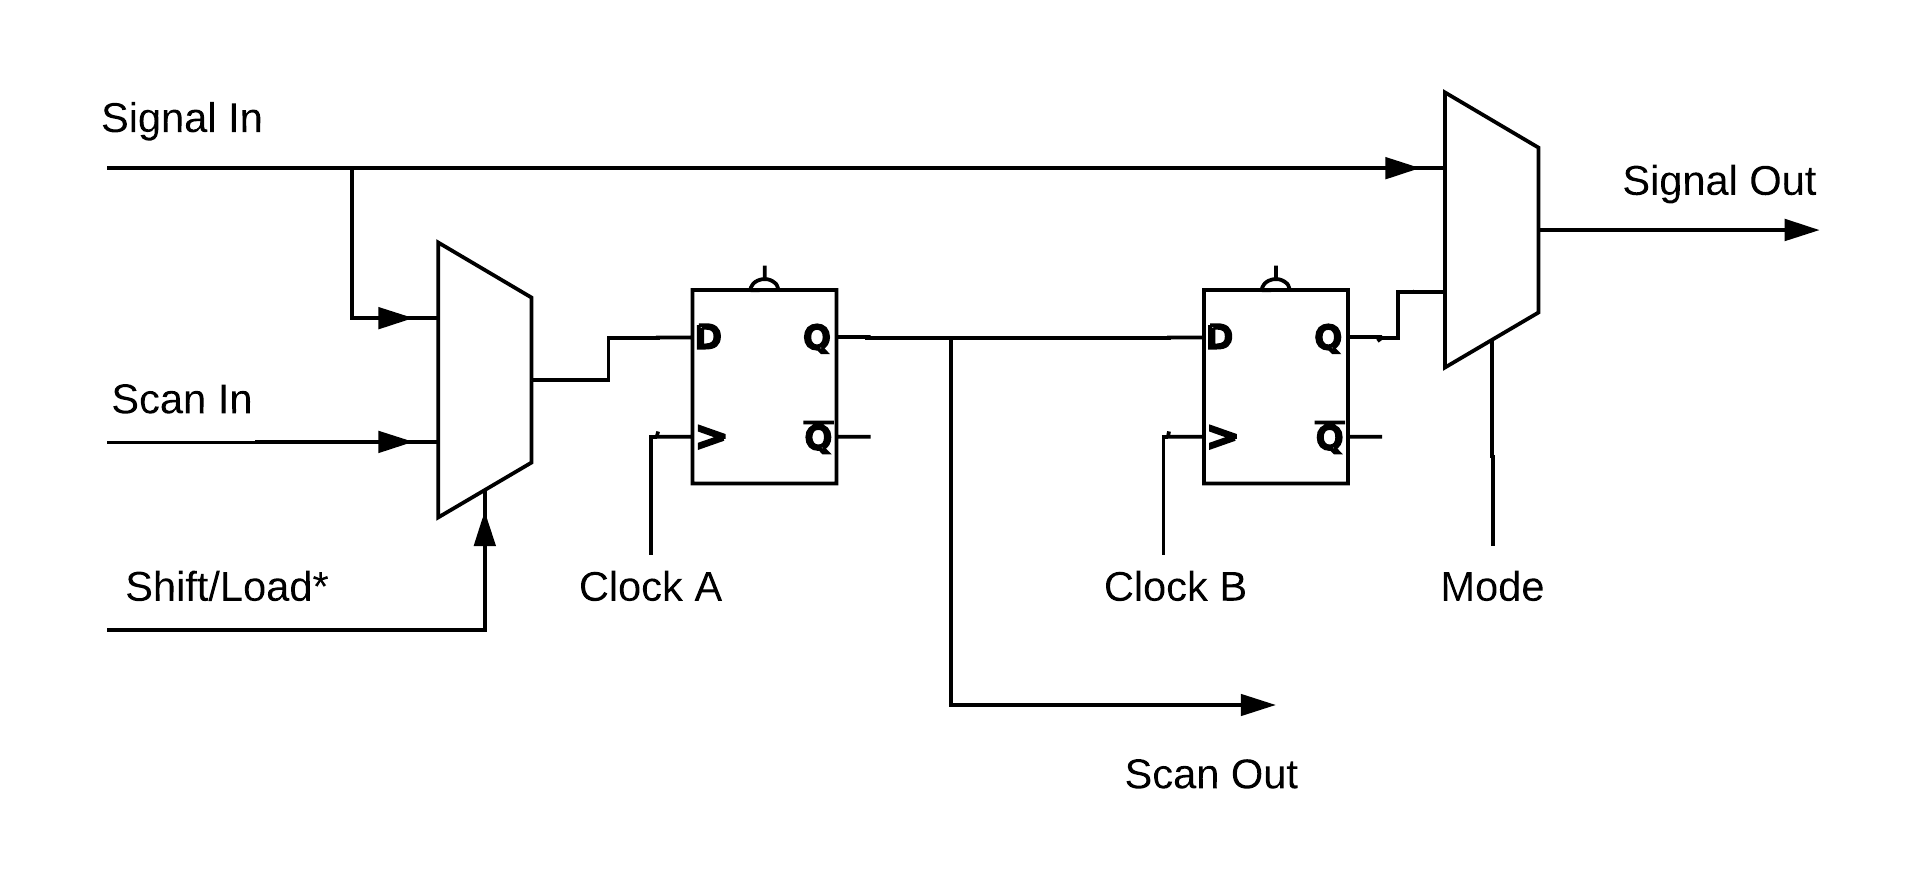
\includegraphics[width=0.8\linewidth]{fig/bscell}
            \caption{Célula de Verificação Periférica}
            \label{fig:bscell}
\end{figure}


O padrão IEEE 1149.1 se baseia em células de teste embutidas em todos os pinos de E/S do circuito integrado (figura \ref{fig:bscell}). As células são encadeadas em uma topologia em anel, um esquema conhecido como \textit{daisy-chain}. O gerenciamento da cadeia de verificação é realizado pela porta de acesso ao teste (ou, em inglês, \textit{test acess port - TAP}), permitindo que todos os pinos de E/S do circuito integrado sejam acessíveis e testados pela porta JTAG. A figura \ref{fig:tap} mostra o esquemático conceitual da lógica interna da porta JTAG. A conexão em \textit{daisy-chain} entre os pinos de um dispositivo com suporte ao IEEE 1149.1 pode facilmente ser estendida para outros integrados compatíveis com o padrão, possibilitando o teste de múltiplos circuitos integrados através de um único conector (figura \ref{fig:cadeiabs}). Como boa prática de DfM, recomenda-se a escolha de integrados que atendam ao padrão.

\begin{figure}
    \centering
        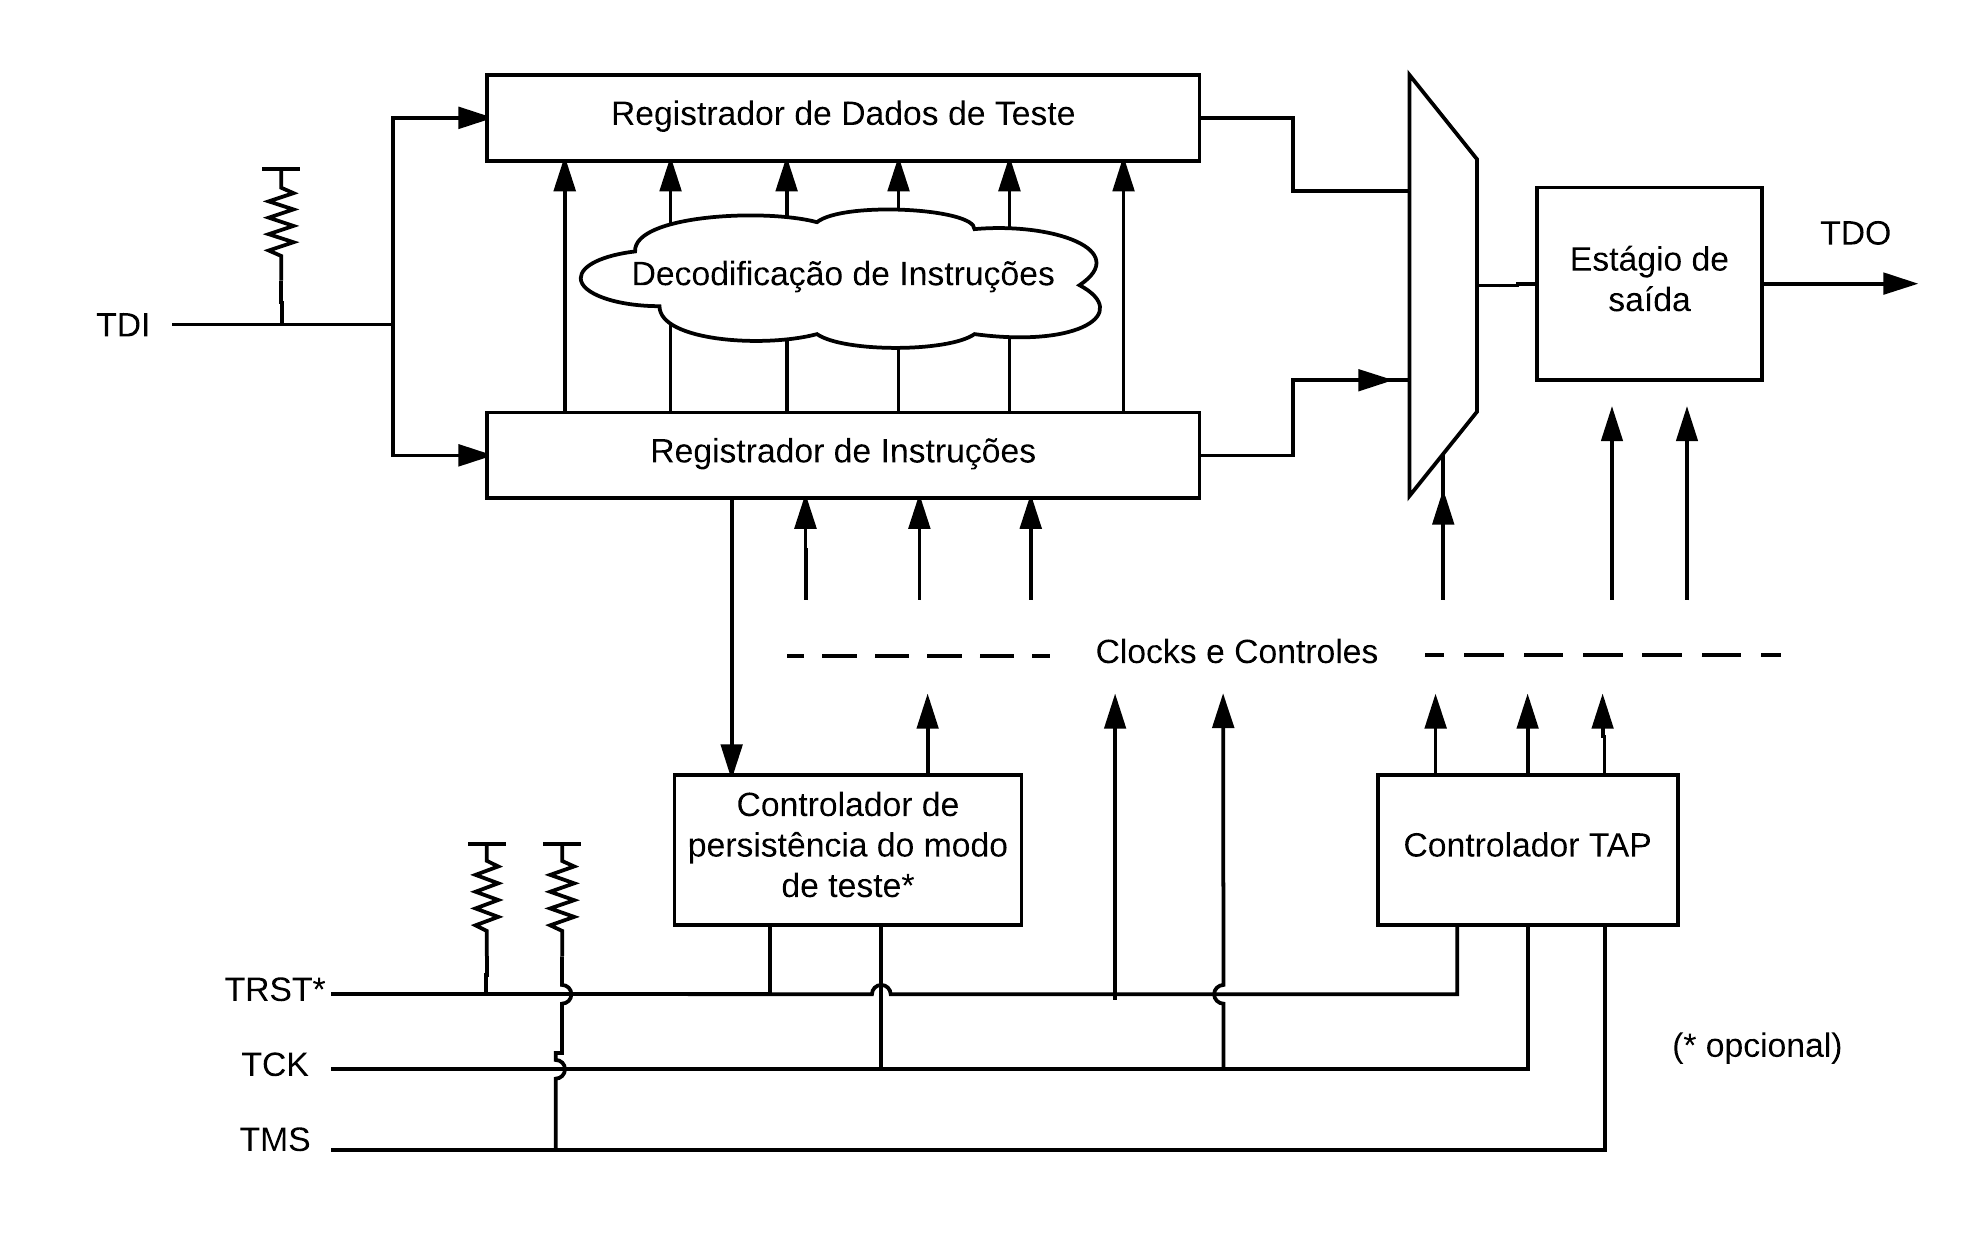
\includegraphics[width=1.0\linewidth]{fig/TAP}
            \caption{Esquemático conceitual da lógica de teste \textit{on-chip}}
            \label{fig:tap}
\end{figure}

Outro componente importante do JTAG é a linguagem de descrição de varredura periférica (BSDL em inglês), que foi inserida numa revisão posterior do IEEE 1149.1 \citep{ieee11491de94}. A BSDL é um subconjunto do VHDL e é voltada para a descrição da infraestrutura de teste de um CI com o objetivo de tornar mais consistente a geração de testes e toda a cadeia de desenvolvimento envolvida nisso.

\begin{figure}
    \centering
        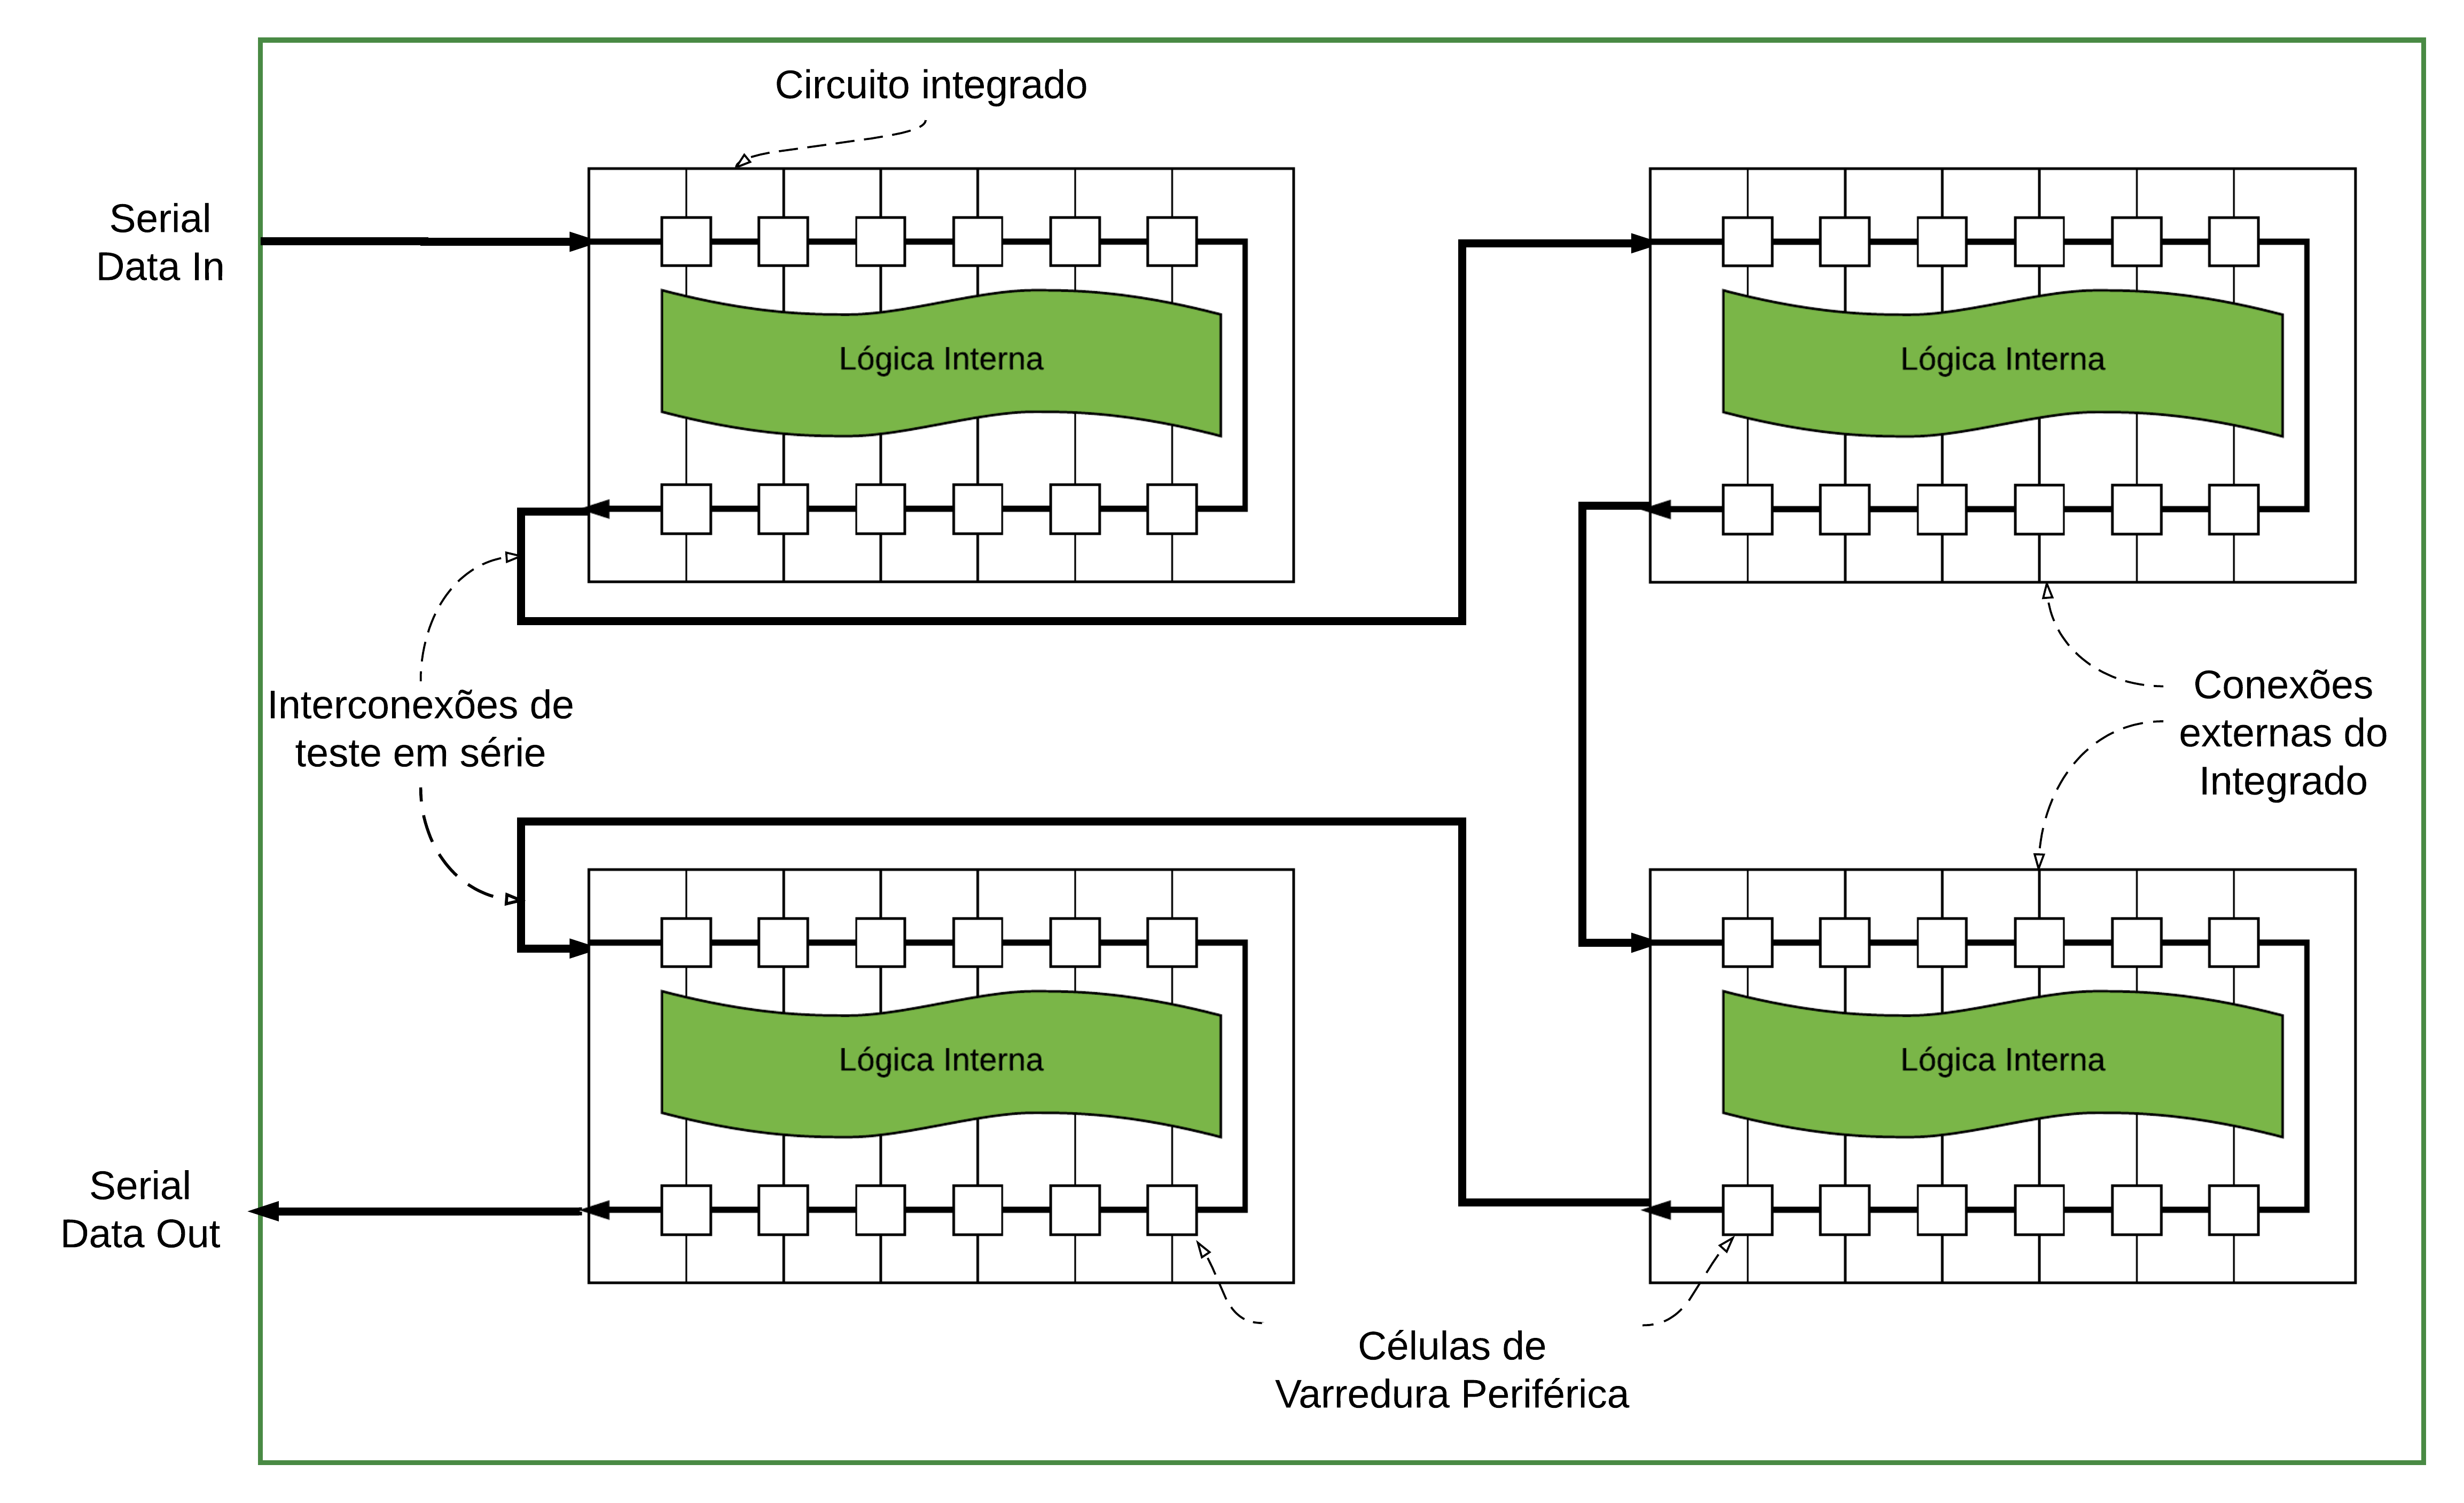
\includegraphics[width=1.0\linewidth]{fig/cadeiabs}
            \caption{PCI com as portas JTAG em \textit{daisy-chain}}
            \label{fig:cadeiabs}
\end{figure}


O padrão IEEE 1149.1 serviu de base para a criação de uma família de padrões de varredura periférica, que são exibidos na tabela \ref{tab:boundaryscanfamily} - adaptada de \citet{jutman2014high}.  

\begin{table}[h]
\centering
\tiny
\caption{Padrões IEEE de varredura periférica \citep{jutman2014high}}
\label{tab:boundaryscanfamily}
\begin{tabular}{p{50}p{50}p{50}p{50}}
\hline
\rowcolor[HTML]{C0C0C0} 
\multicolumn{1}{|p{50pt}|}{\cellcolor[HTML]{C0C0C0}\textbf{Foco principal de aplicação}} & \multicolumn{1}{p{50pt}|}{\cellcolor[HTML]{C0C0C0}\textbf{Propósito Principal}} & \multicolumn{1}{p{50pt}|}{\cellcolor[HTML]{C0C0C0}\textbf{Base da Tecnologia}}    & \multicolumn{1}{p{50pt}|}{\cellcolor[HTML]{C0C0C0}\textbf{Classes de falta a serem cobertas}}     \\
\rowcolor[HTML]{656565} 
\multicolumn{4}{|l|}{\cellcolor[HTML]{656565}{\color[HTML]{FFFFFF} \textbf{IEEE 1149.1 - Boundary Scan \citep{ieee11491old, ieee11491yr2013}}}}                                                                                        \\
\multicolumn{1}{|p{50pt}|}{Teste de Manufatura de PCI}                                        & \multicolumn{1}{p{50pt}|}{Melhorias de acesso aos testes}                               & \multicolumn{1}{p{50pt}|}{Registradores de sondagem on-chip}                            & \multicolumn{1}{p{50pt}|}{Faltas em pinos e integridade de circuto}                                 \\
\rowcolor[HTML]{656565} 
\multicolumn{4}{|l|}{\cellcolor[HTML]{656565}{\color[HTML]{FFFFFF} \textbf{IEEE 1149.4 - Barramento para testes de sinais mistos \citep{ieee11494}}}}\\

\multicolumn{1}{|p{50pt}|}{Medição de sinais analógicos} &
\multicolumn{1}{p{50pt}|}{Melhorias de acesso aos testes} & 
\multicolumn{1}{p{50pt}|}{Chaves \textit{on-chip}} &
\multicolumn{1}{p{50pt}|}{Valores paramétricos}\\

\rowcolor[HTML]{656565} 
\multicolumn{4}{|l|}{\cellcolor[HTML]{656565}{\color[HTML]{FFFFFF} \textbf{IEEE 1149.6 - Teste BST de Redes Digitais Avançadas \citep{ieee11496}}}}\\

\multicolumn{1}{|p{50pt}|}{Teste de redes LVDS de alta velocidade} &
\multicolumn{1}{p{50pt}|}{Teste de malhas acopladas em corrente alternada} & 
\multicolumn{1}{p{50pt}|}{Geradores de pulsos \textit{on-chip}} &
\multicolumn{1}{p{50pt}|}{integridade de malha}\\

%\rowcolor[HTML]{656565} 
\multicolumn{4}{|l|}{\cellcolor[HTML]{656565}{\color[HTML]{FFFFFF} \textbf{IEEE 1149.7 - Pinos reduzidos e TAP aprimorado \citep{ieee11497}}}}\\

\multicolumn{1}{|p{50pt}|}{Teste de placa e depuração de software} &
\multicolumn{1}{p{50pt}|}{Acesso à teste flexivel e em alta velocidade por dois pinos} & 
\multicolumn{1}{p{50pt}|}{SERDES, endereçamento} &
\multicolumn{1}{p{50pt}|}{Contempla todos acima}\\

%\rowcolor[HTML]{656565} 
\multicolumn{4}{|l|}{\cellcolor[HTML]{656565}{\color[HTML]{FFFFFF} \textbf{IEEE 1149.8.1 - Alternância de pinos e sensoriamento sem contato\citep{ieee114981}}}}\\

\multicolumn{1}{|p{50pt}|}{Teste de interconexão de PCIM} &
\multicolumn{1}{p{50pt}|}{Ligações para componentes passivos} & 
\multicolumn{1}{p{50pt}|}{chapas de sensoriamento capacitivo} &
\multicolumn{1}{p{50pt}|}{Circuitos abertos: AC e DC }\\

\multicolumn{4}{|l|}{\cellcolor[HTML]{656565}{\color[HTML]{FFFFFF} \textbf{IEEE P1149.10- TAP de alta velocidade \citep{ieeep1149102016} }}}\\

\multicolumn{1}{|p{50pt}|}{O mesmo que todos acima} &
\multicolumn{1}{p{50pt}|}{Permutação de dados de teste em alta velocidade} & 
\multicolumn{1}{p{50pt}|}{Reuso de pinos I/O de alta velocidade} &
\multicolumn{1}{p{50pt}|}{O mesmo que todos acima}\\

\multicolumn{4}{|l|}{\cellcolor[HTML]{656565}{\color[HTML]{FFFFFF} \textbf{IEEE 1500 - Teste de núcleo embarcado \citep{ieee1500}}}}\\

\multicolumn{1}{|p{50pt}|}{Teste à nível de SoC e IP} &
\multicolumn{1}{p{50pt}|}{Acesso ao teste de \textit{IP cores} em um SoC} & 
\multicolumn{1}{p{50pt}|}{invólucros de núcleos} &
\multicolumn{1}{p{50pt}|}{Faltas no domínio digital dentro de um CI}\\

\multicolumn{4}{|l|}{\cellcolor[HTML]{656565}{\color[HTML]{FFFFFF} \textbf{IEEE 1687 - Acesso por Instrumentação Embarcada \citep{ieee1687}}}}\\

\multicolumn{1}{|p{50pt}|}{Teste de CI, depuração, diagnóstico} &
\multicolumn{1}{p{50pt}|}{Padrão de acesso por instrumento} & 
\multicolumn{1}{p{50pt}|}{Cadeias de sonda reconfiguráveis} &
\multicolumn{1}{p{50pt}|}{Específicas do instrumento}\\

\multicolumn{4}{|l|}{\cellcolor[HTML]{656565}{\color[HTML]{FFFFFF} \textbf{IEEE P1838 - Acesso a teste para CIs 3D \citep{ieeep18382016}}}}\\

\multicolumn{1}{|p{50pt}|}{Teste de integração 3DSIC} &
\multicolumn{1}{p{50pt}|}{Acesso à teste através das vias TSV} & 
\multicolumn{1}{p{50pt}|}{O mesmo que os padrões 1500, 1149.1, 1687} &
\multicolumn{1}{p{50pt}|}{Integridade das vias TSV}\\
\hline


\end{tabular}
\end{table}

O padrão IEEE 1149.4 \citep{ieee11494} foi criado para testes paramétricos de componentes passivos, resistores pull-ups, componentes ativos como diodos, transistores e de redes de impedância. Serve como uma extensão da varredura periférica para sinais analógicos. Este padrão ainda tem um número limitado de dispositivos compatíveis.

Já o padrão IEEE1149.6 \citep{ieee11496} estende a varredura periférica a portas de comunicação com acoplamento em corrente alternada, como por exemplo, portas que atendem ao padrão de LVDS, operando em paralelo com os padrões 1149.1 e 1149.4. O que possibilita esta tecnologia são as inserções de geradores de pulso nos pinos de saída e \textit{receivers} CA comuns e diferenciais nas entradas dos dispositivos que dão suporte a este padrão.

É possível citar outros exemplos significativos, como é o caso do IEEE1149.7 - cJTAG \citep{ieee11497}. Este padrão opera em pinos reduzidos e possibilita uma topologia em estrela ao invés do \textit{daisy-chain}, permitindo um acesso mais rápido, além de oferecer uma infraestrutura adicional de suporte a tecnologias mais avançadas. O IEEE P1687 \citep{ieee1687} introduz o conceito de instrumentação embarcada para a aplicação de tarefas de teste, medição e diagnóstico, assunto abordado na próxima seção.

\subsection{Teste Controlado por FPGA ou Processador e Instrumentação Embarcada}
\label{FCT}

Conforme mencionado anteriormente, o JTAG não permite o uso de padrões de teste em velocidade nominal, deixando a classe de falhas de desempenho sob responsabilidade de testes funcionais. Atualmente, parte da indústria tem utilizado os componentes centrais de seus sistemas, como por exemplo os FPGAs e microcontroladores, como dispositivos de teste embarcado \citep{alcrouch2011, thomaswenzel2013}, cunhando os termos \textit{FPGA-Controlled Test - FCT} e \textit{Processor-Controlled Test - PCT}. 

 Além de cobrir os testes em domínio CA, como atrasos e \textit{crosstalk}, ainda possibilitam um acesso de baixo nível no sistema, já que esses são normalmente componentes centrais do projeto. O custo marginal é ínfimo, já que o todo o hardware de teste é reutilizado do produto e a memória de teste é apagada, voltando o dispositivo para sua funcionalidade original. \citet{jutman2014high} afirmou que ainda são poucas as empresas que fornecem ferramentas automatizadas para esta classe de testes.

O conceito de teste controlado por FPGA é possibilitado pelo uso de instrumentos embarcados, que são definidos como qualquer estrutura lógica dentro de um dispositivo cuja função é de teste, diagnóstico, \textit{Design for Testability (DfT), Design for Debug  (DfD), Design for Yield (DfY),} e outros. Neste escopo, enquadram-se diversas estruturas lógicas:    
\begin{itemize}
    \item Testadores de memória e BIST/BISD;
    \item Analisadores de taxa de erro (BERT) em canais de comunicação;
    \item Geradores de padrões de teste e \textit{buffers} de captura digital;
    \item Caracterizadores e Calibradores de E/S complexas;
    \item Testadores de barramentos de comunicação LAN, SATA, PCI, CAN, LIN, I2C, SPI e UART;
    \item Testadores sistêmicos e programação de memórias não voláteis;
    \item Instrumentos definidos por usuário.
\end{itemize}

\citet{Stollon2011} mostra que estas estruturas de instrumentação embutida surgiram, em parte, pela necessidade de medições que causem menos interferências ou que não comprometam a integridade do sinal de barramentos de alta velocidade, internos ou externos ao CI. Dessa forma, os fabricantes passaram a embutir núcleos de propriedade intelectual - \textit{IP cores} - de instrumentação interna, permitindo testes não intrusivos e facilitando a validação e diagnóstico de placas.

Originalmente, cada um destes instrumentos são acessados e gerenciados por uma variedade de instrumentos externos, usando diversos mecanismos e protocolos. Isso dificulta a integração entre CIs e o reuso de tecnologia e equipamento. Logo, existia uma necessidade de padronização destes protocolos, de forma a garantir uma metodologia eficiente e organizada para a preparação de testes e para o acesso e controle destes instrumentos embarcados. 

O IEEE 1687 \citep{ieee1687}, também conhecido como \textit{Internal JTAG } ou IJAG, foi o padrão criado para definir e descrever as interfaces de acesso à instrumentação embarcada pela porta padrão IEEE1149.1, possibilitando a realização de testes avançados e não intrusivos em uma PCI inteira pela porta JTAG. Como ilustrado na figura \ref{fig:ieee1687}, o IJTAG não define os instrumentos ou suas funcionalidades por si, mas sim os padrões de infraestrutura de acesso e como descrever os métodos e funcionalidades dos instrumentos. Isso se consolidou em duas linguagens de descrição dentro deste padrão: uma para as características destas funcionalidades, a PDL \textit{(procedural description language)}, e outra para os requerimentos de interface com estas funcionalidades - ICL \textit{(instrument connectivity language)}. Estas duas linguagens de descrição - PDL e ICL - facilitam o reuso e a descoberta de qualquer instrumento que seja compatível com o padrão IEEE 1687, independente do seu tipo, propósito ou origem. 

\begin{figure}
    \centering
        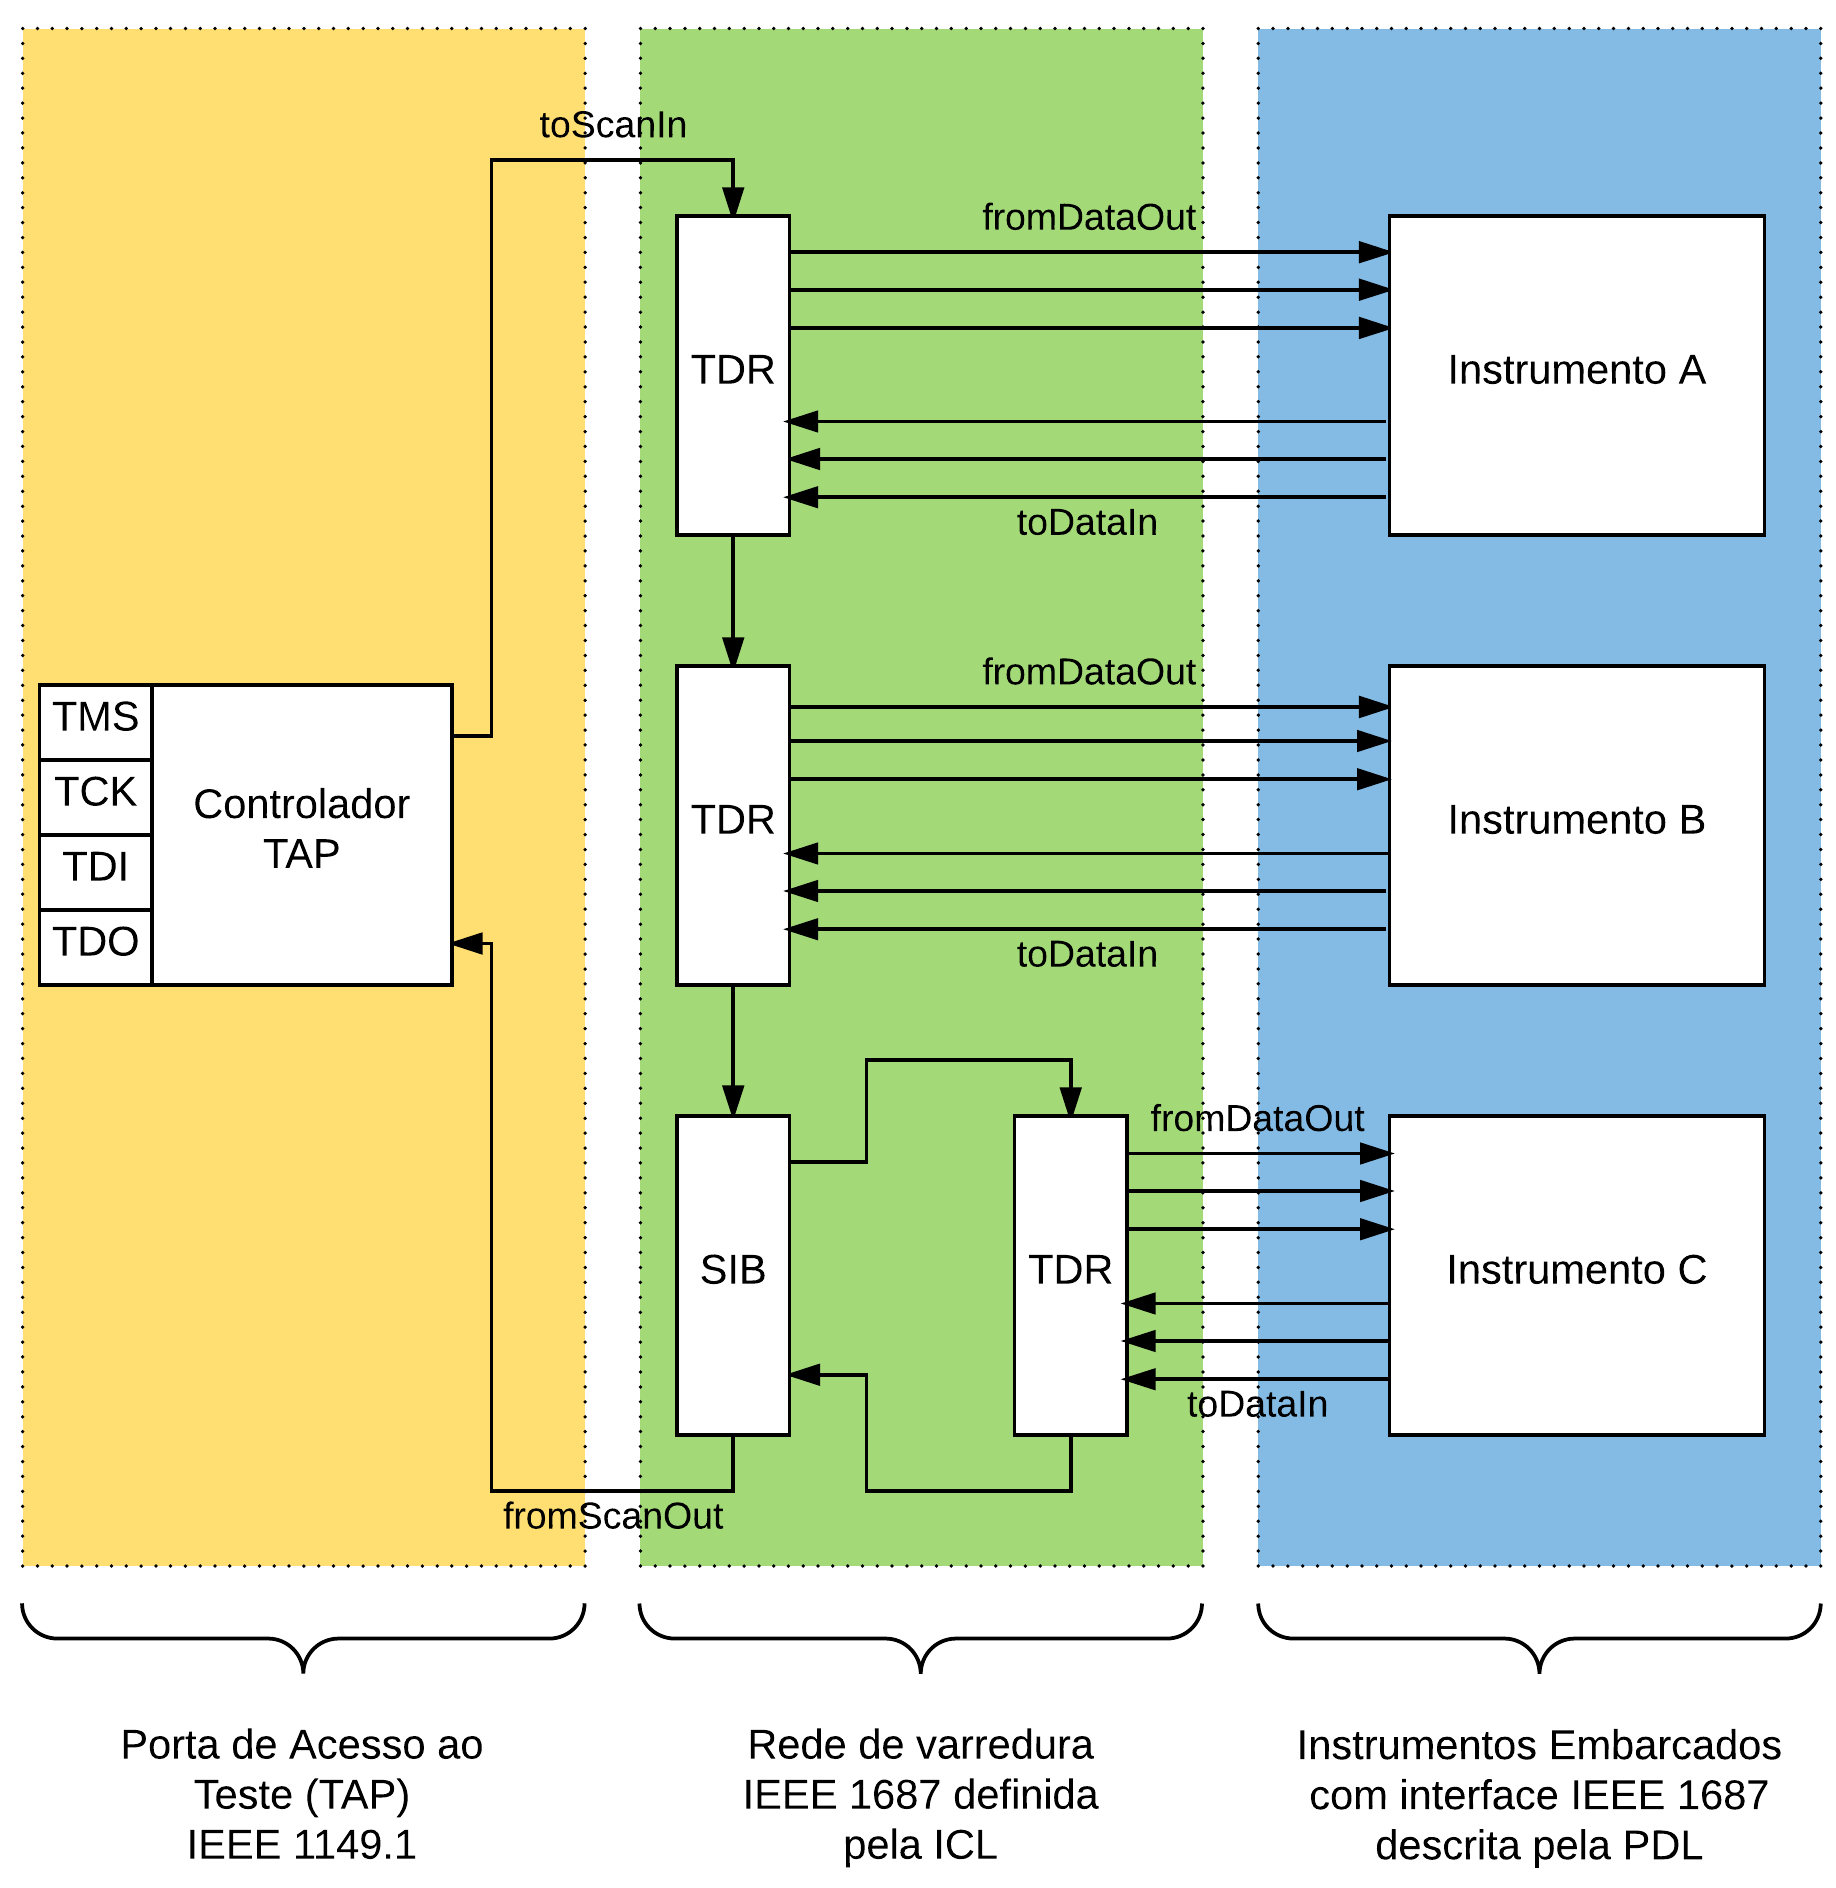
\includegraphics[width=1.0\linewidth]{fig/IEEE1687}
            \caption{Rede IEEE 1687 conceitual de múltiplas cadeias de varredura}
            \label{fig:ieee1687}
\end{figure}

Dessa forma, o padrão IEEE 1687 funciona como uma extensão do IEEE 1149.1, de maneira que a porta JTAG de um CI ou uma placa possa ser usada para configurar, operar, e coletar dados de instrumentos embarcados.

Os FCT e PCT aliados ao IEEE 1687 oferecem uma cobertura em múltiplos domínios de falta (estruturais, CC, CA e faltas de desempenho), reduzindo ou até mesmo superando a necessidade de equipamentos de teste especializados \citep{thomaswenzel2013}. Em \citet{jutman2014high} observa-se que isso possibilita não só uma manufatura e teste de produção mais baratos e descomplicados, como também abre porta para o reuso dos testes em campo para o diagnóstico de falhas operacionais, o que não só reduz os custos logísticos de transporte de equipamentos especializados para depuração e diagnóstico, como possibilita que testes avançados sejam realizados sob condições reais de operação. 

\subsection{Teste Funcional}
% https://pad.riseup.net/p/RwPsE9imTtNzadskjasdoqidjefkadf
%definição
Define-se teste funcional como aquele que não depende da estrutura interna de DfT de um sistema, mas sim das portas de entrada e saída \citep{jutman2014high}. Outra definição, formulada pelo mesmo autor, é a de um teste que se baseia somente nas informações funcionais do sistema, sem conhecimento da estrutura interna. Essas duas definições se interseccionam na maioria das vezes.

% APLICAÇÕES
% quero dizer que em todos autores é unanime que
O teste funcional serve para complementar objetivos específicos de teste, sendo normalmente empregado como etapa final de linha de produção \citep{thibeault2006,jutman2014high,tumim2001}. A tendência é que o teste funcional, devido aos seus custos crescentes, perca espaço com a adesão e popularização dos padrões mais avançados de varredura periférica e instrumentação embarcada, limitando-se a atingir certos objetivos específicos de teste que não podem ser cobertos por testes de varredura \citep{thibeault2006, thomaswenzelenricozimmermann2016}. 

Entretanto, existem casos onde o suporte ao IEEE 1149.1 é inexistente e o teste funcional é a única opção para validação do produto. \citet{tumim2001} afirma que, mesmo com os últimos avanços nos testes de varredura periférica, o teste funcional ainda é insubstituível. Vale lembrar da relação complementar entre essas duas categorias de teste, ilustrada pela figura \ref{fig:cobertura}. 

\citet{jutman2014high} elenca outras aplicações de testes funcionais, dentre elas: a inspeção de recebimento de componentes de terceiros (por exemplo: uma fonte de alimentação feita por outro fabricante, ou circuito integrado de alto valor) e em casos de teste em campo do circuito eletrônico, quando se depende de equipamento externo especializado para a realização de testes ou o fabricante original do CI não disponibiliza o acesso à infraestrutura de teste interna.

%vantagens e desvantagens reescrever
%\citet{thibeault2006} enumera algumas das principais vantagens e desvantagens do teste funcional, destacando-se: 

Destacam-se dentre as principais vantagens do teste funcional:
\begin{itemize}
    \item A possibilidade de execução de testes em velocidade nominal de operação, possibilitando a detecção de defeitos relacionados a temporização \citep{thibeault2006};  
    \item Verificações funcionais que garantam que o projeto opera como prometido,  coisa que testes estruturais e de varredura não conseguem fazer \citep{tumim2001}.
\end{itemize}

Já entre as desvantagens: 

\begin{itemize}
    \item O processo de teste funcional em velocidade nominal é muito mais demorado, se comparado com a varredura periférica \citep{thibeault2006}; 
    \item O esforço e o tempo requerido para gerá-los podem ser significativos e a dificuldade cresce exponencialmente em relação ao número de portas lógicas. Essa dificuldade persiste ainda que existam algoritmos para o teste funcional das estruturas lógicas mais comuns, como CPUs, MMUs, BPU, processadores multicores e GPUs.
\end{itemize}
 
%o que compõe
Como um sistema caixa preta, o teste funcional é composto por dados de excitação, a saída resultante do teste e também um roteiro de teste. Em abordagens tradicionais, o teste funcional de interfaces com periféricos e interconexões é gerenciado por um ATE para estímulos e observação. Este esquema está representado no diagrama da figura \ref{fig:funcblock}. Em casos de manutenção em campo ou local de difícil acesso, pode-se utilizar uma conexão de \textit{loopback} no dispositivo.

\begin{figure}[h!]
    \centering
        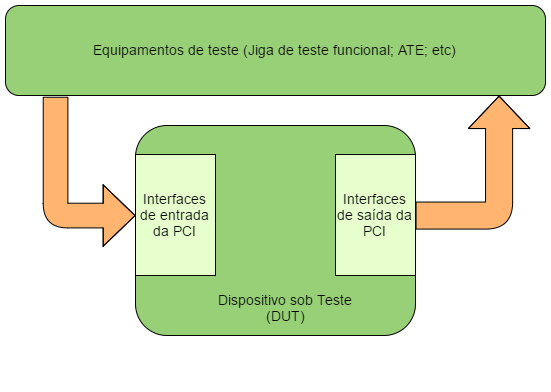
\includegraphics[width=0.8\linewidth]{fig/functionaltest}
            \caption{Diagrama de blocos de um esquema de teste funcional}
            \label{fig:funcblock}
\end{figure}

%geração de roteiros e estado da arte
A geração do roteiro de teste geralmente é manual e os esforços de pesquisa em teste funcional se concentram em métodos de automatização da geração de testes. O trabalho de \citet{thibeault2006} propõe uma investigação em otimização de roteiros e reuso de padrões de teste gerados diretamente por ferramentas de validação de projeto. 

Também existem trabalhos mais recentes de automatização de testes funcionais, como o de \citet{riefert2014effective}, que desenvolveu um método automatizado para testes funcionais em processadores utilizando métodos formais.


%Em \citep{thibeault2006} ve-se que que é importante considerar que, mesmo com suas vantagens, é crescentemente difícil justificar o uso de testes funcionais em velocidade nominal como abordagem principal. Sob esta perspectiva, parece que um teste funcional em velocidade nominal será mais e mais restrito à partes do DuT sem suporte à varredura periférica \citep{thibeault2006}. Todavia, a captura de defeitos relacionados à temporização não é o único aspecto positivo do teste funcional. Sua natureza não serial também pode ser explorada para propósitos de otimização de testes. Em [But100], foi proposto a criação de um pequeno conjunto de padrões de teste moderadamente rápidos, inseridos de inicio no programa de teste, de maneira a obter vantagem de sua inicial má capacidade de detecção de dispositivos enquanto mantem custos de desenvolvimento a um nível aceitável. Estas propostas foram baseadas no fato de qeu é mais difícil e caro criar e depurar padrões quando a frequência do  padrão funcional é perto da velocidade especificada do dispositivo.

\section{Padrões de projeto em LabVIEW}

Padrões de projeto são formas bem estabelecidas para resolver problemas comumente recorrentes. Não se trata de um código fonte ou \textit{framework}, mas de uma descrição de como se resolver um problema que pode ser aplicado em diversas situações. Padrões de projeto ganharam popularidade na ciência da computação após a obra de \citet{gamma1994design}. 

As vantagens de usá-los estão na facilidade dos desenvolvedores em reconhecê-los no código fonte, de dispensarem a necessidade de reinventar soluções para problemas recorrentes, como também na confiança de estar aplicando uma solução bem trabalhada para um tipo de problema.

No caso específico do LabVIEW, os padrões de projeto podem ser um modelo como um \textit{framework}, ou seja, uma base de códigos para o desenvolvimento da aplicação. Em \citet{blume2007labview} descrevem-se os principais padrões de projeto e \textit{frameworks} da linguagem: as máquinas de estado; os laços acionados por evento; o produtor-consumidor; o tratador de mensagem em fila; a máquina de estados em fila; e o Modelo de Atores.

\subsubsection{Máquinas de Estados Finitos}
As máquinas de estados finitos (figura \ref{fig:statemachine}) são amplamente conhecidas e, nelas, o comportamento dinâmico do programa depende de estados cujas transições dependem de uma lógica de estados. É fundamental a criação de uma tabela de estados para uma máquina de estados efetiva.

\begin{figure}
    \centering
        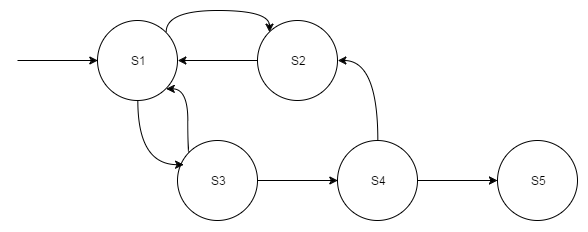
\includegraphics[width=0.8\linewidth]{fig/patt/statemachine}
            \caption{Um exemplo de máquina de estados finita}
            \label{fig:statemachine}
\end{figure}

\subsubsection{Laços Acionados por Eventos}
Nos laços acionados por eventos (figura \ref{fig:eventloop}), diferentemente do paradigma procedural, a execução do programa é decidida em tempo de execução: o programa permanece em estado de espera até a ocorrência de um evento e seu despacho para um tratador. Esta técnica poupa tempo de CPU e é uma boa alternativa ao uso de \textit{pooling}, além de poder ser aplicada em qualquer sistema de acionamento de processos escravos.

\begin{figure}[h]
    \centering
        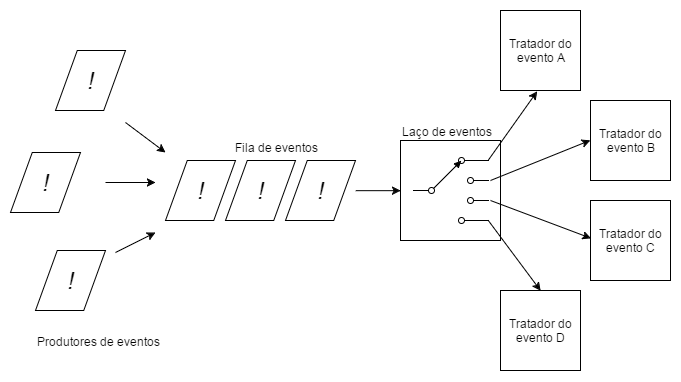
\includegraphics[width=1\linewidth]{fig/patt/eventloop}
            \caption{Laço acionado por eventos}
            \label{fig:eventloop}
\end{figure}

\subsubsection{O Produtor - Consumidor}
O produtor-consumidor (figura \ref{fig:prodcon}) é normalmente aplicado quando se precisa executar tarefas assíncronas e comunicar entre elas sem perda de desempenho, caso uma dependa da outra. Este padrão tem por característica a relação de mestre/escravo entre os laços e a independência no fluxo de dados entre eles. Uma tarefa produzindo dados ou comandos e uma ou mais tarefas consumindo o que a produtora gera. A comunicação entre as tarefas é realizada por filas, ou seja, os dados são enfileirados e desenfileirados em um \textit{buffer}, em esquema conhecido como \textit{first-in-first-out - FIFO}.

\begin{figure}
    \centering
        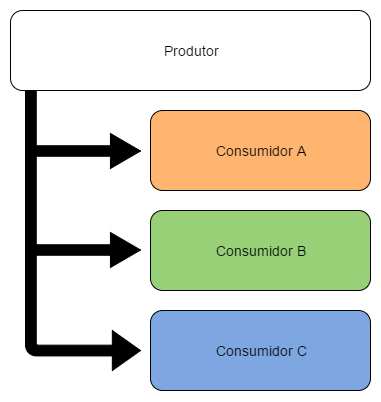
\includegraphics[width=0.5\linewidth]{fig/patt/produtorconsumidor}
            \caption{Diagrama do produtor-consumidor com 4 laços independentes comunicando por uma fila}
            \label{fig:prodcon}
\end{figure}

\begin{figure}
    \centering
        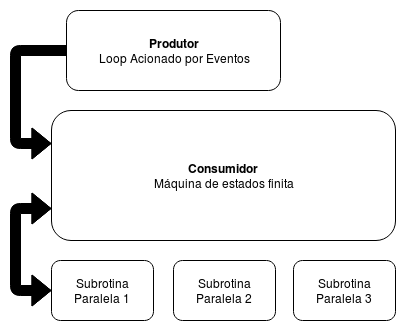
\includegraphics[width=0.7\linewidth]{fig/patt/tmf}
            \caption{Diagrama do tratador de mensagens em fila}
            \label{fig:tmf}
\end{figure}


\subsubsection{Tratador de mensagens em fila}
O tratador de mensagens em fila - TMF (figura \ref{fig:tmf}) ou, em inglês, \textit{Queue Message Handler} ou \textit{Queue-driven State Machine}, é uma extensão do produtor-consumidor, possibilitando que processos escravos possam atuar também como produtores e comunicar entre si. Normalmente apresenta-se como na figura \ref{fig:tmf}, com um laço mestre acionado por eventos criando tarefas, um processo principal e subprocessos auxiliares. O TMF não só é um padrão de projeto, mas também a arquitetura base de muitas aplicações de média a grande complexidade. É usado em aplicações que exijam interfaces de usuário responsivas, aplicações multitarefa e o desacoplamento de processos.


\subsection{Framework de Atores}
\label{actorframework}


%\subsubsection{A necessidade de um outro modelo de computação concorrente}

Na programação imperativa, assim como na maior parte dos paradigmas e linguagens de programação, as \textit{threads} são a solução tradicional para problemas de concorrência. Entretanto, programação concorrente baseada em \textit{threads}, \textit{locks} e estados compartilhados são ditas difíceis de fazer e propensas a erro \citep{Erb2012}. 

Em 1973, \citet{hewitt1973session} criou o modelo de atores como alternativa às \textit{threads} em problemas de computação concorrente e sistemas distribuídos. Sua premissa é a de que qualquer computação fisicamente possível pode ser diretamente implementada usando Atores \citep{hewitt2010actor}. 

 A abordagem no modelo de atores é totalmente diferente, já que retira inteiramente a noção de estado compartilhado. Ainda é possível que haja estados, entretanto, estes estão exclusivamente acoplados a uma única entidade, chamada Ator.

O modelo tem sido usado tanto como uma estrutura base para compreensão de problemas de concorrência, como também como base teórica para diversas implementações práticas de sistemas concorrentes. O crescimento de sistemas concorrentes massivos de computação em nuvem e processadores \textit{multi-cores} tem aumentado o interesse por este modelo. Exemplos de sistemas modelados pelo sistema de atores incluem: sistemas de email, Serviços Web e Objetos com \textit{locks}.

\subsubsection{Conceitos fundamentais do modelo}

Um ator é a unidade primitiva de computação. Ao receber uma mensagem, um ator pode concorrentemente \citep{hewitt2013computation}:

\begin{itemize}
    \item Criar um finito número finito de novos atores;
    \item Enviar finitas mensagens para outros atores;
    \item Designar como tratar a próxima mensagem que receber, alterando seu estado interno.
\end{itemize}

%Comunicação Assíncrona.
Para comunicação, o modelo de atores usa a troca de mensagens assíncronas, atribuindo a cada ator a sua caixa de mensagens (figura \ref{fig:actor}), local onde as mensagens são armazenadas enquanto o ator processa a mensagem anterior. Num sistema de atores, tudo o que um ator sabe do outro é o endereço de sua caixa de mensagens.

O ator sempre trabalha em resposta às mensagens que recebe, tratando-as sequencialmente, uma de cada vez \citep{Erb2012}. Isso significa que, para executar múltiplas mensagens de forma concorrente, será necessário que antes se crie um ator para cada uma delas. 

    \begin{figure}
        \centering
        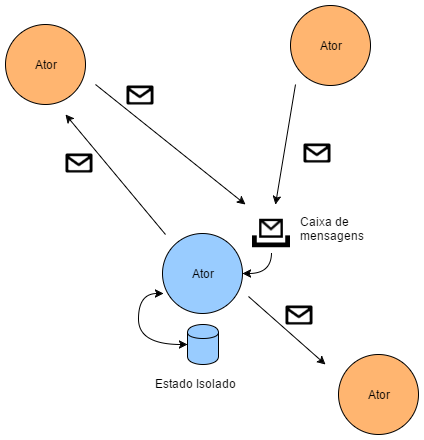
\includegraphics[width=0.9\linewidth]{fig/actor}
        \caption{Um exemplo de uma rede com alguns atores, com destaque para um ator, sua caixa de mensagens e seu estado interno. Adaptado de \citet{Erb2012}}
        \label{fig:actor}
    \end{figure}
 
O ponto central do modelo de atores, e o que o diferencia das \textit{threads}, é que não existe compartilhamento de memória ou estado, sendo completamente isolados uns dos outros. \citet{Erb2012} enfatiza que a implementação de estados privados é fundamental para um sistema no modelo de atores.

\subsubsection{Distribuição e Escalabilidade}

A natureza assíncrona e sem compartilhamento de estados do modelo de atores assemelha-se à comunicação em rede, o que permite a implementação de sistemas distribuídos. De fato, muitas das implementações do modelo de atores oferecem essa funcionalidade e possibilitam a fácil extensão do sistema para múltiplas máquinas em um sistema concorrente e distribuído \citep{hewitt2010actor, Erb2012}. 

Pela sua simplicidade e isolamento entre atores, o modelo permite o escalonamento de aplicações pelo instanciamento e replicação de atores e distribuição por outras máquinas.

\subsubsection{Robustez e tolerância a falhas em tempo de execução}

Sistemas concorrentes baseados em \textit{threads} dificilmente conseguem ter boas soluções de tolerância a faltas por causa do não-determinismo associado ao compartilhamento de estados e apreensão de recursos (\textit{locks}) \citep{Erb2012}. 

O modelo de atores normalmente adota uma política de \textit{deixar quebrar}. Isso porque a maneira isolada e de não compartilhar nada dos atores permite que um ator quebre sem influenciar os outros atores. Além do mais, pode-se usar atores em hierarquia para supervisionar possíveis falhas de atores \textit{filhos}, conforme visto em \citet{Erb2012}. Isso permite criar sistemas que se recuperem sozinhos, de forma que, se um ator do sistema quebrar, o sistema tem como detectar o problema e colocar o sistema em um estado consistente novamente. 

A política de deixar quebrar é enxuta, já que dispensa a necessidade de criar infinitos tratadores para muitos problemas, que talvez nunca ocorram, e a implementação de outras politicas de Programação Defensiva.

% Overly defensive programming however introduces unnecessary code for errors impossible to even happen, thus wasting runtime and maintenance costs. There is also the risk that the code traps or prevents too many exceptions, potentially resulting in unnoticed, incorrect results.https://en.wikipedia.org/wiki/Defensive_programming

\subsection{Implementação em LabVIEW}

O modelo de atores possui implementações em inúmeras linguagens, tanto no paradigma orientado a objetos, como também no paradigma funcional. Em LabVIEW, sua implementação foi realizada por meio de um \textit{framework}, ou seja, uma estrutura básica de programa na qual uma aplicação pode ser construída.

No texto de \citet{smithAF}, constata-se que esta implementação é mais restrita do que em outras linguagens. Primeiro que, no \textit{framework} de atores, a comunicação de um ator é limitada a mensagens para o ator que o criou, atores que ele criou ou para sí mesmo (ver figura \ref{fig:actormsg}). Essa hierarquia, por um lado, obriga a criar atores supervisórios, mas também restringe a comunicação entre a rede de atores.

A implementação dos atores não são estruturas leves e \textit{atômicas} como proposto por \citet{hewitt1973session}, mas objetos sobrecarregados por diversas camadas de sub-rotinas\footnote{Uma sub-rotina em LabVIEW é também referida como \textit{subVirtual Instrument} ou \textit{subVI}.}. Isto impede a construção e destruição irrestrita de atores. Todavia, o \textit{framework} ainda detém grande flexibilidade de arranjos de atores e hierarquias de programa.


\begin{figure}[h!]
    \centering
    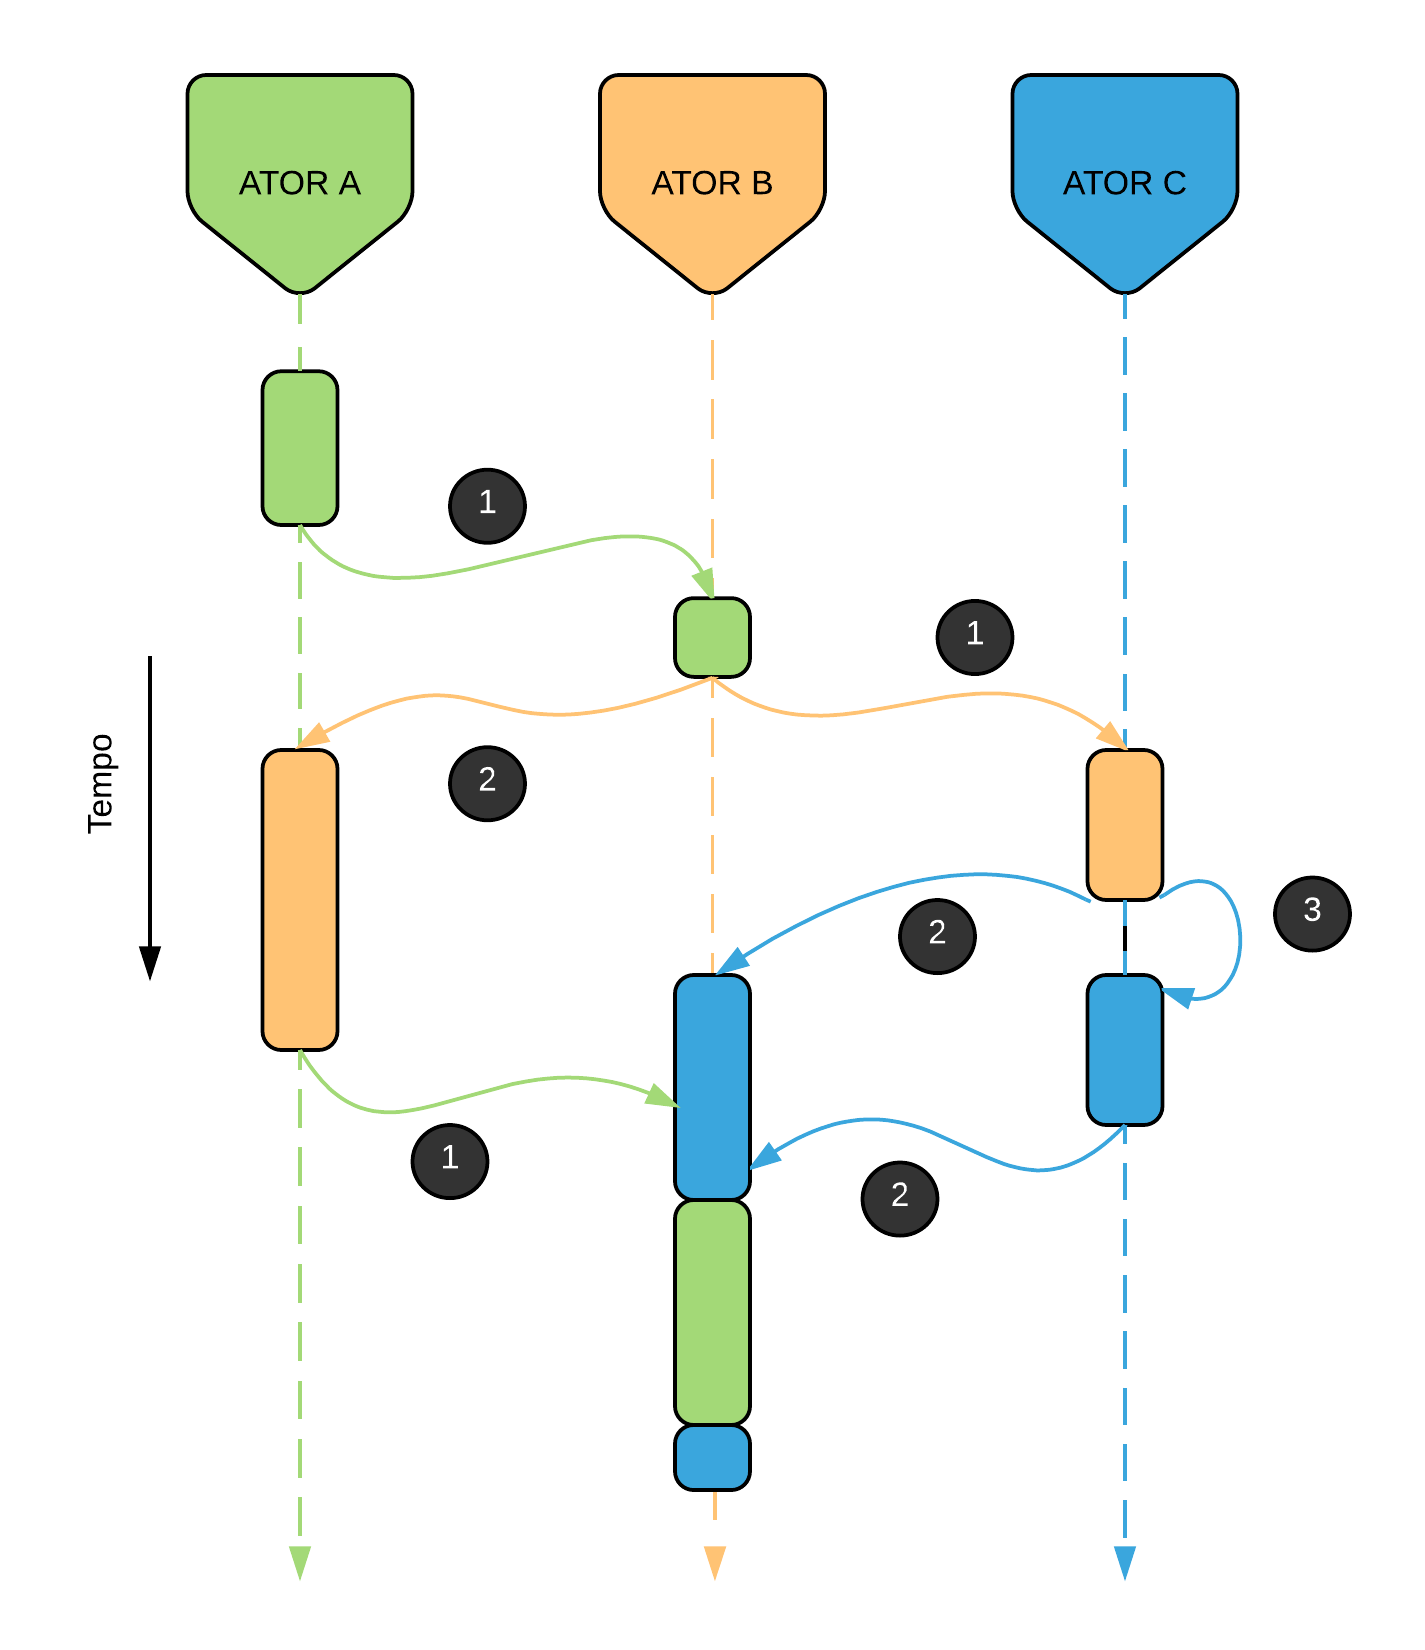
\includegraphics[width=0.9\linewidth]{fig/actormsg}
    \caption{Mensagens no \textit{framework} de atores em LabVIEW: (1) atores podem mandar mensagens para seus filhos; (2) atores podem mandar mensagem para os seus pais; (3) atores podem mandar mensagem para si mesmos}
    \label{fig:actormsg}
\end{figure}

Um ponto curioso do \textit{framework} é o suporte às mensagens síncronas entre atores \citep{smithAF}, funcionalidade que cria um compartilhamento de estado e rompe com a proposta do modelo.

% https://books.google.com.br/books?hl=en&lr=&id=s4AR6y1cp5EC&oi=fnd&pg=PA159&dq=actor+model&ots=x-POw6gaOc&sig=AhvfbolBXNsxexNgxGVpMoqShKs#v=onepage&q=actor%20model&f=false
% https://arxiv.org/ftp/arxiv/papers/1008/1008.1459.pdf
% http://berb.github.io/diploma-thesis/original/054_actors.html

\begin{comment}

O que eu quero falar na revisão?
Esta revisão bibliográfica pretende atingir dois objetivos: a revisão do estado da arte em teste de  placas eletrônicas, e também dos fundamentos do uso de programação concorrente, foco deste trabalho


Definir teste e diagnóstico.
Teste é o procedimento de checagem realizado para garantir a qualidade, desempenho, e confiabilidade de algo antes de ser colocado em uso
Diagnóstico é a identificação de uma causa raiz de um problema pela examinação de seus sintomas.
Metricas

O que eu quero falar na revisão?
Esta revisão bibliográfica pretende atingir dois objetivos: a revisão do estado da arte em placas eletrônicas, e também dos fundamentos do uso de programação concorrente, foco deste trabalho
\end{comment}
    \chapter{Especificação do programa}
\label{specs}
%\addcontentsline{toc}{chapter}{Estudo de caso}

% Definição/especificação do problema tratado
% limitações e o que foi escolhido resolver, tendo como conclusão que tipo de problema temos
% em metodologia isso vira uma solução

%Esta sessão descreve e delimita o escopo deste trabalho.

% O PROGRAMA ANTERIOR TERIA QUE IR PARA CONTEXTUALIZAÇÃO.
% Este trabalho é um port de um programa anterior, e vamos discutir o seu estado



% estado da arte avançado mas o dispositivo não acompanha


A partir do estado da arte em teste e diagnóstico estudado, nota-se que a configuração de teste de manufatura estudada pode ser aprimorado em diversos aspectos, principalmente em hardware. Entretanto, este trabalho se limita ao desenvolvimento de um novo programa de teste de manufatura e decidiu-se limitar o escopo do trabalho a um único produto e manter a mesma configuração de teste: bateria de testes, roteiro e a mesma jiga. No início deste capítulo são detalhados o objeto de teste, o acesso ao teste que ele suporta, a jiga e instrumentos de medição utilizados, enquanto o final se reserva para discutir as especificações de software.

\section{O dispositivo sob teste}

    O dispositivo sob teste é um módulo de telemetria para sistemas de infraestrutura de água e energia, mais especificamente para atender o setor de distribuição de energia. A funcionalidade principal do produto é o módulo M2M de comunicação móvel (High Speed Packet Access - HSPA) com interpretador Java™. Possui como funcionalidades secundárias: sensoriamento de tensões trifásicas, atualização remota de \textit{firmware}\footnote{\textit{Over-the-air provisioning} é um método remoto de atualização de software. Isso é normalmente implementado no próprio \textit{bootloader} do sistema \citep{jacobbeningo2013}.}, sistema de alimentação emergencial (bateria ou supercapacitor), portas digitais para detectar a abertura de gabinete, porta RS-232 para comunicação com religadores e outras funcionalidades que podem ser inseridos à pedido do cliente. Sua PCIM pode ser vista na figura \ref{fig:placa}. 
    
          
    \begin{figure}
        \centering
        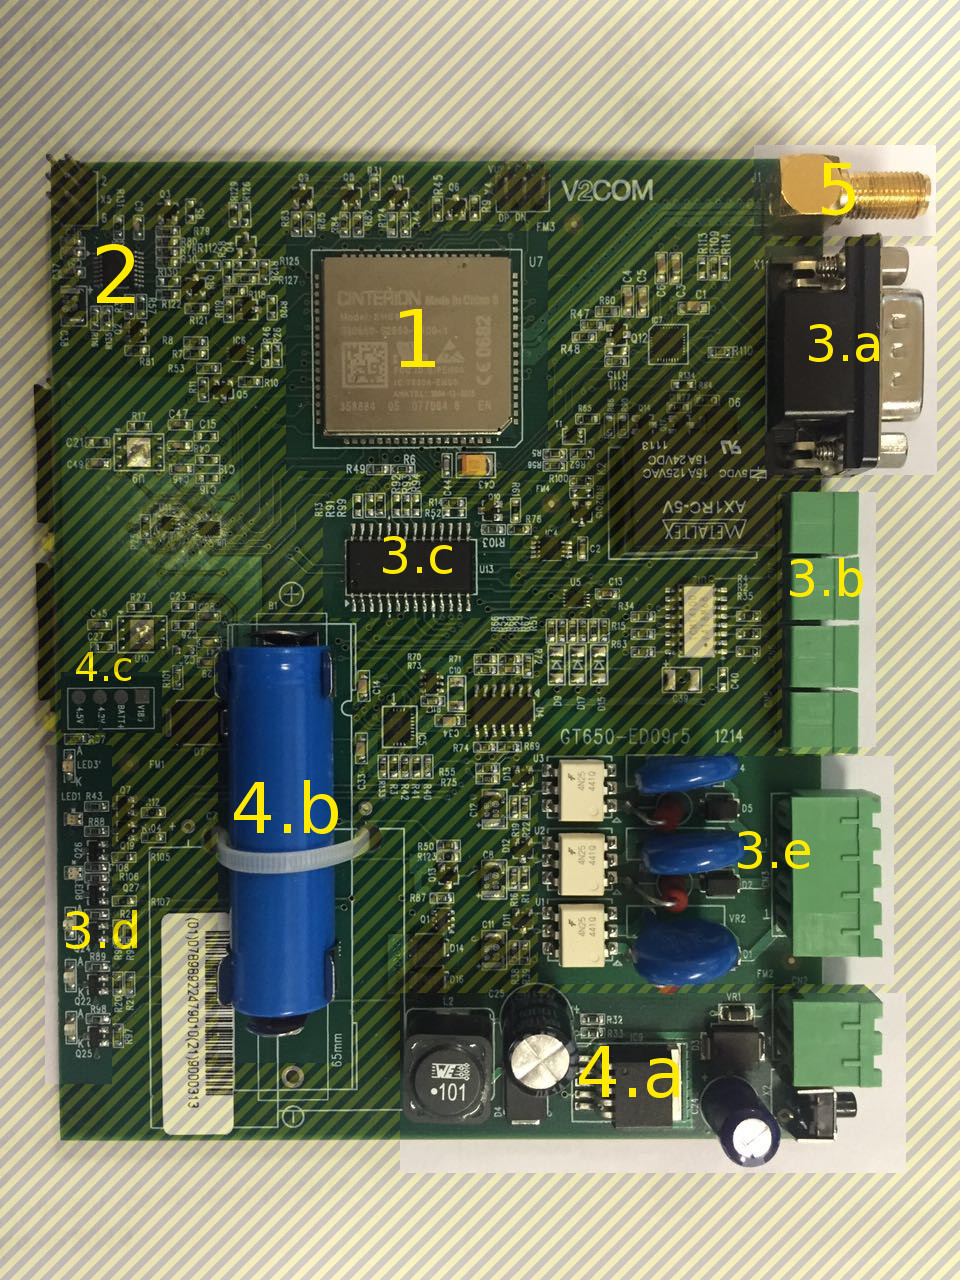
\includegraphics[width=0.92\linewidth]{placa}
        \caption{Foto do GT650 com destaque aos componentes da placa: o \textit{modem} EHS6 (1); o microcontrolador monitor \textit{watchdog} (2); o conector DB9 com duas portas RS232 (3.a); as E/S isoladas (3.b); o expansor de E/S por I$^{2}$C (3.c) ; o painel de LEDs indicativos (3.d); os detectores de tensão trifásica (3.e); o conversor buck (4.a); a bateria e o seu sistema de gerenciamento (4.b); os pontos de teste de alimentação (4.c); e o conector da antena (5) (foto do autor).}
        \label{fig:placa}
    \end{figure}
    
    \subsection{Módulo M2M}
        O \textit{modem} EHS6 da Cinterion (ponto 1 da figura \ref{fig:placa}) é o processador principal da placa, com comunicação TCP/IP via GSM/3GPP/GPRS, Intepretador Java e outros recursos comuns, como interface serial e I$^{2}$C. Segundo o \textit{datasheet} do fabricante \citep{cinterion2016}, o circuito integrado oferece: 
        %todo cite EHS6 DATASHEET
        
        \begin{itemize}
            \item Comunicação de dados 3G (HSPA): 800/850/900/1900/2100 MHz
            \item GPRS/EDGE Class 12: 850/900/1800/1900 MHz
            \item Suporte a Java™ ME\footnote{Java Micro Edition é  uma plataforma Java para sistemas embarcados} 3.2, com suporte a \textit{multithreading} e execução de múltiplas aplicações, além de 6 MB de memória RAM e 10 MB de memória Flash;  %todo cite JAVA ME
            \item Pilha de protocolos TCP/IP embarcada e acessível por comandos AT, incluindo conexão segura via TLS/SSL; serviços DNS e Ping; Cliente FTP e HTTP; %todo cite AT Commands
            \item Interface USB 2.0 HS e duas portas de interface modem serial;
            \item 16 GPIOs compartilhadas com as portas de comunicação, PWM e outras.
            \item ADC e interface I$^{2}$C; 
            \item Atualização de \textit{Firmware Over-the-air} (FOTA).
        \end{itemize}
        
        O fabricante não fornece informações internas sobre a arquitetura, como também nenhum meio de acesso à estrutura interna do módulo, como uma porta JTAG. Como contrapartida, a empresa oferece garantia de funcionamento, assim como suporte técnico completo. As consequências dessa política não são necessariamente positivas, conforme segue:
        
        Primeiro, impede a realização de testes estruturais e verificações mais profundas nos módulos, tanto na produção, quanto na manutenção, e torna todos os processos dependentes de agentes externos, de forma que o teste se limita à verificação de interconexões do \textit{modem} com seus periféricos, em um esquema similar aos testes centralizados por processador, vistos em \ref{FCT}. Outra dificuldade do EHS6 é seu encapsulamento LGA, que impede a completa verificação de solda por inspeção visual. Isso pode ser contornado, caso a empresa responsável pela montagem possua equipamentos de inspeção radiográfica.
        
        Segundo, que para todo e qualquer problema físico ou de \textit{firmware} que ocorrer com estes módulos, é necessário o envio ao fabricante original para solução, muitas vezes dependendo do suporte deste fornecedor em outro país. Por um lado, isto retira da empresa solicitante a responsabilidade de resolver problemas de baixo nível, assim como a necessidade de manter pessoal e equipamento especializado para analisar este tipo de falha. Por outro lado, trabalhar com componente e \textit{firmware} fechados deixa a produção sujeita a problemas invisíveis e cria uma situação de dependência com o OEM.
        
        Por estas limitações no teste estrutural, o escopo de teste elaborado é restrito às verificações funcionais administradas pelo próprio produto. 
        
    \subsection{Monitor \textit{Watchdog}}
    
        O MC9S08QG8 é um microcontrolador simples de 8 bits (figura \ref{fig:placa}, no ponto 2) e é  responsável por desligar o \textit{modem} por duas maneiras: a primeira pelo temporizador \textit{watchdog} e a segunda, pelo botão liga-desliga. 
        
        Também é armazenado nele o número de série da placa. Dessa forma, a empresa consegue separar o rastreamento dos \textit{modems} e das \emph{placas}, podendo intercambiá-las conforme necessário.
        
        Por estar conectado ao EHS6 como escravo I$^{2}$C, este componente é acessado e testado pelo mesmo. No teste funcional são realizadas as seguintes rotinas: captura do número de série, teste do botão liga-desliga e teste do temporizador \textit{watchdog}.
        
    \subsection{Interfaces de usuário e interconexões externas}
        Por ser uma solução de comunicação para outros equipamentos, o GT650 não possui interfaces digitais e analógicas muito complexas, exceto pela comunicação de dados via GSM, que será descrita à parte. Como pode ser visto na figura \ref{fig:placa}, a placa possui:
        
        \begin{itemize}
            \item Duas portas RS232\footnote{Uma é usada para comunicação por comandos AT e a outra para acessar os periféricos na porta I$^{2}$C};
            \item Três portas de entrada digitais opto isoladas; 
            \item Um relé de saída;
            \item Seis LEDs de sinalização;
            \item Uma porta para conferência de tensão trifásica.
        \end{itemize}
        
        Vale mencionar que as entradas e saídas digitais, assim como os LEDs, são controlados pelo \textit{modem} através do expansor de GPIO por endereçamento I$^{2}$C. Assim como no caso do microcontrolador de \textit{watchdog}, as verificações funcionais são acionadas pelo EHS6.

    \subsection{Conector e transmissor de radiofrequência (RF)}            
        
        O módulo não possui antena integrada e possui um conector SMA para a conexão de antenas externas. Neste caso, testa-se a potência do transmissor de radiofrequência através de um instrumento específico mencionado na seção \ref{instruni}.
            
    \subsection{Alimentação, bateria e BMS}
        O sistema de alimentação consiste em um conversor CC-CC de 12 Volts com saídas de 3,3 V e 5 V (figura \ref{fig:placa}-4.a) e uma bateria de lítio de 4,8 V, em caso de faltas na rede (figura \ref{fig:placa}-4.b). 
        
        Para testar este sistema, foram separados quatro pontos de teste na placa, como visto no ponto 4.c da figura \ref{fig:placa}: 5V, BATT+, 3V3, e 1.8V. Atualmente, o teste é realizado manualmente com o multímetro, ponto por ponto, mas enviando os dados de leitura pelas portas seriais do computador. 
                
\section{Cobertura e roteiro de teste}
        
    O roteiro de teste consiste numa verificação predominantemente funcional da placa do produto. Por não possuir um volume de produção que justifique a aquisição de um ICT, não possuir suporte ao IEEE 1149.1, como também por não conter nenhuma lógica programável no produto, o teste estrutural se limita às verificações realizadas na empresa de montagem, por verificações de solda e interconexões por AOI ou AXI. 
        
    Essa estratégia predominantemente funcional consegue atingir um bom controle de qualidade dos lotes, mas fracassa no diagnóstico de falhas e detecção de causas raiz. 

    A bateria de testes do produto é representada pelo fluxograma da figura \ref{fig:flowchart}. Nota-se que este roteiro é, em sua totalidade, sequencial, sendo o teste funcional das bandejas do cartão SIM a única etapa executada de forma concorrente. 
    
    \begin{figure}[h]
        \centering
        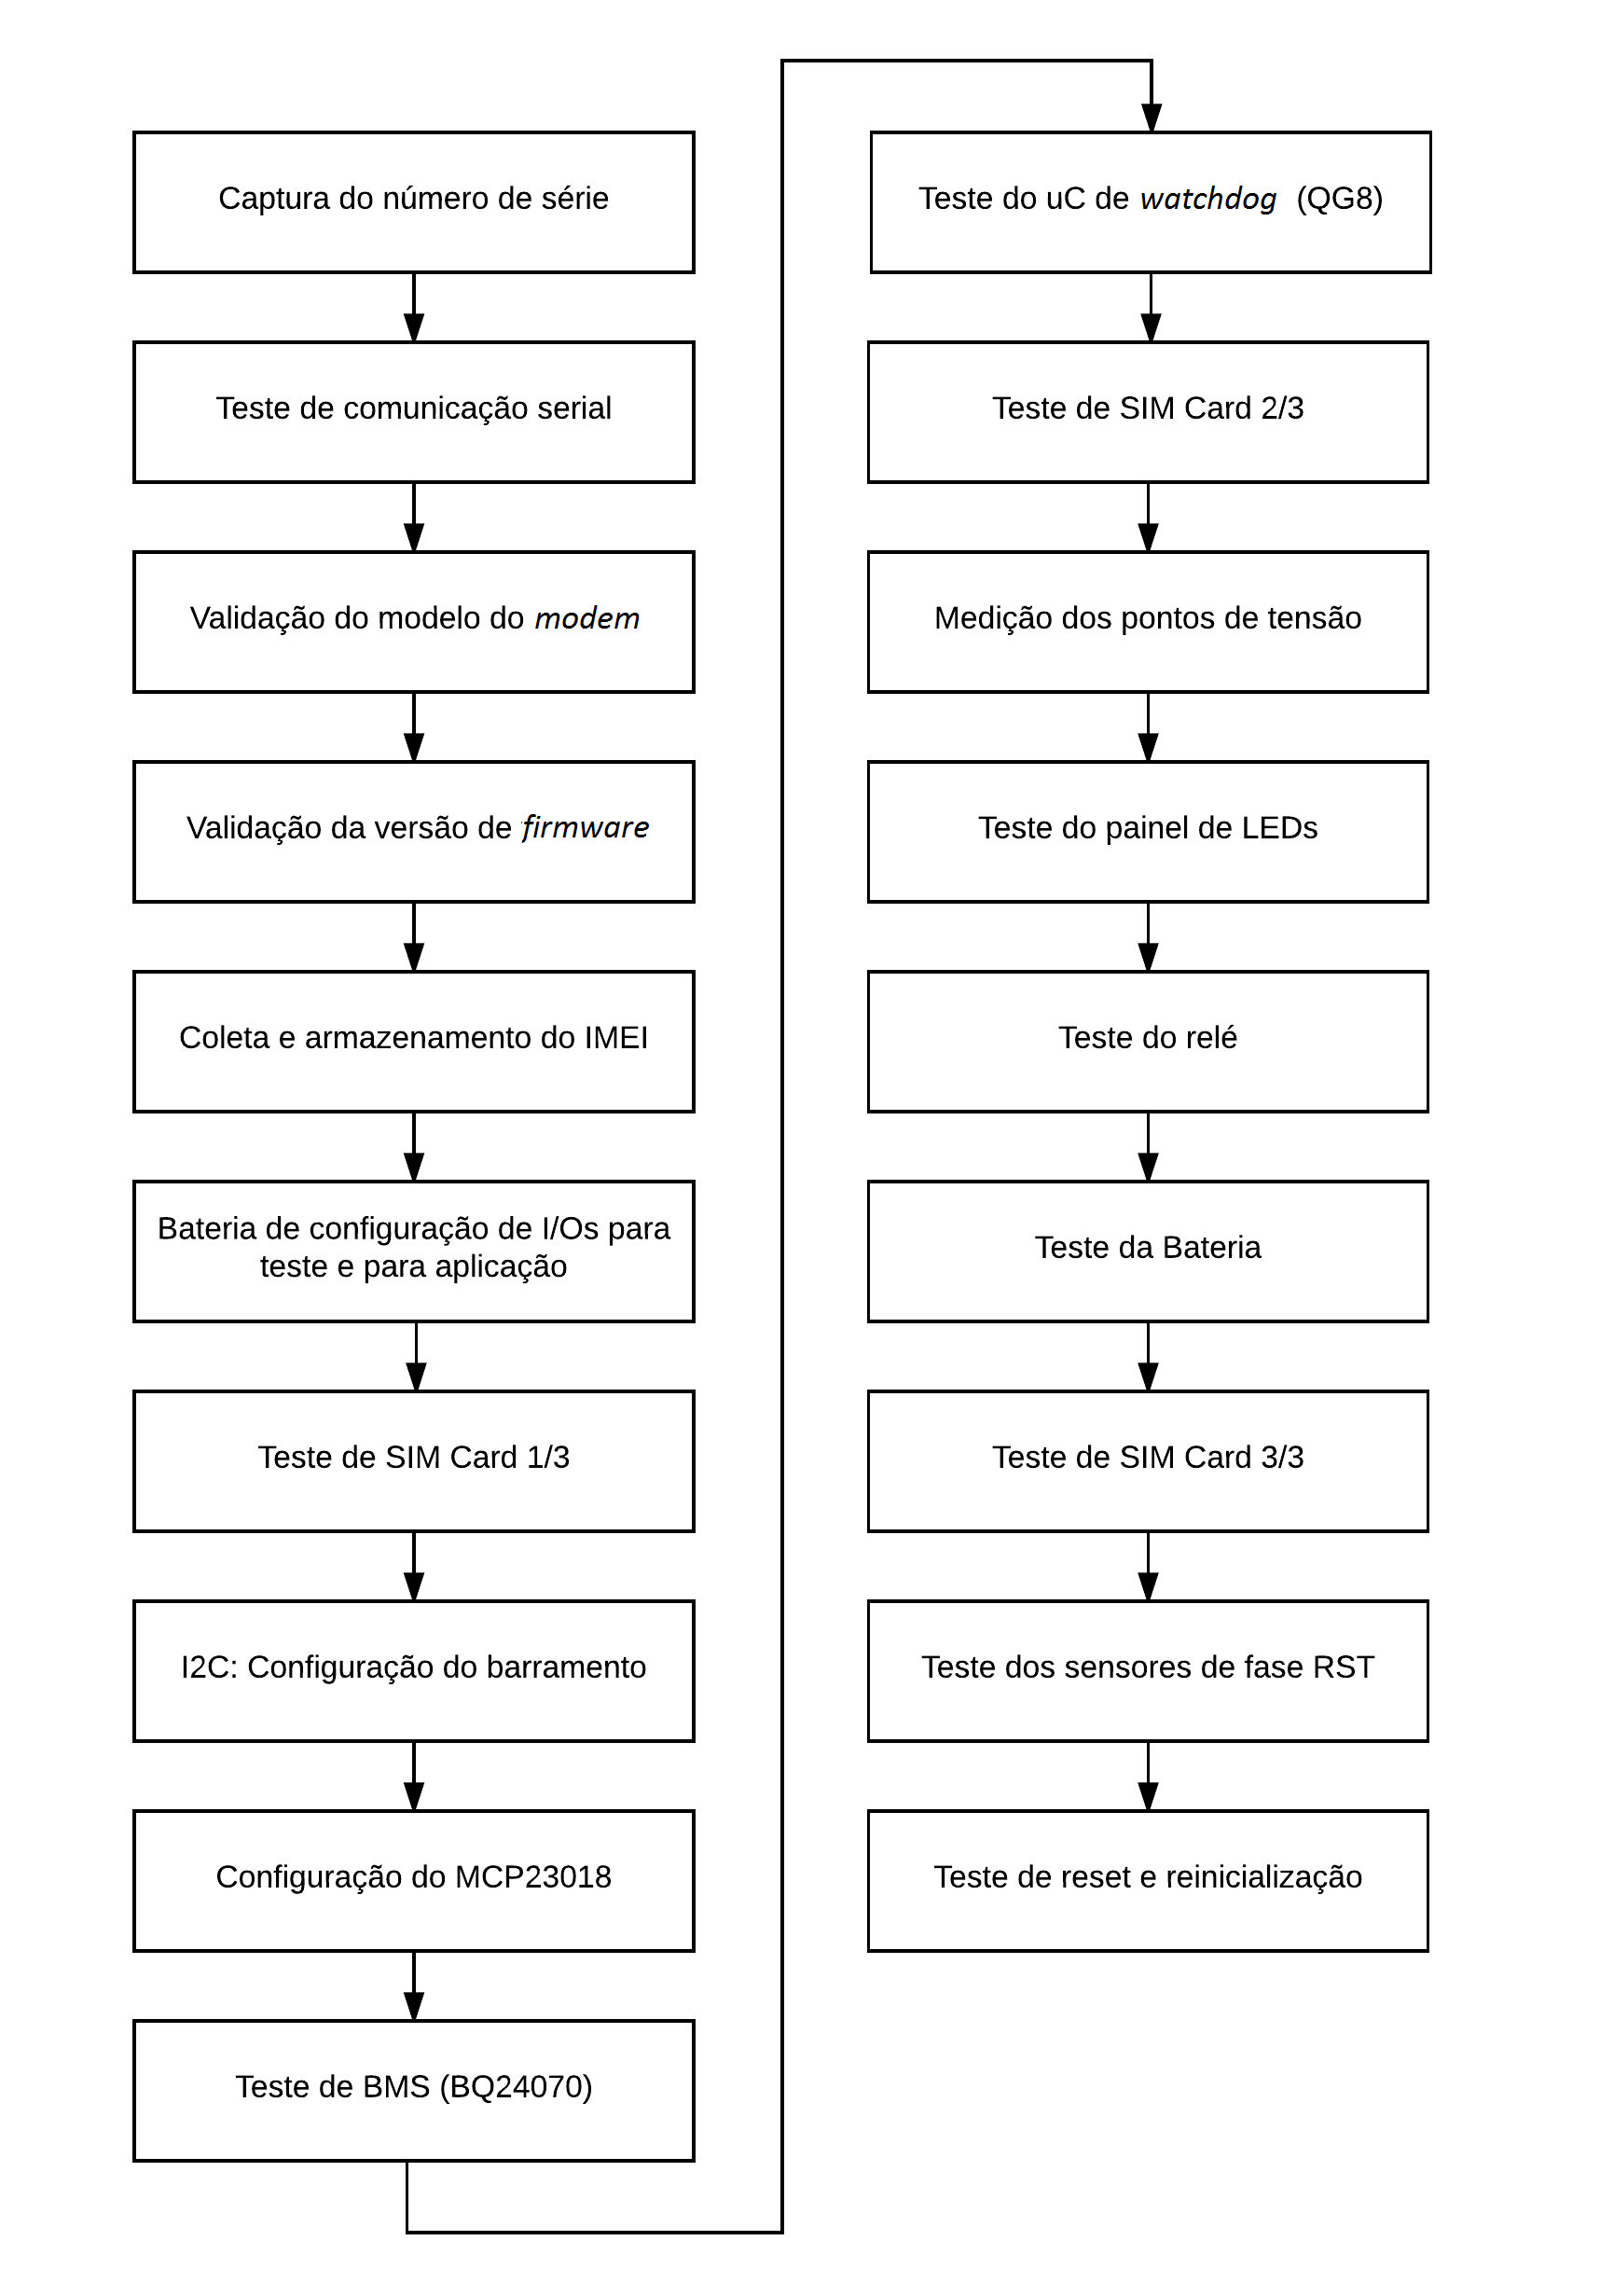
\includegraphics[width=0.9\textwidth]{model/fluxograma}
        \caption{Fluxograma da bateria de testes}
        \label{fig:flowchart}
    \end{figure} 
   
\section{A Jiga e os instrumentos de teste}
        
    A jiga utilizada foi desenvolvida para o teste funcional e provê interconexão para as interfaces externas do produto, exceto para o transmissor de radiofrequência. Fornece botões de interface para o operador controlar estímulos simples de sinais lógicos nas entradas e emular tensões trifásicas na porta respectiva. Ela também oferece um ponto de conexão do terra da placa para utilização do multímetro digital.
    
    \subsection{Multímetro}
        
        O multímetro utilizado é um ICEL MD-6400, com suporte de comunicação por uma porta serial RS232. A figura \ref{fig:dmmprotocol} exibe o protocolo que, a cada 250 ms, envia pacotes de 14 bytes de dados a uma \textit{baudrate} de 9600. 
          \begin{figure}[ht]
                \centering
                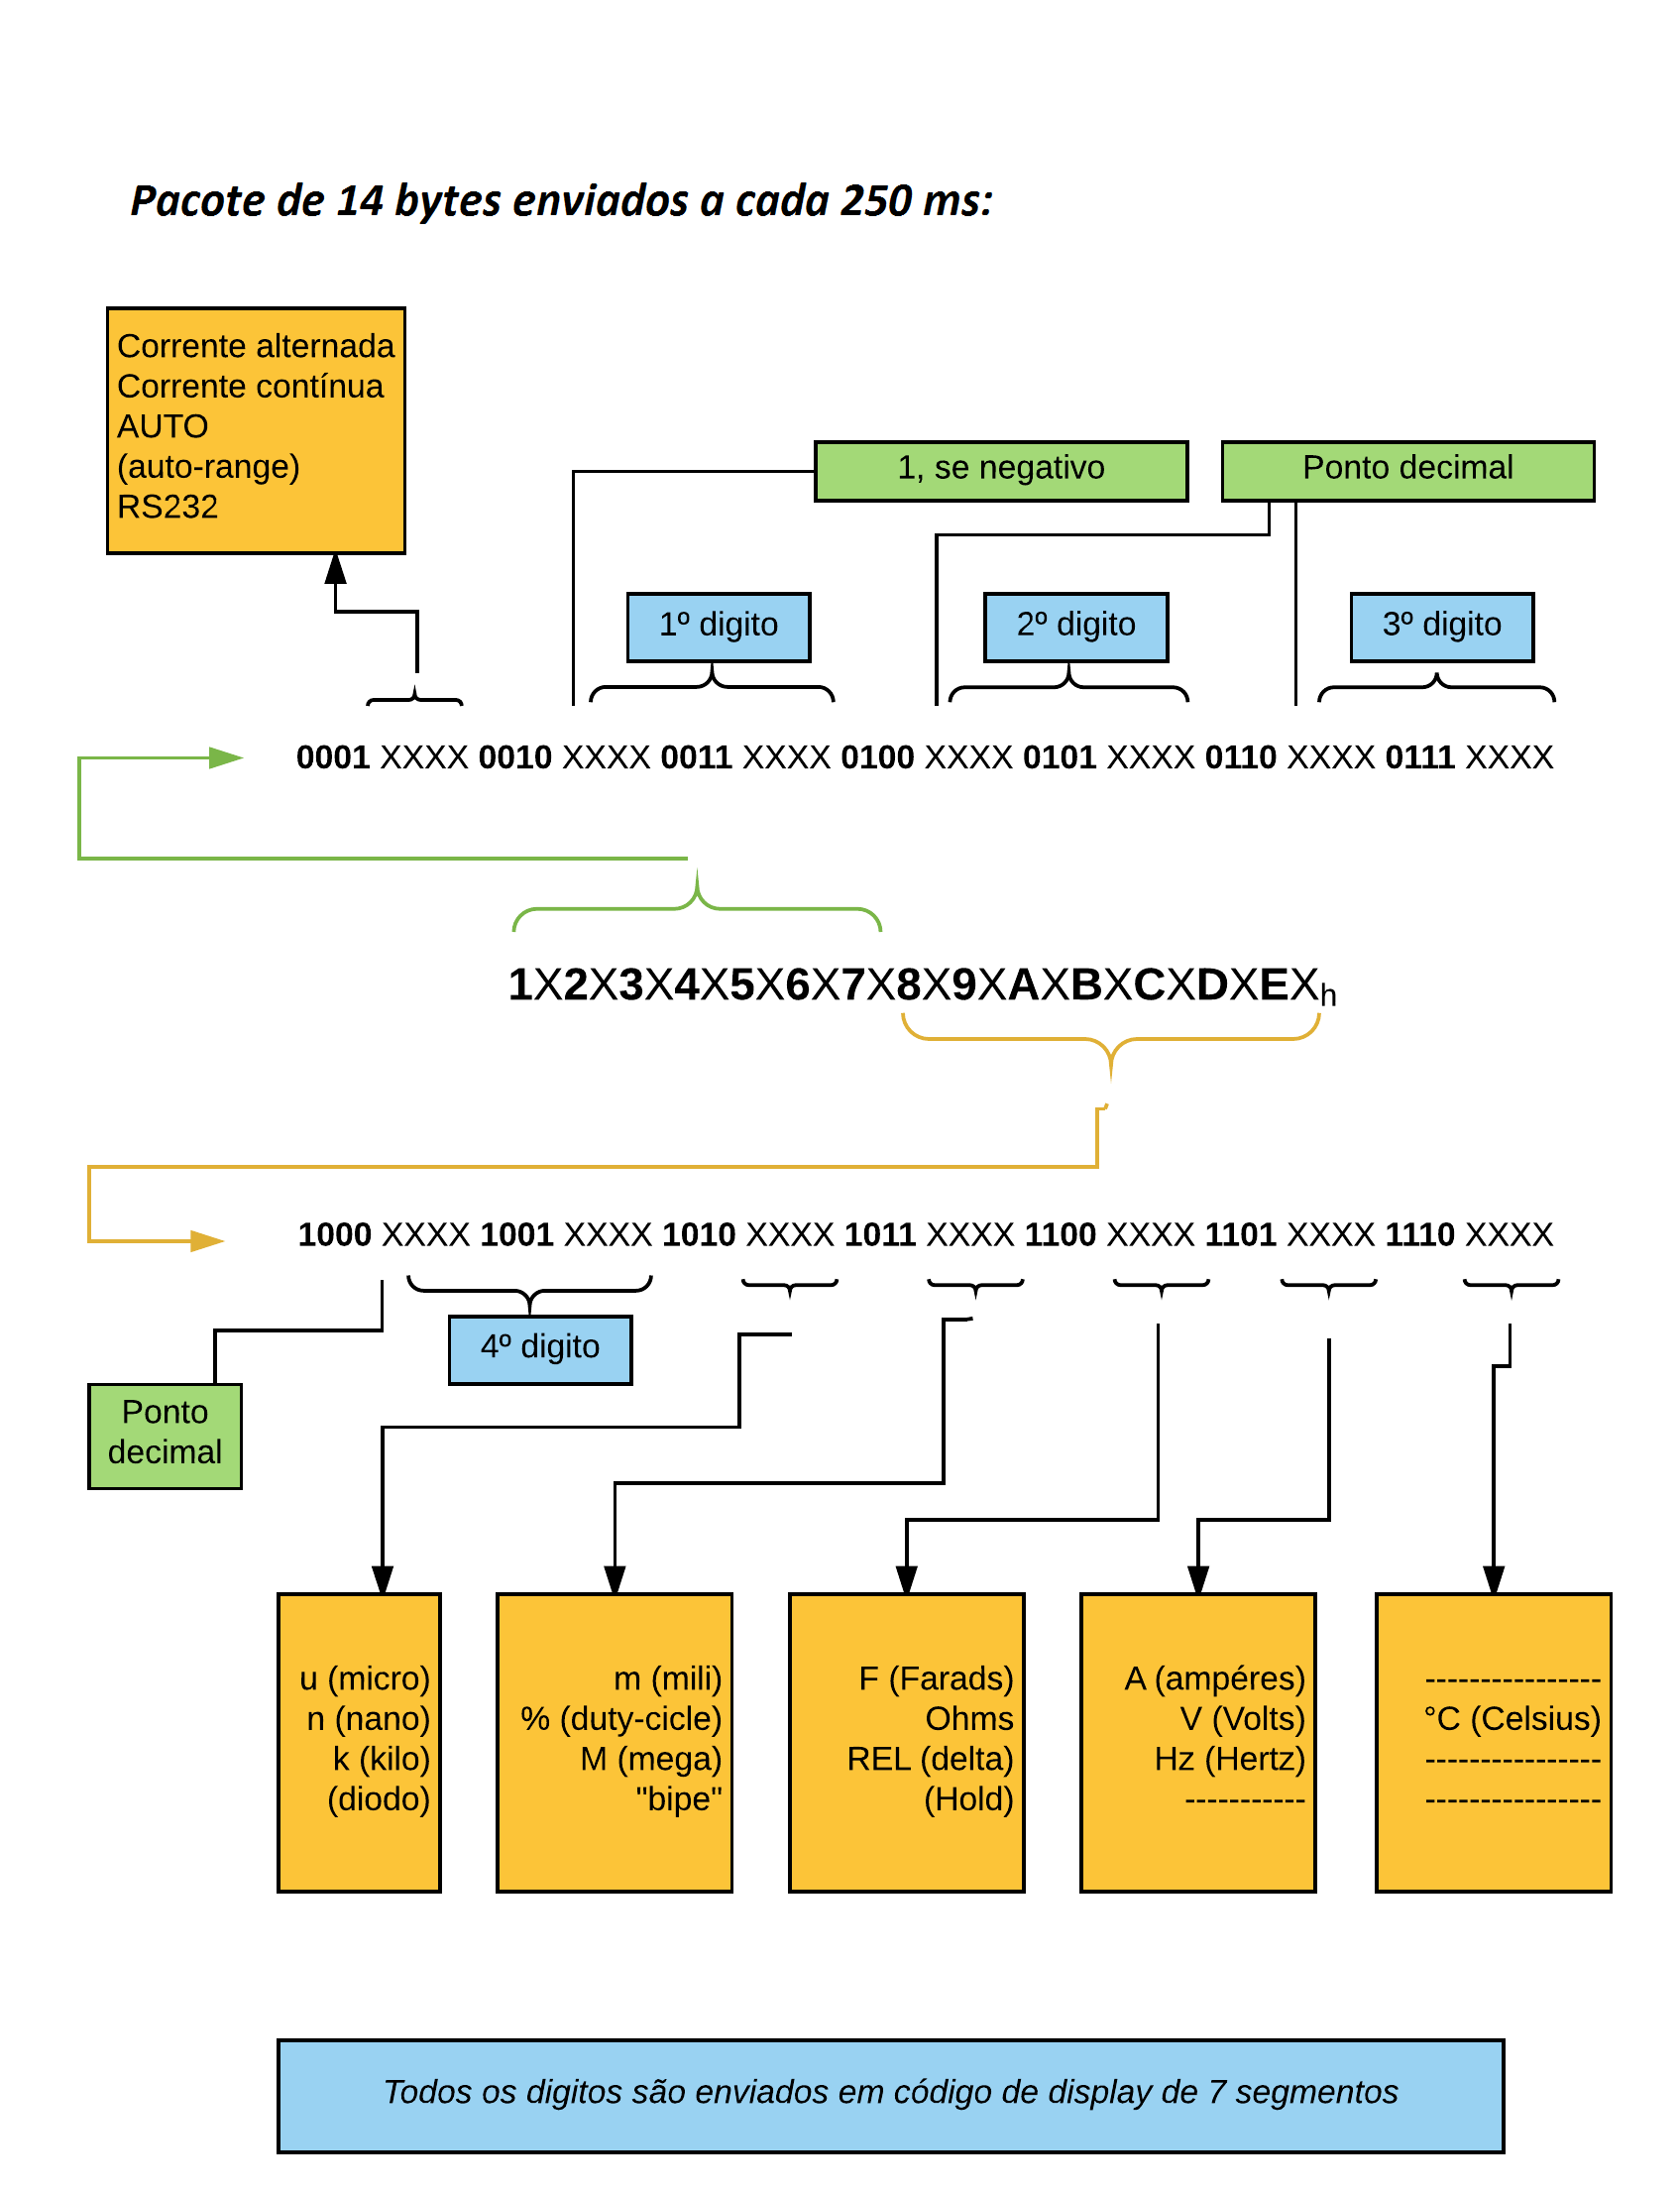
\includegraphics[width=\textwidth]{model/dmmprotocol}
                \caption{Estrutura de pacote de comunicação do multímetro}
                \label{fig:dmmprotocol}
            \end{figure}
    
    \subsection{Medidor de potência do transmissor}
    \label{instruni}
    % falar do programa de teste de potencia realizado anteriormente?
        O instrumento de medição de potência RF utilizado foi o NI 5680, da National Instruments, que mede potência RMS de sinais até 6 GHz, em larguras de banda bem estreitas (10-100 Hz de banda), e um limites de potência de entrada de -40 dBm a +23 dBm.

        \begin{figure}
            \centering
            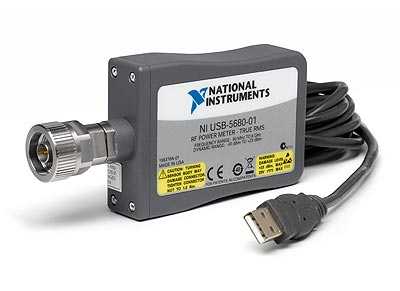
\includegraphics[width=0.7\textwidth]{usb5680.jpg}
            \caption{NI 5680 - instrumento utilizado para medição de potência RF}
            \label{fig:ni5680}
        \end{figure}
    
        % inserir http://sine.ni.com/nips/cds/view/p/lang/pt/nid/204499
        % datasheet http://www.ni.com/pdf/products/us/CAT_USB5680.pdf
        
        %falar como a bateria de medidas foi elaborada e a qualidade    delas
        
        % Atualmente é usado um medidor de potência RF -- O \emph{NI USB-5680} -- que tem uma faixa de frequência 50 MHz até 6 GHz, alcance de potência de -40 a +23 dBm, e uma banda de canal 10 a 100 MHz. Esta nova estratégia adotada, praticamente eliminou os retornos de campo por problemas de alcance do produto.
    
\section{Requisitos de Software}

        Requisitos de software são objetivos ou restrições estabelecidos pelos usuários e são divididos em requisitos funcionais e não funcionais \citep{bourque2014guide}.
        
        Requisitos funcionais definem as funcionalidades específicas que o programa deve oferecer, não necessariamente tratando das interações com o usuário, mas também como funcionalidades ocultas como, por exemplo, uma API ou interações com hardware.
        
        Requisitos não-funcionais são qualidades gerais de um programa como custo, usabilidade, modularidade e vários outros. Normalmente são requisitos difíceis de validar por sua natureza qualitativa. 
        
        A partir do contexto apresentado, foram levantados os seguintes requisitos não-funcionais do software:
        \begin{itemize}
            \item O programa deverá ser implementado em LabVIEW;
            \item Modularidade do programa e reusabilidade de código;
            \item Permitir o uso de concorrência e paralelismo na bateria de testes;
            \item Escalabilidade e flexibilidade de software para acompanhar alterações de hardware e da jiga de teste;
            \item Interface de usuário ergonômica e intuitiva.
        \end{itemize}
        
        Já os requisitos funcionais de software acompanham o que é testado pelo roteiro de testes anterior a este trabalho:
        \begin{itemize}
            \item Leitura e armazenamento do número de série colado na placa por um leitor de código de barras;
            \item Comunicação com o DUT via serial;
            \item Teste de comunicação das duas portas seriais;
            \item Verificação do modelo de \textit{modem};
            \item Verificação da versão da \textit{firmware} do \textit{modem};
            \item Armazenamento o IMEI\footnote{\textit{International Mobile Station Equipment Identity} ou Identificação Internacional de Equipamento Móvel é um número de identificação global e único para cada telefone ou \textit{modem} celular.} do \textit{modem};
            \item Configuração das GPIOs do \textit{modem} conforme o perfil da aplicação;
            \item Abertura, seleção e teste das duas bandejas de cartão SIM\footnote{\textit{Subscriber Identity Module}};
            \item Configuração e teste de comunicação $I^{2}C$;
            \item Configuração da operação do expansor de IO, MCP23018: interrupção espelhada, não incremento de ponteiro, interrupção push-pull;
            \item Configuração e teste do BQ24070, carregador de bateria e gerenciador de energia do sistema;
            \item Teste de leitura da bateria;
            \item Teste do MC9S08QG8, microcontrolador \textit{watchdog} e teste do botão liga e desliga;
            \item Leitura do número de série armazenado no MC9S08QG8, e validação deste com o número de série colado na placa;
            \item Teste de comunicação e leitura do sensor de temperatura LM75;
            \item Teste de finalização da sessão do terminal na porta serial ;
            \item Testes dos barramentos de tensão da placa: 4,5V, 4,2V, BATT++ e 1,8V;
            \item Teste do painel de LEDs;
            \item Teste de detecção de retirada e inserção da fonte de alimentação;
            \item Teste das 3 portas digitais;
            \item Teste de acionamento e desarme de relé;
            \item Teste da porta de tensão trifásica - detecção de presença e ausência;
            \item Teste de interrupção de desligamento e reinicialização do sistema;
            \item Teste de potência de sinal do transmissor de radiofrequência;
            \item Registro de execução de teste em arquivo de texto e resumo de teste em formato estruturado;
            \item Cliente WEB para envio automático à base de dados de produtos;
            \item Notificação para o operador sobre sucesso ou falha do teste, assim como possibilidade de reteste.
        \end{itemize}
    
    
    %Registro em servidor

    %A segunda classe de registro é um resumo estruturado da bateria de testes, o diagnóstico geral da placa e outras informações importantes para o controle e rastreamento dos produtos, requisito necessário para otimizações do processo produtivo como também do próprio produto.

\begin{comment}
    \subsection{Workflow do projeto} % jeitinho de trabalhar
       
     
     %   \subsection{Síntese dos requisitos ambientais de teste}
    % #todo
    
    Validação do projeto
    Controle de Qualidade
    Melhorias de processos
    Melhorias no produto
    Auxilio na Manutenção
\end{comment}    
    \chapter{Metodologia}
\label{metodologia}
%\addcontentsline{toc}{chapter}{Metodologia}

%  entendemos o contexto do problema, levantamos requisitos, agora vamos modelar e tentar aplciar padro~eos de projeto pra facilitar

% o que de técnica escolheu e da de usar
%o problema proposto era a criação de um progrmaa de teste concorrente em labview para o teste funcional da placa.
  
Ao considerar os requisitos de escalabilidade, concorrência, paralelismo e modularidade, nota-se que dentre os padrões de projeto revisados, o \textit{framework} de atores é o que melhor se ajusta como base para o programa, principalmente porque permite a criação de componentes isolados, naturalmente concorrentes e aplicáveis em diversas configurações de software e hardware. Além disso, é uma estrutura escalável, tanto na criação de mais atores na mesma máquina, como também para sistemas distribuídos.

Para a elaboração do modelo do sistema, utilizou-se de técnicas em Linguagem de Modelagem Unificada (do inglês \textit{Unified Modeling Language - UML)} para a sua representação e documentação \citep{rumbaugh2004unified}. Na etapa de implementação dos atores foram utilizados diversos padrões de projeto: máquinas de estado, tratadores de eventos, produtor-consumidores, e outros.

\section{Material Utilizado}
    \begin{itemize}
        \item Computador com uma instalação LabVIEW e com 3 portas RS-232;
        \item Multímetro ICEL MD-6400; 
        \item Um NI 5680 (\textit{powermeter} USB);
        \item Um GT650 e uma jiga de teste;
        \item Bibliotecas do Labview do modelo de atores, de comunicação serial e driver do \textit{powermeter}.
    \end{itemize}

    \chapter{Modelo e Implementação}
\label{modelagem}

    \section{Modelo do sistema no \textit{framework} de atores}
        
        %modelo do programa para o teste com a jiga anterior mas flexivel para expansao
        % partimos do pressuposto da flexibilidade no setup de teste, para depois adequar ao setup atual.
        
        Foram determinados cinco módulos, conforme as competências de teste necessárias: comunicação com o módulo; leitura e validação do multímetro; teste de potência de RF; registro da execução de testes; e supervisão; Para cada um destes módulos, foi criada uma classe de ator. 
        
        Dessa forma, permitem-se diversos arranjos de software e flexibilidade de adaptação frente à configuração física de teste utilizada. Para o caso da configuração de teste atualmente utilizada e selecionada para este trabalho, foi elaborado um arranjo em topologia em estrela, conforme visto na figura \ref{fig:modelo}. A escolha desta topologia foi consequente às próprias limitações do \textit{Actor Framework} em termos de comunicação entre atores, que não permite a comunicação de atores que não sejam \textit{pais} ou \textit{filhos}. A principal vantagem desta topologia é o Controlador como entidade supervisora natural do sistema, para detecção e tratamento de atores em falha de execução.
        
        \begin{figure}
            \centering
            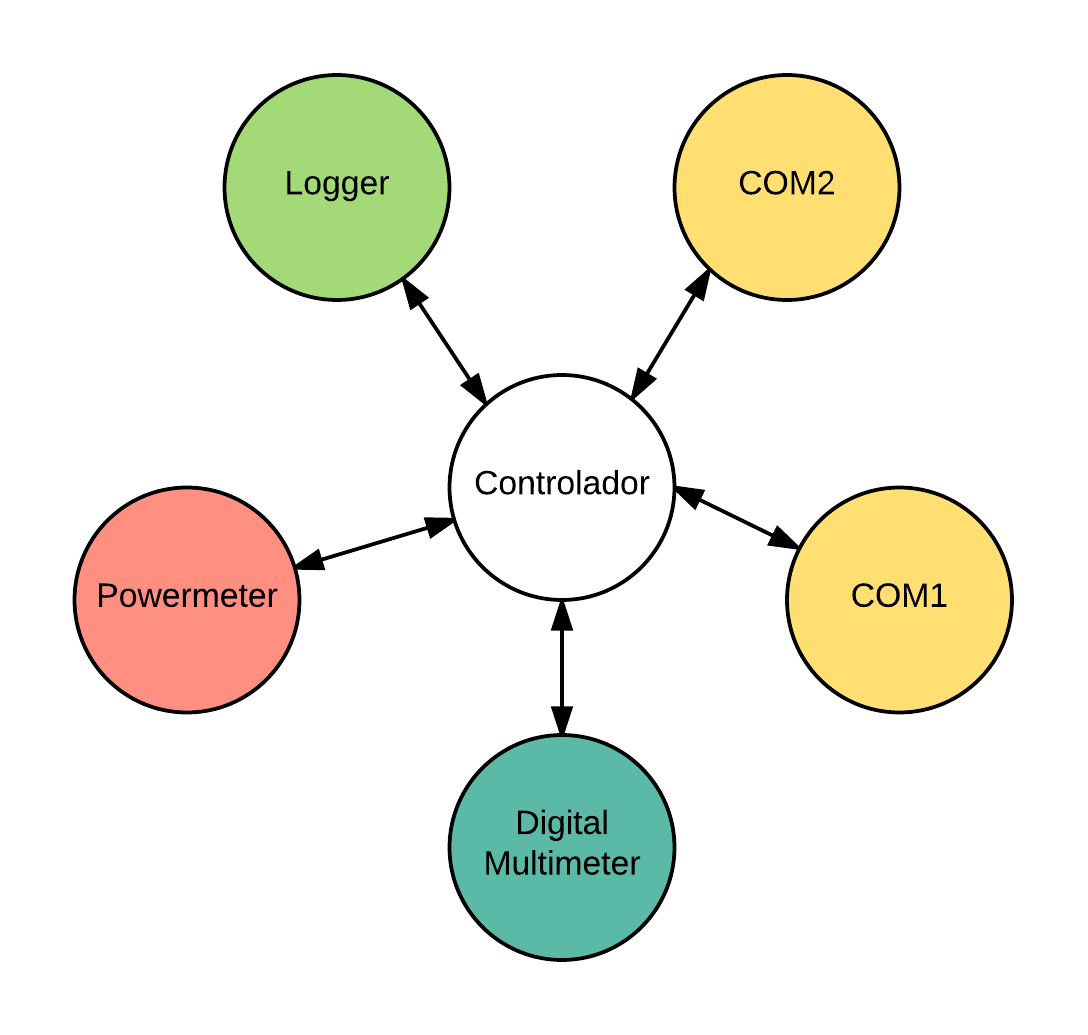
\includegraphics[width=0.9\linewidth]{fig/sistemmodel}
            \caption{Modelo do programa de teste reimplementado à partir do \textit{framework} de atores, e adequado para a jiga de teste legada}
            \label{fig:modelo}
        \end{figure}
            
        O Ator \texttt{ModCOM} é responsável pela comunicação com o DUT através de uma porta RS-232. Cumpre funções como enviar comandos de teste e verificar as respostas recebidas do dispositivo sob teste. Idealmente, este ator interpretaria trechos do roteiro da bateria de testes (em um arquivo xml), retornando o status da execução para o controlador. Todavia, devido ao curto prazo e simplificação do protótipo, a função de interpretação de roteiro foi deixada de lado. Dessa forma, o roteiro foi codificado diretamente no código fonte do programa, impossibilitando alterações de roteiro após a compilação.
        
        O ator \texttt{DMM} é incumbido pela leitura de dados do multímetro através da porta RS-232. A leitura dos pacotes do instrumento (figura \ref{fig:dmmprotocol}), sincronização e conversão de dados é realizada por ele, como também a interface de usuário para o operador do multímetro e a validação de medidas comparadas com a tabela de referências. 
        
        O registrador, ou \texttt{Logger}, é o ator responsável pelo registro da execução e resultados das baterias de testes. Dentre as suas incumbências estão: gerar um arquivo de registro completo do teste para fins de depuração e diagnóstico; gerar um arquivo de registro resumido para o controle de qualidade da produção e o envio direto dos registros para a base de dados de produção. 
                
        O Ator \texttt{Powermeter} detém o controle do medidor de potência RF, também referenciado como \textit{Powermeter}, responsável por toda a interface e configuração, e coleta de medições do NI 5680.
         
        O \texttt{Controller} ou controlador, como o próprio nome define, detém a responsabilidade sobre o fluxo de execução do programa, criando e destruindo os outros atores-módulos e fazendo a comunicação entre seus atores filhos. Além disso, detém a interface de usuário principal do programa.
        
        A relação entre as classes criadas com as classes base do \textit{framework} podem ser vistas no diagrama de classes UML da figura \ref{fig:classdiagram}. Nota-se que as mensagens entre atores possuem uma superclasse em comum e que, para cada ator, existem diversas classes de mensagens associadas a ele. Cada classe de mensagem se relaciona com um método interno do ator, funcionando como a interface pública deste ator. 
        Para melhor legibilidade, neste diagrama foram suprimidas as classes de mensagens, assim como muitas das VIs (\textit{Virtual Instruments}) das classes criadas.
        
            \begin{figure}
                \centering
                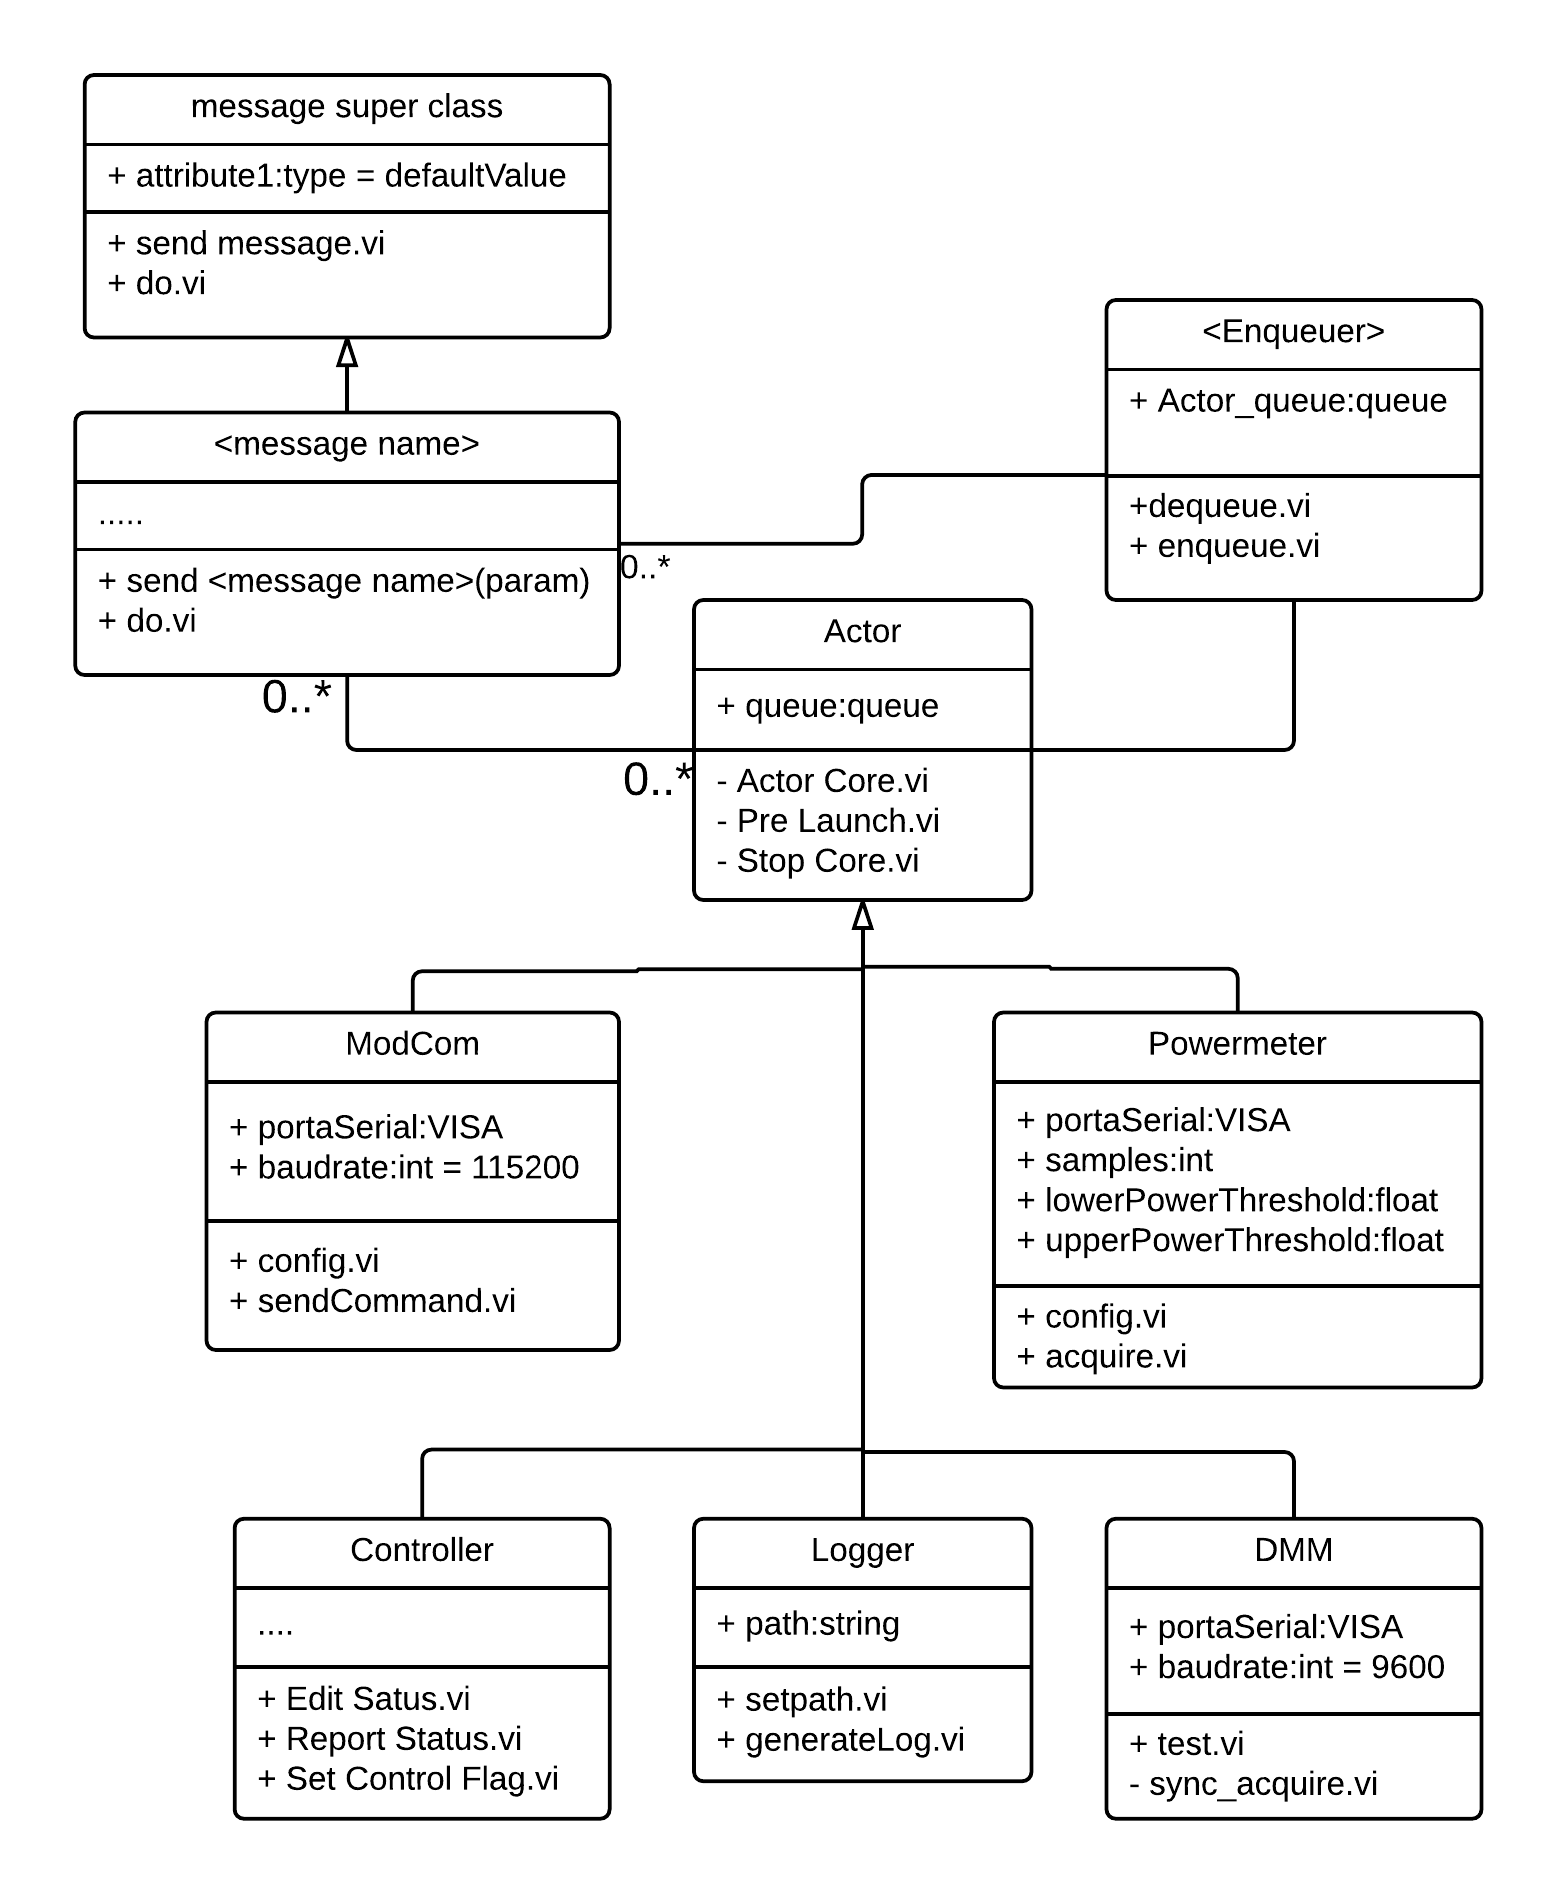
\includegraphics[width=1\linewidth]{model/class}
                \caption{Diagrama UML de classes simplificado retratando as classes do \textit{framework}, em conjunto com as classes de atores propostas e implementadas neste trabalho}
                \label{fig:classdiagram}
            \end{figure}
            
 
    \section{Implementação}
        
        Análoga à programação orientada a objetos, a implementação de um ator envolve a criação de métodos públicos e privados, sendo que todas as suas \textit{subVI} são privadas por padrão e podem ser acessíveis de maneira pública, se for criada uma classe de mensagem invocando-a. Dessa forma, o conjunto de classes de mensagens relacionadas àquele ator funciona como sua interface pública.
        
        Todas as implementações do módulos herdam da classes \texttt{actor} e \texttt{actor message} do \textit{framework} de atores. Todo ator tem que implementar a função \texttt{actor core.vi} para poder alterar o comportamento do ator. Como o próprio nome descreve, esta é a função núcleo do ator, responsável por sua inicialização e de seu tratador de mensagens. Também é possível e recomendável inserir nesta \texttt{vi} outras sub-rotinas, como, por exemplo, tratadores de eventos.    
        
        A interação dos atores filho com o \texttt{Controller} é realizada através de duas de suas classes de mensagens: \texttt{Set Control Flag}, que informa o status final de execução do teste e \texttt{Report Status}, que envia dados brutos do teste.
        
            
        \subsection{Ator de comunicação serial}
        \label{modcom}
        
            A comunicação serial em LabVIEW é realizada através de portas VISA (\textit{Virtual Instrument Software Architecture}) e são o padrão da National Instruments para configuração, programação, comunicação e depuração de sistemas de instrumentação. Dentro da VISA existe uma biblioteca própria para comunicação serial, que foi usada para criar as \textit{SubVI} base deste ator.
            
            O funcionamento deste ator é viabilizado pela \texttt{serialcore.vi}, a \textit{subVI} que envia comandos e captura respostas do dispositivo sob teste, como também confere respostas por padrões de \textit{strings}. É invocada diversas vezes por todos os outros métodos do ator. Esse funcionamento interno, assim como a relação do ator com agentes externos, estão ilustrados no diagrama da figura \ref{fig:diagserial}. 
            
            \begin{figure}
                \centering
                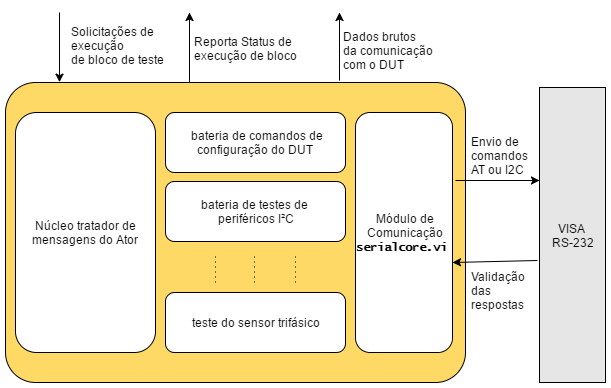
\includegraphics[width=1\linewidth]{fig/diag/blocoserial.png}
                \caption{Diagrama de blocos do \texttt{ModCOM}, ator de comunicação serial}
                \label{fig:diagserial}
            \end{figure}

            Todo o roteiro está escrito diretamente no código fonte do programa e as mensagens do \texttt{Controller} para o \texttt{ModCOM} consistem somente do pedido de execução de determinado bloco de teste interno. Devido à falta de generalização de sua interface,  este ator foi de longe aquele com o maior número de classes de mensagens. Para retornar dados brutos da comunicação com o módulo, o ator usa a mensagem \texttt{Report Status} do Controlador, que decide sobre a reexecução do bloco ou o término do teste.
            
            Por trabalhar com duas portas seriais, foram instanciados dois atores: para comunicar com o módulo por comandos AT e outro para acessar periféricos conectados no barramento  I$^{2}$C. 
            
            Apesar de não possuir uma interface gráfica de usuário própria, alguns métodos deste ator invocam as suas próprias. Destaca-se entre elas o teste de painel de LEDs, aonde foi empregado um painel esqueumórfico. Isso será mencionado na sessão \ref{ergo}, sobre ergonomia. 
        
            
            %De um ponto de vista externo o ator funciona da seguinte maneira:
            
            %Configura-se a porta através Após sua configuração - porta serial a ser usada, \textit{baudrate}, etc - o ator está pronto para comunicar com o módulo. Após receber do controlador o comando de testes para ser executado, o ator executa a rotina e reporta ao Controlador os dados de resposta, assim como o diagnóstico de aprovação ou reprovação.
            
            %Devido ao curto prazo dado ao projeto, nessa implementação inicial não foi implementado o interpretador para o padrão de roteiros utilizados no programa anterior. o que daria bastante flexibilidade à equipe para editar o roteiro conforme mudanças de \textit{firmware}, aplicação ou revisões de placa. Ao invés disso, todos os comandos são parte do código fonte do programa, situação conhecida como \textit{hardcoding}. No contexto desse projeto isto é considerado um antipadrão de projeto de software, já que assumimos que variável ambiental é constante. %todo cite anti patterns
            
        
        \subsection{Ator Multímetro}
            \label{dmmmodel}
            
            
            % falar da \texttt{sync_acquire vi} e como é a comunicação com ahrware e como é feita a Sincronização, tratamento do frame aquisiçaõ e envio de dados para a test.vi
            
            % falar da test.vi
            % como funciona o deboouncer e processo de validação de leitura do multimetro
            % GUI
            
            % que tipo de mensagens ele recebe do exterior.
            % configuração e acquisicao

            A implementação desta classe de ator, denominado \texttt{DMM}, começou pela função de aquisição e sincronia de \textit{frames}, acondicionados dentro da VI \texttt{sync\_acquire.vi}. Após a criação de uma interface de leitura serial do multímetro, foi criada uma máquina de estados para a sincronização dos \textit{frames}, já descritos pela figura \ref{fig:dmmprotocol}.
            
            
            Com a sincronização funcionando, desenvolveu-se um conjunto de SubVI para a conversão dos \textit{frames} em um \textit{cluster} com medidas e todas as informações adicionais que o multímetro fornece. Isso envolveu a decomposição dos \textit{frames}, conversão de código de sete segmentos em inteiros e associação de unidades de medida. 
            
            \texttt{test.vi} é a segunda VI fundamental deste ator, que checa as medidas recebidas de \texttt{sync\_acquire.vi} e provê uma interface gráfica de usuário para o operador de teste. A comunicação entre as duas VIs é feita através de uma fila. Sua interação dentro do ator é ilustrada pela figura \ref{fig:diagdmm}.
            
            \begin{figure}
                \centering
                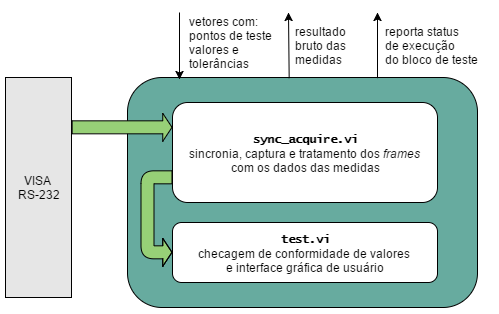
\includegraphics[width=0.9\linewidth]{fig/diag/diagdmm.png}
                \caption{Diagrama de blocos do \texttt{DMM}, ator de aquisição de medidas do multímetro digital}
                \label{fig:diagdmm}
            \end{figure}
            
            A checagem de medidas de \texttt{test.vi} é análoga a um algoritmo de \textit{debounce} de botão analógico e funciona em três estados:
            \begin{enumerate}
                \item Aguardar o valor da medida ficar dentro dos limites de tolerância para o valor de referência daquele ponto de medida. Exceção esperada: \textit{timeout}.
                \item Certificar-se de que a medida se mantém dentro da faixa de tolerância por um tempo especificado. Em caso de sucesso, ir para o estado 3 ou lançar uma exceção de erro de medida.
                \item Em caso de exceção, terminar o teste como reprovado ou permitir o reteste. Do contrário, passar para o próximo ponto de teste ou, se for o último ponto, aprovar a bateria de testes.
            \end{enumerate}

            Em caso do multímetro estar em um modo de operação incorreto, \texttt{test.vi} lança uma exceção e notifica o operador.  
            
            %colocar em erognomia?
            A interface gráfica de usuário (GUI) é exibida na figura \ref{fig:dmmfp}, onde o operador pode acompanhar as medições e qual ponto de teste deve deixar a ponta de prova. Também é notificado por sinais sonoros quando o ponto de teste é aprovado ou reprovado.
            
            \begin{figure}
                \centering
                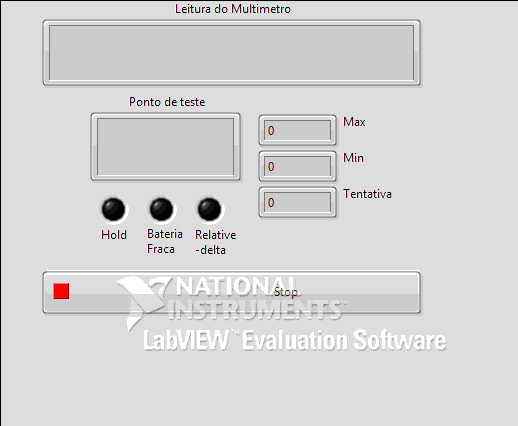
\includegraphics[width=0.8\linewidth]{lv/dmm/DMM_lvclass_DMM_UI_p}
                \caption{Painel da VI de aquisição de medidas do multímetro digital}
                \label{fig:dmmfp}
            \end{figure}
            
            Em termos de configuração, este ator precisa receber as seguintes informações: porta serial utilizada; tempo de estabilização de medida; número de tentativas; e o \textit{array} de pontos de teste com os seguintes atributos para cada ponto: \textit{limiar máximo; limiar mínimo; unidade de medida.}
            
            Assim como o ator \texttt{ModCOM}, o \texttt{DMM} utiliza-se do conjunto de mensagens do \texttt{Controller} para reportar o parecer final das medições, assim como os dados brutos de teste. 
            
            
        \subsection{Registrador de testes} 
            
            
            O gerenciador de registros, por sua baixa complexidade, foi implementado utilizando-se poucas VIs (figura \ref{fig:diaglog}). Este ator recebe do controlador de teste dois conjuntos de dados diferentes: os dados brutos da execução de teste e o cluster com os dados de teste resumidos. 
            A VI principal é \texttt{generateLog.vi}, que aglutina as conversões dos dados resumidos para JSON (\textit{JavaScript Object Notation}) e as dos dados brutos em documento de texto. 
            
              \begin{figure}
                \centering
                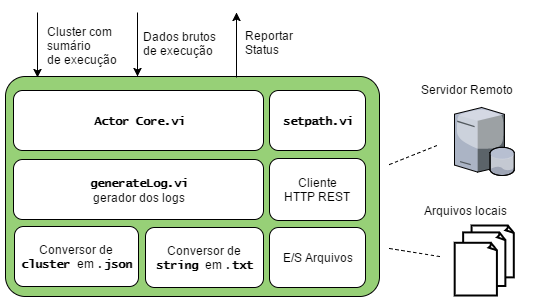
\includegraphics[width=0.9\linewidth]{fig/diag/diaglog.png}
                \caption{Diagrama de blocos do \texttt{logger}, ator atribuído de gerar arquivos de registro das baterias de testes}
                \label{fig:diaglog}
            \end{figure}
            
            
            % pertence à modelagem não?
            O registro com os dados brutos de execução contém o despejo da troca de mensagens pela serial, das medidas de tensão e potência, as exceções lançadas durante o teste e as métricas de desempenho. São dados necessários para a depuração e diagnóstico de problemas na placa e para melhor efetividade no retrabalho, sendo usados tanto em produção quanto em manutenção.
            
            A segunda classe de registro é um resumo estruturado da bateria de testes, o diagnóstico geral da placa e outras informações importantes para o controle e rastreamento dos produtos, requisito necessário para otimizações do processo produtivo, como também do próprio produto. Recebe o \textit{cluster} com os dados do DUT e resultados da bateria de teste e transforma em um objeto JSON.
            
            Quanto ao armazenamento, o ator suporta que seja feito tanto em servidor remoto, através de uma API REST, como também em pastas locais, através da biblioteca padrão de E/S de arquivos. O uso de arquivos locais é importante para o diagnóstico e depuração no local de fabricação, como também em situações sem conexão com a internet.
            
            
        \subsection{Sensoriamento de potência do \textit{front-end} RF}
        \label{pwmodel}
           
             
            % isso naõ é especificação?
            %Falar como a medida de potencia RF é realizada. Não é nenhum pouco conforme os padrões, mas serve para o propósito.
            
            %implementação
            O desenvolvimento deste ator foi simplificado com uso das bibliotecas e \textit{drivers} fornecidas pelo próprio fabricante. Estas bibliotecas possuem VIs de fácil utilização para configuração e aquisição de medidas e foram utilizadas na criação de \texttt{acquire.vi}, a VI principal deste ator. Esta VI recebe como entrada: frequência de medição, largura de banda, tamanho da janela de aquisição, número de amostras e limites máximo e mínimo de potência (em dBm). Seu funcionamento interno consiste em um laço simples de aquisição e comparação com a referência especificada. \texttt{config.vi} configura os dados internos do ator, como a porta USB utilizada. O ator pode ser visto na figura \ref{fig:diagpwmr}.
            
            \begin{figure}
                \centering
                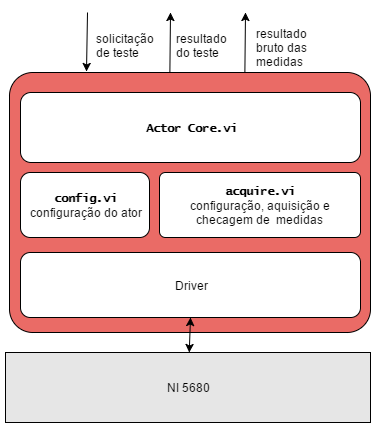
\includegraphics[width=0.7\linewidth]{fig/diag/diagpot.png}
                \caption{Diagrama de blocos do \texttt{PowerMeter}, ator de interface com o NI 5680}
                \label{fig:diagpwmr}
            \end{figure}
            
        \subsection{Controlador}
        
            % interface com outros atores - tipos de mensagem
            % funcionamento interno
            % como interage com o hardware
            % interface gráfica
            %extras    
            
            % Um geralzão dos módulos criados para fazer esse ator ser o que ele é. O que ele é? um ator de interface de usuário, watchdog e coordenador de atores filhos. 
            
            
            O \texttt{controller}, módulo de supervisão e controle de execução, é composto pelo módulo de inicialização de atores filhos e de dois laços acionados por eventos (figura \ref{fig:diagctrl}): a interface gráfica de usuário e o controle de fluxo de execução. 
            
            \begin{figure}
                \centering
                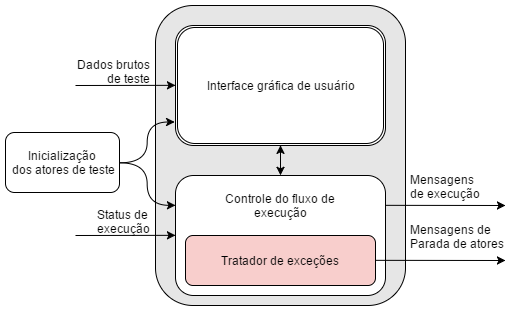
\includegraphics[width=0.9\linewidth]{fig/diag/diagctrl.png}
                \caption{Diagrama de blocos do \texttt{Controller}, ator supervisor}
                \label{fig:diagctrl}
            \end{figure}
            
            A escolha de uma estrutura orientada a eventos para o controle de fluxo de execução foi devido à sua sinergia com um sistema de atores e as trocas de mensagens entre eles. Dessa maneira, sempre que ele receber resposta de um ator filho, ele pode disparar outras mensagens de execução.
    
            O \texttt{Controller} possui o método \texttt{set control flag.vi} para que seus atores filhos relatem sucesso/falha de execução de subrotinas e baterias de testes. Para ser acessível às entidades externas ao ator, o método é exposto por uma classe de mensagem. Estas mensagens são usadas pelo bloco de controle de fluxo para alternar seu estado de execução e disparar outras mensagens para seus atores filhos.
            
            Outro método exposto por uma classe de mensagem é \texttt{report status.vi}, que é usada para transmitir ao \texttt{Controller} os registros de execução de teste e saída da porta serial. Todos os dados recebidos por estas mensagens vão para a interface de usuário, para depuração em tempo de execução e posteriormente, enviadas ao ator \texttt{Logger}.
            
            Seu tratador de exceção possui finalidades: parada, reinicialização e \textit{watchdog} de atores filhos e, como próprio sugere, tratamento de falhas de execução. Parte dele foi implementado a partir das funções de tratamento de erro do LabVIEW, do \textit{Actor Framework} e outras funções customizadas, especialmente para casos de desconfiguração de instrumentos de medida.
            
            A figura \ref{fig:cntrlpanel} expõe a interface de usuário do programa, que oferece ao usuário duas saídas de texto: despejo da comunicação serial, à esquerda, e o registro de execução das baterias de teste e medições, à direita. 
            
            \begin{figure}
                    \centering
                    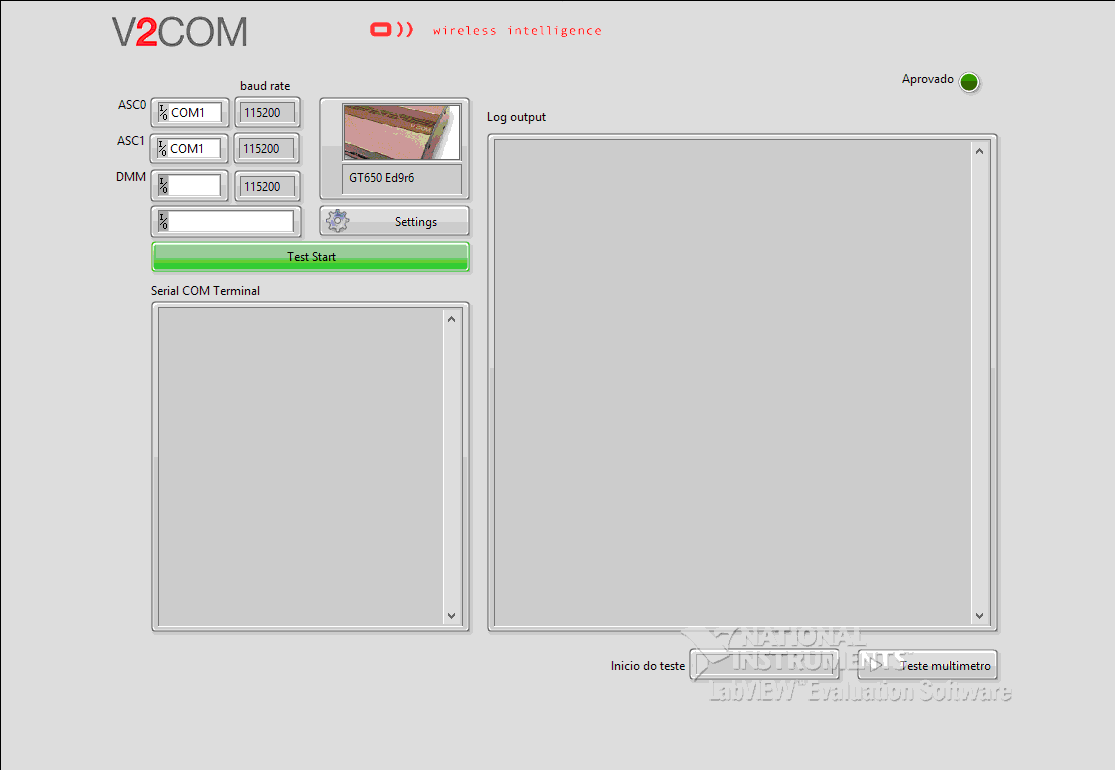
\includegraphics[width=0.8\linewidth]{lv/controler/Controller_lvclass_Actor_Corep}
                    \caption{Tela do painel principal de interface de usuário}
                    \label{fig:cntrlpanel}
            \end{figure}
        
        \subsection{Ergonomia}
        \label{ergo}
            
            % leds simulacro (sem uso do teclado
            % multimetro e a reduçaõ do uso do teclado
            % duas telas de depuracao
            
            A ergonomia no trabalho envolvido foi considerada durante todo o projeto e desenvolvimento do programa. As etapas de teste que envolvem a interação do trabalhador foram pensadas de forma a minimizar o esforço repetitivo e o desgaste do operador. No que confere à parte de software, o interesse é minimizar o uso do teclado e mouse, bem como a necessidade de dividir atenção visual entre o DUT e o monitor. As partes principais onde o operador precisa interagir com o software são: teste dos LEDs do painel, medição de tensões com o multímetro e testes de alimentação e bateria. 
            
            Para o teste do painel de LEDs do DUT foi criada uma GUI esqueumórfica (figura \ref{fig:modcomledp}) para facilitar a comparação com o painel real, agilizando e diminuindo erros no processo de verificação visual.
            
            \begin{figure}
                \centering
                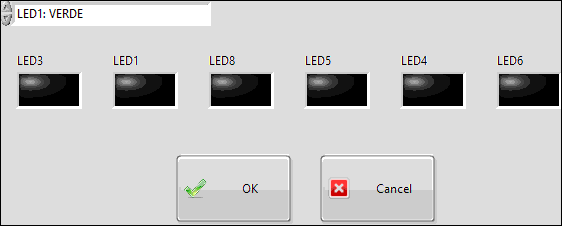
\includegraphics[width=0.8\linewidth]{lv/modcom/ModCOM_LED_popupp.png}
                \caption{Captura de tela do Painel de teste de led}
                \label{fig:modcomledp}
            \end{figure}
            
            Quanto às medições de tensões na placa, as mãos e atenção do operador se voltam para a DUT. Descuidos aqui podem causar erros ou, até mesmo, danos ao circuito. Em relação a isto, foi criado um \textit{debouncer} para validação das medidas, permitindo que o operador passe a ponteira pelos pontos de medição sem a necessidade de digitar ou interagir com o teclado. Além disso, referências sonoras foram criadas para os casos de aprovação, repetição ou reprovação de medição, de forma que a atenção visual do operador não precise desviar do DUT para o computador.
            
            Dentre as outras melhorias citam-se: a separação de uma tela dedicada somente ao registro da comunicação com o módulo para a melhor depuração; a redução de etapas de digitação por teclas simples ou mouse. 
        
\clearpage

    \chapter{Resultados e Análise}
\label{result}    
    
\section{Resultados e Análise de Desempenho}
    
    Com o programa pronto para ser validado, foi montado um esquema de teste para avaliação interna de desempenho do programa de testes, antes de entrar em produção na fábrica. A intenção era de compará-lo em relação à versão em Java e também detectar erros de software que possam ter passado despercebidos durante o desenvolvimento. Foram separadas cerca de 5 placas do GT650 para teste. Cada uma delas foi testada duas vezes por cada um dos dois programas, totalizando 20 execuções. O teste foi executado pelo autor em bancada de desenvolvimento.
        
    A tabela \ref{tab:resultado} exibe as médias do tempo de execução de teste para os dois programas. Nota-se, pela tabela, uma redução de quase 7 segundos no tempo médio de teste do programa reescrito em relação ao programa legado. É possível observar que estes resultados são atribuídos somente pelas mudanças ergonômicas do programa, já que o roteiro é idêntico ao anterior. Questões de velocidade de processamento entre as linguagens não refletiram em muitas mudanças, se for considerado que nenhuma das atividades exige uso intenso de CPU, já que consiste de rotinas de comunicação e tratamento de dados em baixa velocidade. O gargalo do teste é a própria velocidade de resposta do dispositivo sob teste e das interações com o operador, como nos testes com o multímetro. Certamente que resultados melhores podem ser obtidos se aproveitados os recursos de concorrência de software que \textit{framework} oferece, mas infelizmente não foi possível tratar os despejos de teste e comparar as diferenças de execução, bloco a bloco, do roteiro de teste.
        
    \begin{table}[h]
        \centering
        \caption{Média e desvio padrão das 20 amostras de teste de bancada}
        \label{tab:resultado}
        \begin{tabular}{l|cc}
        
                          & Programa Legado & Programa Reescrito \\
    \hline
            Média (s)         & $33.65\pm2.43$          & $26.24\pm3.37$                          \\
        \end{tabular}
    \end{table}
    
    Nota-se também que a distribuição dos tempos de teste do programa novo é ligeiramente mais difusa do que o do programa antigo, o que pode ser atribuído à falta de hábito na operação do software.

\section{Análise da implementação}

    A falta de um analisador de linguagem de marcação que interprete os roteiros de teste dificulta que este programa entre em operação em fábrica pois, no esquema atual, qualquer alteração no roteiro de teste requer uma nova compilação do programa.
    
    Além da questão de flexibilidade do roteiro de teste, ainda é necessário que o programa passe por uma etapa maior de testes controlados e exposição a erros de produção controlados, a fim de depurar erros de programa como também melhorar os tratadores de exceção.
   
    O ambiente LabVIEW permite ter uma visão clara do fluxo de sinais e seu \textit{multithreading} natural permite a realização de sistemas concorrentes com facilidade. Entretanto, a implementação do modelo de atores ficou comprometida pelas limitações do seu \textit{framework} em LabVIEW, principalmente pela impossibilidade de livre comunicação entre atores sem relação pai-filho, e também porque a criação de classes de mensagens depende de macros para serem geradas, o que enrijeceu o processo de desenvolvimento. O uso da linguagem gráfica do ambiente LabVIEW, apesar de simples para pequenas rotinas, torna-se complicado e difícil de refatorar, se aplicado a programas maiores, e sua implementação do paradigma orientado a objetos, assim como do modelo de atores, é demasiadamente complicada e problemática de usar.
    Uma maneira de contornar isto seria talvez a utilização do Labwindows/CVI, o ambiente C da National Instruments, ou o uso do LabVIEW somente em partes aonde ele se sobressalta como melhor opção. Isso permitiria melhor controle de versão, refatoração de código, revisão por pares e aplicação de boas práticas de programação textual. 
    
   
\chapter{Conclusão}
\label{conclusao}

    Neste trabalho foi possível mostrar a aplicação do \textit{framework} de atores para a solução de problemas de final de linha de montagem de placas eletrônicas. O trabalho conseguiu cumprir com os requisitos de modularidade e flexilidade de implementação, porém foi limitado pela falta de um interpretador de arquivos de configuração que estendesse a flexibilidade do sistema à equipe de teste no local de produção. No que diz respeito à produtividade, uma atualização de jiga de teste pode melhorar a taxa de produção, e no caso particular das jigas com chaveamento de instrumentos de teste, o sistema de atores e o uso de concorrência pode ser melhor explorado.
    
    \section{Trabalhos futuros}          
    Dentre as melhorias interessantes para o processos de teste de placas eletrônicas, destacam-se:
    \begin{itemize}
            
        \item Um interpretador de roteiro para flexibilização da execução de testes e para poder testar outros produtos com as mesmas ferramentas de software;
        
        \item Um escalonador e gerenciador de recursos para o uso com uma jiga multiplexada para teste de múltiplas unidades simultâneas;
        
        \item  Criar uma linguagem de marcação para os roteiros de teste que dê suporte ao sistema de atores e otimize o tempo de execução;

        \item Construção de uma jiga de testes que suporte múltiplas placas de circuito impresso testadas simultaneamente. No aspecto de software, isso demandaria a reescrita do controlador ou o desenvolvimento de um ator de hierarquia superior.
    \end{itemize}
    
    É possível melhorar consideravelmente a qualidade do teste ao aplicar técnicas de \textit{projeto orientado à testabilidade} em uma nova revisão do produto. Essa opção, apesar de custosa à equipe de projeto, possui um bom retorno de investimento. Outra possibilidade de melhoria seria a partir de uma análise de cobertura de faltas, transformando isto em uma nova especificação de baterias de teste. 
    
    Ambas as propostas só se tornam viáveis conforme a relevância do volume de perdas durante a produção e dos retornos para manutenção, especialmente aqueles que se enquadram nos casos de \textit{causa desconhecida} no controle de qualidade.
        
    \section{Palavras finais}
    
    Feitas as críticas, ressalta-se que o modelo de atores possui potencial para a implementação de rotinas de teste concorrente e escalona bem para aplicações maiores. O arranjo de módulos desacoplados foram implementados com sucesso e sua interação em teste desempenhou conforme esperado. Os avanços na ergonomia da interface mostraram-se também relevantes à produtividade e nas melhorias de condição de trabalho.
    
    O trabalho foi proveitoso no aprendizado de técnicas de teste e diagnóstico de sistemas eletrônicos e suas aplicações durante os processos de manufatura, operação e manutenção. Constatou-se também que o uso de técnicas e boas práticas de desenvolvimento de software facilitam a manutenção e melhorias ao longo dos anos, prevenindo retrabalho e otimizando o tempo de desenvolvimento.
    

% ----------------------------------------------------------
% ELEMENTOS PÓS-TEXTUAIS
% ----------------------------------------------------------
\postextual
% ----------------------------------------------------------

%\bibliographystyle{plain}
\bibliographystyle{apalike}

\bibliography{references}
\end{document}

% --- 
% https://github.com/mateusduboli/ufsc-thesis-latex
% ---------------------------------------------------------
